\documentclass[11pt, a4paper]{article}

% AA Lingua E Codifica
\usepackage[italian]{babel}
\usepackage[utf8]{inputenc}
\usepackage[T1]{fontenc}
\usepackage{lmodern}

% AA Layout Di Pagina E Tipografia
\usepackage[margin=2cm, top=1.5cm, bottom=1.5cm]{geometry}
\usepackage{parskip}
 \usepackage[expansion=false]{microtype}

% AA Gestione Dei Colori
\usepackage[table]{xcolor}
\definecolor{primary}{RGB}{30, 90, 160}
\definecolor{accent}{RGB}{20, 60, 120}
\definecolor{subtext}{RGB}{90, 95, 100}
\definecolor{transducerRed}{RGB}{195, 60, 55}
\definecolor{greenLine}{RGB}{35, 145, 65}
\definecolor{refline}{RGB}{50, 110, 190}
\definecolor{pointFill}{RGB}{250, 185, 45}
\definecolor{pointDraw}{RGB}{210, 130, 20}
\definecolor{good}{RGB}{35, 145, 65}
\definecolor{bad}{RGB}{205, 50, 45}

\definecolor{govBg}{RGB}{244, 248, 244}
\definecolor{robBg}{RGB}{242, 246, 252}
\definecolor{envBg}{RGB}{254, 244, 244}
\definecolor{cmdBlue}{RGB}{30, 80, 160}
\definecolor{actRed}{RGB}{190, 30, 30}
\definecolor{measGreen}{RGB}{20, 140, 60}
\definecolor{unitFill}{RGB}{232, 238, 248}

\definecolor{poleN}{RGB}{200, 45, 40}
\definecolor{poleS}{RGB}{25, 85, 155}
\definecolor{rotorFill}{RGB}{246, 248, 252}
\definecolor{forceColor}{RGB}{195, 30, 30}
\definecolor{bField}{RGB}{140, 160, 185}

% AA Matematica E Simboli
\usepackage{amsmath, amssymb, amsfonts}
\usepackage{mathtools}
\usepackage{siunitx}
\DeclareSIUnit\rpm{rpm}

% AA BB OTTIMIZZAZIONE MATRICI LUNGHE PER LA STAMPA
\setlength{\arraycolsep}{10pt}
\usepackage{bm}

% AA Grafica, Immagini E Tabelle
\usepackage{graphicx}
\graphicspath{{./Images/Lab}}
\usepackage{float}

% --- RIDUZIONE SPAZI FIGURE E CAPTION ---
% Spazio Sopra E Sotto Le Figure [H] (default: 12pt)
\setlength{\intextsep}{6pt plus 1pt minus 1pt}
% Spazio Per Figure In Alto/Basso [t]/[b] (Default: 20pt)
\setlength{\textfloatsep}{8pt plus 1pt minus 1pt}
% Spazio Tra L'immagine E La Caption (Default: 10pt)
\setlength{\abovecaptionskip}{6pt}
% Compensa Lo Spazio Extra Aggiunto Da \usepackage{parskip}
\setlength{\belowcaptionskip}{-4pt}
% ----------------------------------------

\usepackage{booktabs}
\usepackage{array}
\usepackage{multirow}
\usepackage{tabularx}
\usepackage{listings}
\usepackage{tikz}
\usetikzlibrary{shapes.geometric, arrows.meta, positioning, fit, calc, quotes}

% AA Link, Riferimenti Ed Elenchi
\usepackage[unicode]{hyperref}
\hypersetup{
    colorlinks=true,
    linkcolor=blue,
    urlcolor=blue,
    citecolor=blue,
    pdftitle={Titolo Del Documento},
    pdfauthor={Francesco Lo Verde},
    pdfpagemode=FullScreen,
}
\usepackage{bookmark}
\usepackage[italian,capitalize]{cleveref}
\usepackage{enumitem}
\setlist{noitemsep}

% AA Personalizzazione Titoli E Altri Pacchetti
\usepackage{titlesec}
\titleformat{\section}{\normalfont\LARGE\bfseries}{\thesection}{0.75em}{}
\titleformat{\subsection}{\normalfont\Large\bfseries}{\thesubsection}{0.75em}{}
\titleformat{\subsubsection}{\normalfont\large\bfseries}{\thesubsubsection}{0.75em}{}
\titlespacing*{\section}{0pt}{1.2ex plus 0.4ex minus 0.1ex}{0.8ex plus 0.01ex}
\titlespacing*{\subsection}{0pt}{1.0ex plus 0.3ex minus 0.1ex}{0.6ex plus 0.01ex}
\titlespacing*{\subsubsection}{0pt}{0.8ex plus 0.2ex minus 0.1ex}{0.4ex plus 0.05ex}

\usepackage{comment}
\newtheorem{theorem}{Definizione}


\author{Francesco Lo Verde}

\begin{document}

\tableofcontents

\newpage
% AA Parte 1 - Sistemi Di Misura E Sensori Per La Robotica
\section{Introduzione Alla Percezione Nei Sistemi Robotici}
Negli organismi viventi, la percezione dipende da organi sensoriali come occhi o orecchie, mentre gli stimoli fisici vengono convertiti in impulsi elettrici tramite il sistema nervoso.\\
In robotica, questa struttura viene replicata tramite i \textbf{sensori}, che permettono al robot di interagire con l'ambiente e correggere eventuali errori di posizione o orientamento e i \textbf{traduttori} che convertono grandezze fisiche in segnali elettrici. I sensori e i trasduttori sono fondamentali per il controllo in anello chiuso, poiché forniscono informazioni sullo stato del sistema e sull'ambiente circostante.

I dispositivi di misura impiegati nei sistemi robotici quantificano grandezze fisiche analoghe a quelle biologiche:
\begin{itemize}
    \item \textbf{Visione}: telecamere ottiche, stereoscopiche e sensori di profondità (LIDAR, camere RGB-D);
    \item \textbf{Tatto}: encoder ottici d'asse e sensori di coppia ai giunti;
    \item \textbf{Percezione Acustica} : trasduttori piezoelettrici (sonar) e microfoni per il monitoraggio predittivo;
    \item \textbf{Parametri Ambientali} (temperatura degli avvolgimenti, gradienti termici): dispositivi a variazione di resistenza o a potenziale termoelettrico.
\end{itemize}

\section{Dispositivi Di Misura E Definizioni Fondamentali}

\subsection{Esempio Pratico: La Misura Della Temperatura}

La \textbf{temperatura} è grandezza scalare che indica l'energia cinetica media del moto delle particelle. Esistono molti strumenti che permettono di stimare la temperatura di un corpo (\textit{misurando}) attraverso differenti principi fisici:
\begin{figure}[H]
    \centering
    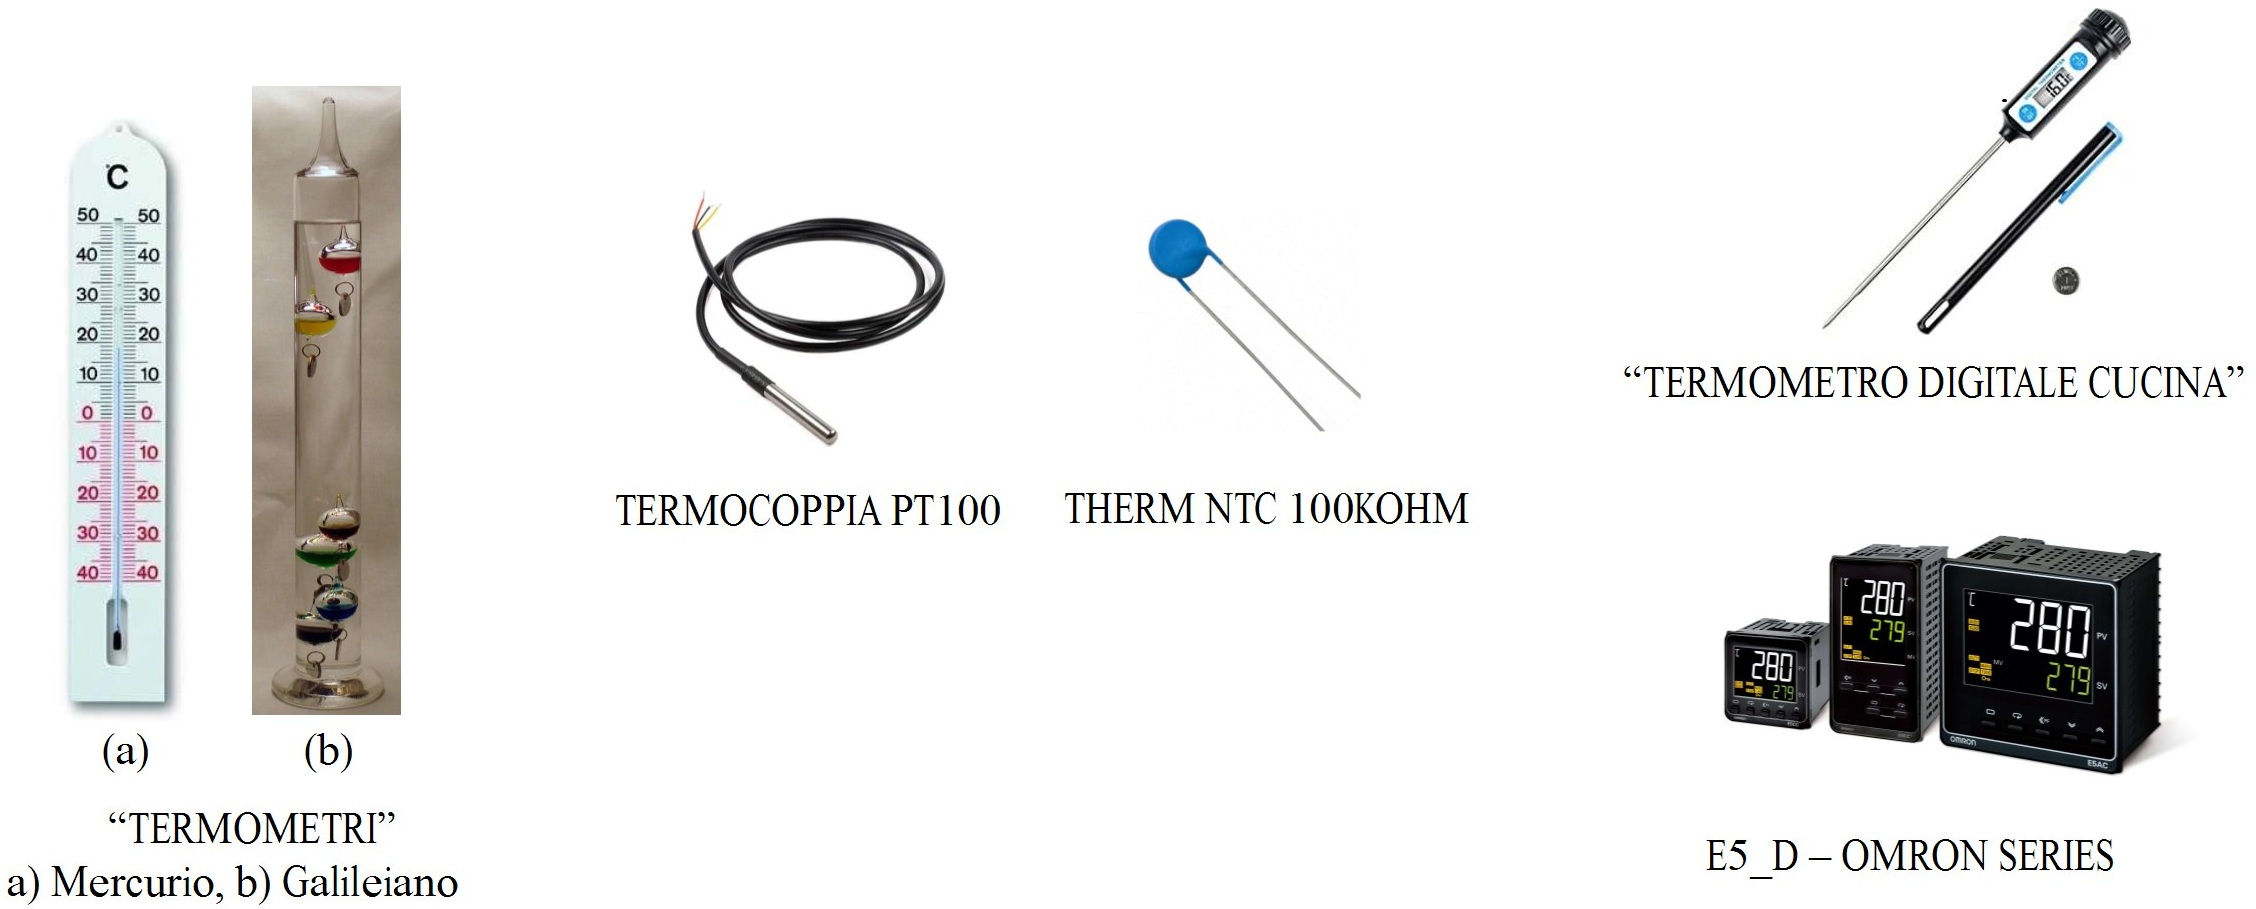
\includegraphics[width=0.8\textwidth]{Images/Lab/DispTemp.jpg}
    \label{fig:termometri}
\end{figure}
\begin{itemize}
    \item[(a)] Il \textbf{Termometro A Mercurio} sfrutta il coefficiente di dilatazione del liquido dentro un capillare di vetro
    \item[(b)] Il \textbf{Termometro Di Galileo} sfrutta la variazione di densità di un fluido idrocarburico con la temperatura, inducendo galleggiamento o affondamento per spinta di Archimede di ampolle tarate
    \item[(c)] La \textbf{Termoresistenza PT100} (RTD \textit{Resistance Temperature Detector}) che permette di misurare la temperatura in base alla variazione della resistività del platino ($R_0 = \SI{100}{\ohm}$ a $\SI{0}{\celsius}$);
    \item[(d)] Il \textbf{Termistore NTC} (\textit{Negative Temperature Coefficient}) è un semiconduttore ceramico la cui resistenza decresce in modo non lineare con la temperatura;
    \item[(e)] Il \textbf{Termometro Digitale Da Cucina} e il \textbf{Termoregolatore Industriale} (es. serie OMRON E5\_D) sono sistemi integrati provvisti di alimentazione, stadi di condizionamento, convertitore analogico-digitale, microcontrollore e interfaccia utente.
\end{itemize}

\newpage
Si possono dividere questi dispositivi in tre classi principali
\begin{itemize}
    \item \textbf{Dispositivi Tradizionali Meccanico-Fluido-Dinamici} come i termometri a dilatazione e galileiani:
    \begin{itemize}
        \item \textbf{Stima Diretta:} forniscono lettura visiva immediata tramite lo spostamento di un indice graduato solidale al fluido o alla galleggiabilità di un corpo immerso.
        \item \textbf{Autonomia Energetica:} non richiedono alimentazione esterna e l'energia per lo spostamento meccanico è ricavata dalla differenza termica tra ambiente e sensore.
        \item \textbf{Scala Di Riferimento Incorporata:} la conversione è garantita geometricamente da una scala graduata solidale (es. in $\si{\celsius}$ o $\si{\kelvin}$).
    \end{itemize}
    \item \textbf{Sensori Discreti A Uscita Elettrica} come la PT100 o le Termocoppie:
    \begin{itemize}
        \item \textbf{Uscita Non Direttamente Fruibile:} il componente non fornisce una lettura visiva diretta dello stato termico.
        \item \textbf{Necessità Di Circuiti Ausiliari:} richiedono polarizzazione esterna (es. ponti di Wheatstone per PT100 o partitori di tensione) e convertitori analogico-digitali (ADC).
        \item \textbf{Natura Elettrica Del Segnale:} la variazione termica è convertita in modulazione di impedenza ($\Delta R(T)$) o tensione ($\Delta V(T)$), compatibile con microcontrollori e PLC.
    \end{itemize}
    \item \textbf{Strumenti E Sistemi Di Controllo Integrati} come termometri digitali e termoregolatori:
    \begin{itemize}
        \item \textbf{Stima Diretta Ed Elaborata:} visualizzano il valore numerico su display nell'unità di misura selezionata.
        \item \textbf{Architettura A Più Livelli:} integrano l'elemento primario con elaborazioni di linearizzazione matematica e filtraggio digitale.
    \end{itemize}
\end{itemize}

\subsection{Definizione Formale Di Sistema Di Misura}
Un sistema di misura può essere schematizzato come una \textit{Black Box} che riceve in ingresso il \textbf{misurando} $x(t)$ e produce in uscita una stima $y(t)$ del suo valore. Nei sistemi per la robotica, questa architettura può essere rappresentata una catena di acquisizione composta da tre stadi funzionali:

\begin{center}
    \begin{tikzpicture}[
        scale=0.75,
        transform shape,
        font=\sffamily,
        >=Stealth,
        line width=1.2pt,
        % Stile ellisse iniziale (Ambiente)
        ambiente/.style={
            ellipse,
            fill=primary,
            text=white,
            font=\sffamily\bfseries,
            align=center,
            inner sep=0pt,
            minimum width=3.2cm,
            minimum height=1.6cm
        },
        % Stile blocchi della catena
        blocco/.style={
            rectangle,
            rounded corners=4pt,
            fill=primary,
            text=white,
            font=\sffamily\bfseries\small,
            align=center,
            inner sep=8pt,
            minimum width=2.8cm,
            minimum height=1.6cm
        },
        % Stile etichette sulle frecce (Ingresso / Uscita)
        label-sopra/.style={
            font=\sffamily\bfseries\small,
            text=black,
            above=3pt,
            align=center
        },
        label-sotto/.style={
            font=\sffamily\footnotesize,
            text=subtext,
            below=3pt,
            align=center
        },
        % Frecce di collegamento
        flusso/.style={
            ->,
            draw=accent,
            line width=1.5pt
        }
    ]

        % 1. Ambiente (sorgente esterna)
        \node[ambiente] (env) {Ambiente};

        % 2. Blocchi della catena di misura
        \node[blocco, right=2.8cm of env] (sense) {Sensore/Trasduttore};
        \node[blocco, right=1.0cm of sense] (cond) {Condizionamento \\Del Segnale};
        \node[blocco, right=1.0cm of cond] (proc) {Elaborazione \\Del Segnale};

        % 3. Frecce interne tra i blocchi
        \draw[flusso] (sense) -- (cond);
        \draw[flusso] (cond) -- (proc);

        % 4. Freccia di Ingresso con testo sopra e sotto (spostato a sinistra)
        \draw[flusso] (env.east) -- (sense.west)
            node[midway, label-sopra, xshift=-0.35cm] {Ingresso}
            node[midway, label-sotto, xshift=-0.35cm] {(Grandezza \\Da Misurare)};

        % 5. Freccia di Uscita con testo sopra e sotto (spostato a destra)
        \draw[flusso] (proc.east) -- ++(3.2cm, 0)
            node[midway, label-sopra, xshift=0.35cm] {Uscita}
            node[midway, label-sotto, xshift=0.35cm] {(Valore Misurato)};

        % 6. Grande riquadro esterno (Sistema di misura)
        \node[draw=accent, line width=1.8pt, rounded corners=6pt,
            inner ysep=14pt, inner xsep=12pt,
            fit={(sense) (proc)}] (sistema) {};

    \end{tikzpicture}
\end{center}

L'architettura funzionale è costituita da tre stadi sequenziali:

\begin{enumerate}
    \item \textbf{Sensore/Trasduttore (\textit{Sensing Element}):}
    È l'elemento che interagisce con la grandezza fisica da misurare e, in risposta alle sue variazioni, genera un segnale in uscita correlato al misurando che può essere di meccanico, elettrico oppure otticao, a seconda della tipologia di sensore utilizzato.

    \item \textbf{Condizionamento Del Segnale (\textit{Signal Conditioner}):}
    Si occupa di adattare il segnale proveniente dal sensore alle caratteristiche richieste dagli stadi successivi. In particolare, può amplificare segnali di basso livello, come quelli dell'ordine dei microvolt ($\si{\micro\volt}$) o dei millivolt ($\si{\milli\volt}$), portarli in intervalli standard, come $0$--$\SI{10}{\volt}$ o $\SI{4}{\milli\ampere}$--$\SI{20}{\milli\ampere}$, filtrare il rumore e correggere eventuali non linearità del sensore.

    \item \textbf{Elaborazione Del Segnale (\textit{Signal Processing}):}
    Si occupa dell'acquisizione e dell'elaborazione del segnale, effettuando, quando necessario, la conversione analogico-digitale (ADC). Il dato può quindi essere elaborato ulteriormente, e convertito nell'unità di misura desiderata, per poi essere inviato a un sistema esterno (come un controller o una FPGA)
\end{enumerate}

\newpage

\subsection{Distinzione Tra Concettuale Sensore E Trasduttore}

In robotica, \textit{sensore}, \textit{trasduttore} e \textit{attuatore} assumono delle definizioni rigorose

\begin{description}
    \item[Sensore:] dispositivo che \textbf{rileva} una grandezza fisica e genera un segnale informativo correlato, interpretabile da un sistema di acquisizione e elaborazione. La sua funzione principale è \textit{acquisire l'informazione}.
    \item[Trasduttore:] dispositivo che \textbf{converte} una forma di energia in un'altra. La sua funzione principale riguarda la conversione, non necessariamente finalizzata alla misurazione
\end{description}

In robotica si impiegano principalmente \textbf{trasduttori elettrici}, progettati per convertire forme di energia non elettrica (meccanica, termica, ottica, magnetica) in energia elettrica (tensione, corrente, carica), come mostrato in figura:

\begin{center}
    \begin{tikzpicture}[
        scale=0.85,
        transform shape,
        font=\sffamily,
        >=Stealth,
        line width=1.2pt,
        % Blocco centrale
        blocco/.style={
            rectangle,
            rounded corners=5pt,
            fill=transducerRed,
            text=white,
            font=\sffamily\bfseries,
            align=center,
            inner sep=10pt,
            minimum width=3.4cm,
            minimum height=3.0cm
        },
        % Testo sopra le frecce
        label-sopra/.style={
            font=\sffamily\bfseries\small,
            text=black,
            above=3pt,
            align=center
        },
        % Testo sotto le frecce (esempi o note)
        label-sotto/.style={
            font=\sffamily\footnotesize,
            text=subtext,
            below=3pt,
            align=center
        },
        % Frecce di flusso
        flusso/.style={
            ->,
            draw=accent,
            line width=1.5pt
        }
    ]

        % 1. Linea orizzontale tratteggiata verde (disegnata prima, così passa "dietro" al blocco)
        \draw[draw=greenLine, dashed, line width=1.6pt, dash pattern=on 8pt off 6pt]
            (-6.2, 0) -- (6.2, 0);

        % 2. Blocco centrale "Trasduttore"
        \node[blocco] (trans) {TRASDUTTORE};

        % Freccia in ingresso da sinistra
        \draw[flusso] (-5.8, 0.85) -- ([yshift=0.85cm]trans.west)
            node[midway, label-sopra] {Forma di Energia A};

        % Freccia in uscita a destra
        \draw[flusso] ([yshift=0.85cm]trans.east) -- (5.8, 0.85)
            node[midway, label-sopra] {Forma di Energia B}
            node[midway, label-sotto] {(es. Segnale Elettrico)};

        % Freccia da destra verso il blocco
        \draw[flusso] (5.8, -0.85) -- ([yshift=-0.85cm]trans.east)
            node[midway, label-sopra] {Forma di Energia B}
            node[midway, label-sotto] {(es. Segnale Elettrico)};

        % Freccia dal blocco verso sinistra
        \draw[flusso] ([yshift=-0.85cm]trans.west) -- (-5.8, -0.85)
            node[midway, label-sopra] {Forma di Energia A};

    \end{tikzpicture}
\end{center}

Grazie alla \textbf{Reversibilità Energetica}, la conversione può realizzarsi in verso opposto, ovvero trasformare grandezze elettriche in grandezze meccaniche, termiche o acustiche. Un trasduttore configurato in questo modo per produrre forze o coppie è detto \textbf{attuatore}. In un manipolatore, un servomotore sincrono a magneti permanenti (\textit{brushless} DC) è un trasduttore elettromeccanico che converte la potenza elettrica fornita dall'inverter in potenza meccanica rotazionale ($\tau \cdot \omega$) all'albero del giunto.

\subsection{Il Confine Tra Sensore E Trasduttore Nella Pratica}

La classificazione tra sensore e trasduttore dipende dalla scala di osservazione:
\begin{enumerate}
    \item \textbf{Sensori Che Incorporano Trasduttori:} nel manometro a tubo, la pressione del fluido agisce su un condotto metallico curvo a forma di C, chiuso a un'estremità. Quando la pressione aumenta, il tubo tende a deformarsi, provocando lo spostamento della sua estremità chiusa. Questo movimento meccanico viene trasmesso, attraverso un apposito meccanismo, a un ago che ruota su una scala graduata, permettendo così di visualizzare il valore della pressione. In questo modo, il manometro converte una grandezza fisica, la pressione, in uno spostamento meccanico facilmente leggibile.

    \item \textbf{Sensori Modulatori Privi Di Conversione Diretta:} nella fotoresistenza (LDR, \textit{Light Dependent Resistor}), che modifica la propria resistenza in base alla luce modifica ma non genera direttamente energia elettrica, quindi è necessario utilizzare una sorgente di alimentazione esterna per misurare la variazione di resistenza.

    \item \textbf{Trasduttori Costituiti Da Catene Di Sensori:} una cella di carico permette di misurare una forza trasformandola in una tensione elettrica. Quando viene applicata una forza, il corpo elastico al suo interno si deforma e questa deformazione viene rilevata attraverso la variazione di una resistenza elettrica. Poi attraverso uno specifico circuito, questa variazione viene convertita in una tensione proporzionale alla forza applicata.
\end{enumerate}
\newpage

\section{Caratteristiche Dei Sensori}

Le caratteristiche dei sensori si dividono in:

\begin{itemize}
    \item \textbf{Caratteristiche Statiche:} Descrivono la risposta del sensore a regime stazionario, ossia quando il misurando è costante o varia con dinamiche sufficientemente lente da rendere trascurabili i fenomeni transitori.
    \item \textbf{Caratteristiche Dinamiche:} Descrivono la risposta del sensore quando il misurando varia nel tempo e quindi non è possibile trascurare gli effetti transitori
\end{itemize}

\subsection{Caratteristiche Statiche}
\begin{itemize}
    \item \textbf{Accuratezza} (\textit{Accuracy}): Indica la vicinanza (\textit{closeness of agreement}) tra la media delle misure e il \textbf{valore vero} del misurando. In pratica, un elevata accuratezza è sinonimo di assenza di errori sistematici (offset o derive non compensate).
    \item \textbf{Precisione} (\textit{Precision}): Indica la vicinanza tra misure indipendenti ottenute applicando ripetutamente lo stesso procedimento sullo stesso misurando. Descrive l'ampiezza della \textbf{dispersione statistica} indotta da errori casuali.
    \item \textbf{Risoluzione} (\textit{Resolution}): Indica la più piccola variazione dell'ingresso $\Delta x_{min}$ che produce un'uscita osservabile. Per un encoder assoluto a 12 bit su un giro completo si ha:
    \[
        \Delta \theta_{\min} = \frac{2\pi}{2^{12}} = \frac{2\pi}{4096} \approx \SI{1.53e-3}{\radian} \approx 0.088^{\circ}
    \]
    \item \textbf{Sensitività} (\textit{Sensitivity}): Indica di quanto varia l'uscita al variare dell'ingresso ed è rappresentata dal rapporto tra l'uscita $\Delta y$ e l'ingresso $\Delta x$. La sensitività locale $S(x)$, data la caratteristica del sensore $f(x)$, è data dal limite dalla derivata prima della caratteristica del sensore
    \[
        S(x) = \frac{f(x)}{dx}
    \]
    Nel caso di un sensore con caratteristica lineare ($f(x) = Kx + c$) la sensitività è costante e pari alla pendenza $K$ della caratteristica. Nei sensori non lineari (sensori reali) varia in funzione dell'ingresso fino alla regione di \textbf{\underline{saturazione}}, ovvero quando piccole variazioni dell'ingresso non producono variazioni dell'uscita, ovvero si annulla la sensibilità per determinate variazioni dell'ingresso
\end{itemize}

\begin{center}
    \begin{tikzpicture}[
        scale=0.9,
        transform shape,
        font=\sffamily,
        >=Stealth,
        % Stile ellisse "Ambiente"
        ambiente/.style={
            ellipse,
            fill=primary,
            text=white,
            font=\sffamily\bfseries,
            align=center,
            inner sep=4pt,
            minimum width=3.0cm,
            minimum height=1.7cm
        },
        % Stile box del sensore
        sensorbox/.style={
            rectangle,
            rounded corners=5pt,
            fill=white,
            draw=accent,
            line width=1.4pt,
            font=\sffamily\bfseries\small,
            text=black,
            align=center,
            inner sep=6pt,
            minimum width=2.4cm
        },
        % Stile asse di misura verticale
        asse/.style={
            ->,
            line width=1.2pt,
            draw=black!80
        },
        % Stile dei punti misurati
        misura/.style={
            circle,
            fill=pointFill,
            draw=pointDraw,
            line width=0.8pt,
            inner sep=3.2pt
        }
    ]

        % 1. Ovale "Ambiente" a sinistra
        \node[ambiente] (env) at (0, 0) {Ambiente\\$T_{\text{amb}} = 23^\circ\text{C}$};

        % 2. Linea di riferimento orizzontale (Valore vero / 23°C)
        \draw[refline, line width=1.4pt, dash pattern=on 6pt off 3pt]
            (env.east) -- (12.2, 0)
            node[right, font=\footnotesize\bfseries, text=refline] {$T = 23^\circ\text{C}$ (Valore Vero)};

        % SENSORE 1: Bassa Accuratezza, Bassa Precisione (Punti Dispersi)
        \coordinate (s1) at (3.8, 0);
        \draw[asse] ([yshift=-2.2cm]s1) -- ([yshift=2.2cm]s1) node[above, font=\footnotesize] {$T$};

        % Punti dispersi sia sopra che sotto, lontani tra loro
        \node[misura] at ([yshift=1.7cm]s1) {};
        \node[misura] at ([yshift=0.8cm]s1) {};
        \node[misura] at ([yshift=-0.7cm]s1) {};
        \node[misura] at ([yshift=-1.5cm]s1) {};

        % Box e valutazione
        \node[sensorbox] (box1) at (3.8, -2.8) {Sensore \#1};
        \node[below=0.25cm of box1, align=left, font=\small] {
            \textbf{Accuratezza} \textcolor{bad}{\bfseries$\downarrow$} \\[3pt]
            \textbf{Precisione} \textcolor{bad}{\bfseries$\downarrow$}
        };

        % SENSORE 2: Bassa Accuratezza, Alta Precisione (Ripetibili Ma Distorti)
        \coordinate (s2) at (7.4, 0);
        \draw[asse] ([yshift=-2.2cm]s2) -- ([yshift=2.2cm]s2) node[above, font=\footnotesize] {$T$};

        % Punti molto vicini tra loro, ma tutti spostati verso il basso (errore sistematico)
        \node[misura] at ([yshift=-1.0cm]s2) {};
        \node[misura] at ([yshift=-1.25cm]s2) {};
        \node[misura] at ([yshift=-1.5cm]s2) {};
        \node[misura] at ([yshift=-1.75cm]s2) {};

        % Box e valutazione
        \node[sensorbox] (box2) at (7.4, -2.8) {Sensore \#2};
        \node[below=0.25cm of box2, align=left, font=\small] {
            \textbf{Accuratezza} \textcolor{bad}{\bfseries$\downarrow$} \\[3pt]
            \textbf{Precisione} \textcolor{good}{\bfseries$\uparrow$}
        };

        % SENSORE 3: Alta Accuratezza, Alta Precisione (Ideale)
        \coordinate (s3) at (11.0, 0);
        \draw[asse] ([yshift=-2.2cm]s3) -- ([yshift=2.2cm]s3) node[above, font=\footnotesize] {$T$};

        % Punti concentrati esattamente sul valore nominale (y = 0)
        \node[misura] at ([yshift=0.35cm]s3) {};
        \node[misura] at ([yshift=0.12cm]s3) {};
        \node[misura] at ([yshift=-0.12cm]s3) {};
        \node[misura] at ([yshift=-0.35cm]s3) {};

        % Box e valutazione
        \node[sensorbox] (box3) at (11.0, -2.8) {Sensore \#3};
        \node[below=0.25cm of box3, align=left, font=\small] {
            \textbf{Accuratezza} \textcolor{good}{\bfseries$\uparrow$} \\[3pt]
            \textbf{Precisione} \textcolor{good}{\bfseries$\uparrow$}
        };

    \end{tikzpicture}
\end{center}

\begin{itemize}[label=$\triangleright$]
    \item \textbf{\textit{Il Sensore \#1}} (Bassa Accuratezza, Bassa Precisione) presenta dispersione elevata e scostamento dal centro. Nelle misure c'è sia rumore casuale sia da errori sistematici.
    \item \textbf{\textit{Il Sensore \#2}} (Alta Precisione, Bassa Accuratezza) presenta misure concentrate (alta ripetibilità) ma traslate rispetto al centro. In pratica, il dispositivo è preciso ma affetto da errore sistematico (bias o offset);
    \item \textbf{\textit{Il Sensore \#3}} (Alta Precisione E Alta Accuratezza) presenta misure attorno al centro. Quindi il sistema è simultaneamente preciso e accurato, configurazione necessaria per il controllo in anello chiuso.
\end{itemize}

\newpage
\begin{itemize}
    \item \textbf{Range}: Intervallo tra il valore minimo $x_{\min}$ e massimo $x_{\max}$ del misurando entro cui il sensore garantisce le specifiche tecniche, ovvero $\text{Range} = [x_{\min}, \, x_{\max}]$
    \item \textbf{Span} (Fondo Scala, \textit{Full Scale Output} - FSO): Rappresenta l'estensione dell' intervallo, ovvero $\text{Span} = x_{\max} - x_{\min}$.   Sollecitazioni oltre $x_{\max}$ possono indurre non linearità reversibili oppure deformazioni e rottura meccanica del trasduttore interno.
    \item \textbf{Ripetibilità (\textit{Repeatability}):} Concordanza tra misure consecutive eseguite mantenendo invariate \textbf{tutte} le condizioni (operatore, condizioni ambientali, tensione di alimentazione, ecc).
    \item \textbf{Riproducibilità (\textit{Reproducibility}):} Concordanza tra misure della stessa grandezza ottenute introducendo variazioni sistematiche nelle condizioni operative (operatori, supporti meccanici su manipolatori differenti, fluttuazioni termiche stagionali). \\
    Sia la \underline{ripetibilità} che la \underline{riproducibilità} descrivono la vicinanza tra letture dell'uscita allo stesso ingresso, però sotto condizioni differenti
    \item \textbf{Stabilità (\textit{Stability}):}  Capacità del sensore di conservare le caratteristiche (sensitività, guadagno, offset) su orizzonti temporali prolungati.
    \item \textbf{Deriva (\textit{Drift}):} variazione dell'uscita nel tempo non associata a variazioni del misurando. Include la deriva di zero (\textit{zero drift}, traslazione rigida della caratteristica) e la deriva di sensibilità (\textit{gain drift}, variazione di pendenza).
    \item \textbf{Errore Di Misura:}  scostamento quantitativo tra il valore indicato $y$ (espresso nell'unità del misurando tramite curva di taratura) e il valore convenzionalmente vero $x_v$:
        \begin{align*}
            e_{\text{assoluto}} &= y - x_v\\
            e_{\text{relativo}} &= \frac{y - x_v}{x_v}\\
            e_{\text{percentuale}} &= \frac{y - x_v}{x_v} \times 100
        \end{align*}
\end{itemize}


\subsubsection{Errori di Misura e Caratterizzazione del Rumore}

In un sistema di misura, il valore acquisito può differire da quello reale del misurando a causa di diversi fattori, riconducibili principalmente a due categorie: gli errori sistematici e gli errori casuali.

\begin{itemize}
    \item \textbf{Errori Sistematici:} Sono deviazioni che si verificano ripetutamente, e generalmente hanno lo stesso segno e un valore simile. Possono essere causati, ad esempio, da errori di calibrazione, bias o effetti termici. Quando identificabili, possono essere stimati e compensati mediante procedure di taratura (\textit{calibration}) e correzione.

    \item \textbf{Errori Casuali:} Sono variazioni imprevedibili del risultato di misura, dovute a fenomeni stocastici e a disturbi non controllabili singolarmente. Non possono essere eliminati, ma il loro effetto può essere ridotto mediante tecniche statistiche, come il calcolo della media su misure ripetute e l'impiego di filtri.
\end{itemize}

Una delle principali cause di variabilità nelle misure è il \textbf{rumore} (\textit{noise}), ovvero una componente indesiderata che si sovrappone al segnale utile o ne modifica il valore.

La qualità di una misura può essere caratterizzata attraverso il \textbf{Rapporto Segnale-Rumore} (\textit{Signal-to-Noise Ratio}, SNR), che esprime il rapporto tra l'ampiezza del segnale utile e quella del rumore e può essere espresso come:
\[
    \text{SNR} = \frac{\mu_{\text{meas}}}{\sigma_{\text{noise}}}
\]
Dove $\mu_{\text{meas}}$ è il valore medio (o RMS) del segnale e $\sigma_{\text{noise}}$ la deviazione standard del disturbo. Per esprimere il rapporto segnale-rumore in decibel (\si{\decibel}), si utilizza la relazione:
\[
    \text{SNR}_{\si{\decibel}} = 20 \log_{10} \left( \frac{\mu_{\text{meas}}}{\sigma_{\text{noise}}} \right)
\]
Un valore elevato di SNR indica che il segnale utile prevale sul rumore, consentendo generalmente una misura più affidabile. Al contrario, un SNR basso indica che il disturbo ha un'influenza significativa sul risultato acquisito.

\newpage
\textbf{Sorgenti Di Rumore}\\
Il rumore può essere generato da diverse sorgenti, sia interne che esterne al sistema di misura.
\begin{enumerate}
    \item \textbf{Rumore Da Sorgenti Esterne Al Dispositivo}: Sono disturbi provenienti dall'ambiente circostante, che possono influenzare il sistema attraverso meccanismi capacitivi, induttivi o conduttivi. Per esempio:
    \begin{itemize}
        \item \textbf{Interferenze Elettromagnetiche (EMI):} Generate da inverter, motori elettrici e altri dispositivi che producono campi elettromagnetici
        \item \textbf{Ondulazione Residua (\textit{ripple}):} Variazioni periodiche della tensione di alimentazione
        \item \textbf{Diafonia (\textit{cross-talk}):} Accoppiamento indesiderato di un segnale su un altro canale attraverso conduttori vicini o elementi circuitali condivisi.
        \item \textbf{Vibrazioni Meccaniche:} oscillazioni trasmesse dalla struttura al sensore, che possono alterare la grandezza fisica rilevata
    \end{itemize}
    La loro influenza può essere ridotta mediante un'adeguata progettazione del cablaggio, schermatura, disaccoppiamento dell'alimentazione e isolamento meccanico, a seconda della natura del disturbo.

    \item \textbf{Rumore Da Sorgenti Interne Al Dispositivo}: Sono disturbi generati da fenomeni fisici che si verificano all'interno dei componenti, in particolare resistenze e semicondittori. Le principali tipologie sono:
    \begin{itemize}
        \item \textbf{Rumore Termico (Johnson--Nyquist):} Causato dall'agitazione dei portatori di carica nei componenti resistivi a temperatura superiore allo zero assoluto. È caratterizzato da una densità spettrale di potenza idealmente costante, per cui viene classificato come rumore bianco. La tensione di rumore quadratica media su una banda di frequenza $\Delta f$ è:
        \[
            \overline{v_n^2} = 4 k_B T R \Delta f
        \]
        dove $k_B \approx \SI{1.38e-23}{\joule\per\kelvin}$ è la costante di Boltzmann, $T$ è la temperatura assoluta in kelvin, $R$ è la resistenza elettrica e $\Delta f$ è la larghezza di banda considerata.

        \item \textbf{Rumore Granulare (\textit{shot noise}):} Deriva dalle fluttuazioni del numero di portatori che attraversano una barriera di potenziale, come in una giunzione p-n. Nel caso ideale, la corrente di rumore quadratica media è:
        \[
            \overline{i_{\text{shot}}^2} = 2 q I_{\text{dc}} \Delta f
        \]

        dove $q \approx \SI{1.602e-19}{\coulomb}$ è il valore assoluto della carica elementare, $I_{\text{dc}}$ è la corrente continua media e $\Delta f$ è la larghezza di banda considerata.

        \item \textbf{Rumore Di Generazione-Ricombinazione:} è dovuto alle fluttuazioni dei processi di generazione e ricombinazione dei portatori di carica nei semiconduttori. Questi fenomeni modificano temporaneamente la concentrazione dei portatori e, di conseguenza, la corrente elettrica nel dispositivo.

        \item \textbf{Rumore Rosa (\textit{pink noise} o rumore $1/f$):} è particolarmente rilevante alle basse frequenze ed è caratterizzato da una densità spettrale di potenza che diminuisce all'aumentare della frequenza secondo una legge del tipo:

        \[
            S(f) \propto \frac{1}{f^\alpha},
            \qquad \alpha \approx 1
        \]

        È frequente nei dispositivi elettronici e può diventare dominante nella regione a bassa frequenza, anche se la frequenza alla quale prevale dipende dal componente e dalle condizioni operative.

        \item \textbf{Rumore Bianco (\textit{white noise}):} è un modello ideale in cui la densità spettrale di potenza è costante rispetto alla frequenza. Il rumore termico ne costituisce un esempio approssimato su una banda sufficientemente ampia, ma finita. Nella pratica, nessun sistema presenta una densità spettrale perfettamente costante su un intervallo di frequenze illimitato.
    \end{itemize}
\end{enumerate}

\newpage

\subsection{Caratteristiche Dinamiche}
Quando il misurando $x(t)$ varia nel tempo e sono presenti variazioni rapide, il sensore non può rispondere istantaneamente a causa della presenza di fenomeni di accumulo e dissipazione (come capacità o induttanze parassite per esempio). Supponendo che il sensore sia lineare, la sua risposta può essere descritta come quella di un \textbf{Sistema Lineare Tempo-Invariante} (\textit{Linear Time-Invariant}, LTI) mediante un'equazione differenziale a coefficienti costanti di ordine $n$:
\[
    a_n \frac{d^n y(t)}{dt^n} + a_{n-1} \frac{d^{n-1} y(t)}{dt^{n-1}} + \dots + a_1 \frac{dy(t)}{dt} + a_0 y(t) = b_m \frac{d^m x(t)}{dt^m} + \dots + b_1 \frac{dx(t)}{dt} + b_0 x(t)
\]
Con la condizione $n \ge m$. Assumendo condizioni iniziali nulle, l'applicazione attraverso la trasformata di Laplace si può definire la \textbf{funzione Di Trasferimento} $G(s)$:
\[
    G(s) = \frac{Y(s)}{X(s)} = \frac{\sum_{j=0}^m b_j s^j}{\sum_{i=0}^n a_i s^i}
\]

\subsubsection{Classificazione Per Ordine Dinamico}
\begin{itemize}
\item \textbf{Sensori Di Ordine Zero:} Sono di elementi di accumulo energetico nella banda di funzionamento, governati da una relazione puramente algebrica:
\[
    a_0 y(t) = b_0 x(t) \implies y(t) = K \cdot x(t)
\]
Dove $K = b_0 / a_0$ rappresenta la sensitività statica. In questo caso l'uscita riproduce istantaneamente le variazioni dell'ingresso, in assenza di sfasamenti o attenuazioni.

\item \textbf{Sensori Del Primo Ordine}
Presentano un singolo elemento di accumulo energetico dominante (ad esempio, la capacità termica in una termocoppia o la capacità parassita in un fotorilevatore). Normalizzando l'equazione differenziale rispetto ad $a_0$, il modello assume la forma:
\[
    \tau \frac{dy(t)}{dt} + y(t) = K \cdot x(t)
\]
Dove $K = b_0 / a_0$ è la sensitività statica e $\tau = a_1 / a_0$ è la \textbf{Costante Di Tempo} (\textit{time constant}) del sensore, espressa in secondi ($\si{\second}$). Se in ingresso si ha un segnale a gradino $x(t) = X_0 \cdot \delta_{-1}(t)$, la risposta in uscita per $t \ge 0$ è data da:
\[
    y(t) = K X_0 \left( 1 - e^{-\frac{t}{\tau}} \right)
\]
La costante di tempo $\tau$ quantifica la prontezza del sistema:
\begin{itemize}
    \item per $t = \tau$, l'uscita raggiunge il $63,2\%$ del valore asintotico di regime (da $1 - e^{-1} \approx 0.632$ )
    \item per $t = 3\tau$, l'uscita raggiunge il $95\%$ del valore asintotico di regime
    \item per $t = 5\tau$, l'uscita raggiunge il $99.3\%$, del valore asintotico di regime, che convenzionalmente è l'istante di raggiungimento del regime permanente.
\end{itemize}

\begin{figure}[H]
    \centering
    \begin{tikzpicture}[
        x=1.75cm,
        y=3.8cm,
        >=Stealth,
        font=\small
    ]
        % 1. Asintoto orizzontale (Valore di regime K*X_0)
        \draw[refline, line width=1.2pt, dash pattern=on 6pt off 3pt]
            (0, 1) -- (5.8, 1)
            node[right, font=\footnotesize\bfseries, text=refline] {$K X_0$ \ (Regime Permanente)};

        % 2. Linee guida tratteggiate di proiezione
        % t = tau (63.2%)
        \draw[subtext!50, line width=0.8pt, dashed]
            (1, 0) -- (1, {1-exp(-1)}) -- (0, {1-exp(-1)});

        % t = 3*tau (95.0%)
        \draw[subtext!50, line width=0.8pt, dashed]
            (3, 0) -- (3, {1-exp(-3)}) -- (0, {1-exp(-3)});

        % t = 5*tau (99.3%)
        \draw[subtext!50, line width=0.8pt, dashed]
            (5, 0) -- (5, {1-exp(-5)});

        % 3. Assi cartesiani
        \draw[->, line width=1.1pt, black!85] (-0.35, 0) -- (6.0, 0)
            node[below, font=\footnotesize\bfseries] {$t$};
        \draw[->, line width=1.1pt, black!85] (0, -0.08) -- (0, 1.22)
            node[left, font=\footnotesize\bfseries] {$y(t)$};

        % Tratto nullo per t < 0 (condizione iniziale a riposo)
        \draw[primary, line width=1.8pt] (-0.35, 0) -- (0, 0);

        % 4. Curva esponenziale di risposta indiciale: y(t) = 1 - e^(-t)
        \draw[primary, line width=1.8pt, domain=0:5.7, samples=120, smooth]
            plot (\x, {1 - exp(-\x)});

        % 5. Punti notevoli evidenziati sulla curva
        \node[circle, fill=pointFill, draw=pointDraw, line width=0.9pt, inner sep=2.5pt]
            at (1, {1-exp(-1)}) {};
        \node[circle, fill=pointFill, draw=pointDraw, line width=0.9pt, inner sep=2.5pt]
            at (3, {1-exp(-3)}) {};
        \node[circle, fill=pointFill, draw=pointDraw, line width=0.9pt, inner sep=2.5pt]
            at (5, {1-exp(-5)}) {};

        % 6. Etichette asse temporale (X)
        \node[below=3pt, font=\small\bfseries] at (1, 0) {$\tau$};
        \node[below=3pt, font=\small\bfseries] at (3, 0) {$3\tau$};
        \node[below=3pt, font=\small\bfseries] at (5, 0) {$5\tau$};
        \node[below left=2pt, font=\footnotesize] at (0, 0) {$0$};

        % 7. Etichette asse Y (quote percentuali)
        \node[left=3pt, font=\footnotesize] at (0, {1-exp(-1)}) {$0.632 \, K X_0$};
        \node[left=3pt, font=\footnotesize] at (0, {1-exp(-3)}) {$0.950 \, K X_0$};
        \node[left=3pt, font=\footnotesize\bfseries, text=refline] at (0, 1.05) {$1.0 \, K X_0$};

        % 8. Callout e percentuali a bordo curva
        \node[above left=1pt and -2pt, font=\footnotesize\bfseries, text=accent]
            at (1, {1-exp(-1)}) {$63.2\%$};
        \node[above left=1pt and -2pt, font=\footnotesize\bfseries, text=accent]
            at (3, {1-exp(-3)}) {$95.0\%$};
        \node[above right=2pt and -2pt, font=\footnotesize\bfseries, text=good]
            at (5, {1-exp(-5)}) {$99.3\%$};

        % Annotazione descrittiva a 5*tau
        \draw[<-, >=Stealth, accent, line width=0.8pt] (5.02, {1-exp(-5)}) -- ++(0.35, -0.18)
            node[right, font=\footnotesize, text=accent, align=left] {Regime Convenzionale\\($\ge 99\%$ del valore finale)};

    \end{tikzpicture}
\end{figure}
\newpage
\item \textbf{Sensori del Secondo Ordine:} Sono caratterizzati da due elementi di accumulo energetico complementari che scambiano reciprocamente energia (come ad esempio accelerometri o celle di carico):
\[
    \frac{1}{\omega_n^2} \frac{d^2 y(t)}{dt^2} + \frac{2\xi}{\omega_n} \frac{dy(t)}{dt} + y(t) = K \cdot x(t)
\]
in cui:
\begin{itemize}
    \item $\omega_n = \sqrt{a_0 / a_2}$ è la \textbf{frequenza naturale non smorzata} ed è espressa in $\si{\radian\per\second}$;
    \item $\xi = \frac{a_1}{2 \sqrt{a_0 a_2}}$ è il \textbf{fattore di smorzamento adimensionale} (\textit{damping ratio})
    \item $K = b_0 / a_0$ è la sensitività statica.
\end{itemize}

L'evoluzione della risposta è determinata in modo univoco dal parametro $\xi$:
\begin{itemize}
    \item \textbf{Regime Sovrasmorzato} ($\xi > 1$): radici reali e distinte e l'uscita è priva di oscillazioni, con fenomeni transitori sempre più lenti all'aumentare di $\xi$.
    \item \textbf{Regime Critico} ($\xi = 1$): due radici reali e coincidenti e l'uscita presenta la risposta più rapida senza oscillazioni e sovraelongazione
    \item \textbf{Regime Sottosmorzato} ($\xi < 1$): radici complesse e coniugate e l'uscita oscilla con frequenza smorzata $\omega_d = \omega_n \sqrt{1 - \xi^2}$ e ha \textbf{sovraelongazione massima percentuale} (\textit{maximum overshoot}, $S\%$):
    \[
        S\% = 100 \cdot e^{-\frac{\pi \xi}{\sqrt{1 - \xi^2}}}
    \]
\end{itemize}

\begin{figure}[H]
    \centering
    \begin{tikzpicture}[
        x=1.35cm,
        y=2.7cm,
        >=Stealth,
        font=\small
    ]
        % 1. Fascia di tolleranza (+/- 0.05, ovvero +/- 5%)
        \fill[primary!7] (5.85, 0.95) rectangle (8.2, 1.05);
        \draw[subtext!60, line width=0.7pt, dashed] (4.2, 1.05) -- (8.2, 1.05);
        \draw[subtext!60, line width=0.7pt, dashed] (4.2, 0.95) -- (8.2, 0.95);

        % Indicazione della fascia +/- 0.05
        \draw[<-, >=Stealth, accent, line width=0.8pt] (7.2, 1.05) -- ++(0.35, 0.25)
            node[right, font=\footnotesize\bfseries, text=accent] {$\pm 0{,}05$ \ ($\pm 5\%$)};

        % 2. Asintoto orizzontale a regime (y = 1)
        \draw[refline, line width=1.1pt, dash pattern=on 6pt off 3pt]
            (0, 1) -- (8.2, 1)
            node[right, font=\footnotesize\bfseries, text=refline] {$1$ \ ($K X_0$)};

        % 3. Proiezioni tratteggiate dei parametri notevoli
        % T_s (raggiungimento del 50%, y = 0.5)
        \draw[subtext!50, line width=0.8pt, dashed] (0, 0.5) -- (0.75, 0.5) -- (0.75, 0);

        % T_r (tempo di salita al 100%, y = 1.0)
        \draw[subtext!50, line width=0.8pt, dashed] (1.25, 0) -- (1.25, 1);

        % T_m e quota di picco (1 + S)
        \draw[subtext!50, line width=0.8pt, dashed] (0, 1.35) -- (2.07, 1.35) -- (2.07, 0);

        % T_a (tempo di assestamento a regime permanente entro +/- 5%)
        \draw[subtext!50, line width=0.8pt, dashed] (5.85, 0) -- (5.85, 1.05);

        % 4. Freccia a doppia punta per la sovraelongazione S
        \draw[<->, >=Stealth, line width=1pt, accent] (1.45, 1.0) -- (1.45, 1.35)
            node[midway, left=1pt, font=\small\bfseries, text=accent] {$S$};

        % 5. Assi cartesiani
        \draw[->, line width=1.1pt, black!85] (-0.35, 0) -- (8.5, 0)
            node[below, font=\footnotesize\bfseries] {$t$};
        \draw[->, line width=1.1pt, black!85] (0, -0.1) -- (0, 1.62)
            node[left, font=\footnotesize\bfseries] {$y(t)$};

        % Tratto nullo per t < 0
        \draw[primary, line width=1.8pt] (-0.35, 0) -- (0, 0);

        % 6. Risposta indiciale analitica del secondo ordine sottosmorzato
        % Parametri: omega_n = 1.6 rad/s, xi = 0.32 -> omega_d = 1.516 rad/s (86.86 deg/s)
        \draw[primary, line width=1.8pt, domain=0:8.0, samples=180, smooth]
            plot (\x, {1 - exp(-0.512*\x) * (cos(86.86*\x) + 0.338 * sin(86.86*\x))});

        % 7. Punti notevoli evidenziati sulla curva
        \node[circle, fill=pointFill, draw=pointDraw, line width=0.9pt, inner sep=2.4pt]
            at (0.75, 0.5) {};
        \node[circle, fill=pointFill, draw=pointDraw, line width=0.9pt, inner sep=2.4pt]
            at (1.25, 1.0) {};
        \node[circle, fill=pointFill, draw=pointDraw, line width=0.9pt, inner sep=2.4pt]
            at (2.07, 1.35) {};
        \node[circle, fill=pointFill, draw=pointDraw, line width=0.9pt, inner sep=2.4pt]
            at (5.85, 1.05) {};

        % 8. Etichette asse Y
        \node[left=3pt, font=\footnotesize] at (0, 0.5) {$0{,}5$};
        \node[left=3pt, font=\footnotesize\bfseries] at (0, 1.0) {$1$};
        \node[left=3pt, font=\footnotesize, text=accent] at (0, 1.35) {$1+S$};

        % 9. Etichette asse X
        \node[below left=2pt, font=\footnotesize] at (0, 0) {$0$};
        \node[below=3pt, font=\small\bfseries] at (0.75, 0) {$T_s$};
        \node[below=3pt, font=\small\bfseries] at (1.25, 0) {$T_r$};
        \node[below=3pt, font=\small\bfseries] at (2.07, 0) {$T_m$};
        \node[below=3pt, font=\small\bfseries] at (5.85, 0) {$T_a$};

        % Lettera S in testa al picco (come nella bozza originale)
        \node[above=3pt, font=\small\bfseries, text=accent] at (2.07, 1.35) {$S$};

    \end{tikzpicture}
\end{figure}

Nella progettazione dei sensori per applicazioni robotiche si adotta frequentemente un valore di smorzamento $\xi \approx 0.707$ (smorzamento di Butterworth), in grado di conciliare tempi di salita ridotti con una sovraelongazione contenuta al di sotto del $4.3\%$.
\end{itemize}

\subsubsection{Banda Passante}
La \textbf{banda passante} definisce l'intervallo di frequenze in cui il modulo della risposta armonica $|G(j\omega)|$ si mantiene entro determinati limiti rispetto al valore statico. Convenzionalmente, per un sistema passa-basso, la frequenza di taglio $\omega_B$ (o $f_B = \frac{\omega_B}{2\pi}$) è la frequenza alla quale il modulo della risposta armonica è minore di $1/\sqrt{2}$ per il valore statico, corrispondente a una riduzione di circa $\SI{3}{\decibel}$

Per un sistema del primo ordine con costante di tempo $\tau$, la frequenza di taglio è:
\[
    \omega_B = \frac{1}{\tau}
    \qquad \text{oppure} \qquad
    f_B = \frac{1}{2\pi\tau}
\]
Nei manipolatori robotici, la banda passante dei sensori e dei sistemi di controllo deve essere almeno un ordine di grandezza superiore alle altre frequenze di interesse per garantire una risposta adeguata del sistema.

\newpage

\section{Classificazione Sensori}

\subsection{Sensori Propriocettivi}
I sensori propriocettivi misurano le variabili cinematiche interne del manipolatore (posizione, velocità, accelerazione dei giunti) nello spazio dei giunti ($\boldsymbol{q}, \dot{\boldsymbol{q}}, \ddot{\boldsymbol{q}}, \boldsymbol{\tau}$). Questi sensori, sono necessari per determinare la posa dell'end effector nello spazio operativo tramite la \textbf{Cinematica Diretta}, correlare la velocità dei giunti alla velocità cartesiana tramite lo \textbf{Jacobiano Geometrico} e per utilizzare gli algoritmi di controllo della posizione.

\subsubsection{Sensori Di Posizione Angolare: Encoder Ottici}
L'encoder ottico è il dispositivo installato sull'albero del servomotore (o a valle del riduttore articolare) per trasformare la rotazione in impulsi digitali. Possiamo distinguere tra due tipi di Encoder:
\begin{itemize}
    \item \textbf{Encoder Assoluti:} Sono formati da un disco in vetro su cui sono presenti $N$ tracce concentriche, divise in settori radiali opachi e trasparenti, che vengono letti da una matrice di LED e da fotodiodi. A ognuno dei settori è assegnata una parola binaria di $N$ bit che rappresenta la posizione assoluta dell'albero. In caso di interruzione dell'alimentazione, il valore di posizione è conservato e, all'avvio, non è richiesta alcuna operazione di ricerca dello zero meccanico (\textit{homing}). La risoluzione (in quanto un giro completo è $2\pi\text{rad}$) è $\Delta \theta = \frac{2\pi}{2^N}$.\\
    Per prevenire errori dovuti alla commutazione di più bit in una transizione tra settori adiacenti, si utilizza la \textbf{Codifica Di Gray}, in cui configurazioni adiacenti differiscono per un solo bit e quindi la \textit{Distanza Di Hamming} vale uno ($D_H(\boldsymbol{c}_k, \boldsymbol{c}_{k+1}) = 1$). In questo modo, eventuali errori dipendono solo dalla tolleranza tra settori adiacenti e non si verificano salti anomali (come nella commutazione tra $0111_2 = 7_{10}$ e $1000_2 = 8_{10}$ in binario puro, che comporta il cambio di 4 bit contemporaneamente).

    \item \textbf{Encoder Incrementali:} Utilizzano una traccia circolare sulla quale sono presenti $M$ feritoie equidistanti, che permettono di rilevare lo spostamento angolare rispetto a un riferimento.\\
    Sono formati da due canali (A e B) e da un canale di riferimento (Z o indice). Quando l'encoder gira, le feritoie generano due onde quadre sfasate di $\SI{90}{\degree}$ elettrici, che permettono di definire il verso di rotazione tramite lo stato logico del canale B rispetto al canale A:
    \[
        \text{Direzione} =
        \begin{cases}
            \text{Oraria (CW)} & \text{se } B=0 \text{ sul fronte di salita di } A\\
            \text{Antioraria (CCW)} & \text{se } B=1 \text{ sul fronte di salita di } A
        \end{cases}
    \]
    La decodifica viene effettuata per quadratura: quando l'encoder gira vengono generate le due onde quadre e, a ogni fronte di salita di A, viene letto il valore del canale B per determinare il verso di rotazione. Se $B=0$, il contatore viene incrementato di 1, mentre se $B=1$, viene decrementato di 1. Per aumentare la risoluzione è possibile rilevare anche i fronti di discesa di A e i fronti di salita e discesa di B (a ogni fronte di salita o discesa, guardare l'altro segnale e aumentare o diminuire il contatore), ottenendo quattro conteggi per ogni periodo dei segnali. Poiché sono presenti $M$ periodi per giro, il numero totale di conteggi per giro è $4M$. La risoluzione è $\Delta\theta = \frac{2\pi}{4M}$.\\
    Lo spostamento angolare rispetto alla posizione iniziale è dato dal prodotto tra il valore del contatore e la risoluzione angolare: $\Delta\theta = C \cdot \Delta\theta_{\text{count}}$, dove $C$ rappresenta il valore del contatore (positivo o negativo in funzione del verso di rotazione).
    Il canale Z genera un impulso per ogni giro completo ($360^\circ$), fornendo un riferimento angolare che può essere utilizzato durante la procedura di \textbf{homing} del giunto. Questo riferimento consente di sincronizzare il conteggio con una posizione nota, ma non fornisce autonomamente la posizione assoluta in ogni istante.
\end{itemize}
Rispetto agli encoder assoluti, i dispositivi incrementali presentano generalmente una minore complessità costruttiva e costi inferiori, ma richiedono il mantenimento del conteggio degli impulsi e possono perdere l'informazione sulla posizione in caso di mancato rilevamento delle transizioni o di perdita dell'alimentazione. Per recuperare la posizione dopo un riavvio, se non è disponibile un riferimento esterno, è normalmente necessario eseguire una procedura di homing.
\newpage

\subsubsection{Accelerometri MEMS}
Gli accelerometri misurano le accelerazioni e, in regime statico, permettono di ricavare anche l'inclinazione del dispositivo rispetto al vettore gravità $\boldsymbol{g}$.

I \textbf{Microsistemi Elettromeccanici} (\textit{MEMS}) integrano elementi meccanici e circuiti elettronici su un unico chip di silicio. Il principio di funzionamento si basa su una massa sismica $m$ sospesa a una struttura elastica con costante $k$ e smorzamento viscoso $c$ (dovuto al gas racchiuso nel package). Quando il dispositivo subisce un'accelerazione $a(t)$, la massa è soggetta alla forza d'inerzia $F_{\text{in}} = -m a(t)$, che induce uno spostamento relativo $z(t)$ rispetto al telaio regolato dall'equazione del moto del secondo ordine:
\[
    m \ddot{z}(t) + c \dot{z}(t) + k z(t) = -m a(t)
\]
In regime statico o per frequenze molto inferiori alla frequenza di risonanza ($\omega \ll \omega_n = \sqrt{k/m}$), i termini dinamici legati alla velocità ($\dot{z}$) e all'accelerazione ($\ddot{z}$) diventano trascurabili. L'equazione si riduce quindi al solo equilibrio tra forza elastica e forza d'inerzia, rendendo lo spostamento direttamente proporzionale all'accelerazione misurata:
\[
    z_{\text{stat}} = -\frac{m}{k} a(t) = -\frac{1}{\omega_n^2} a(t)
\]
Per convertire lo spostamento meccanico $z$ in una grandezza elettrica si impiegano armature capacitive a pettine (\textit{comb fingers}). Il moto della massa varia in senso opposto le distanze tra gli elettrodi, generando una coppia di capacità differenziali:
\[
    C_1 = \frac{\varepsilon_0 A}{d_0 - z}, \qquad C_2 = \frac{\varepsilon_0 A}{d_0 + z}
\]
Dove $\varepsilon_0$ è la costante dielettrica del vuoto, $A$ l'area di affaccio delle armature e $d_0$ la distanza nominale a riposo.
Utilizzando la differenza normalizzata di capacità, si linearizza la misura e si ottiene una relazione diretta con lo spostamento:
\[
    \frac{\Delta C}{C_0} = \frac{C_1 - C_2}{C_1 + C_2} = \frac{z}{d_0}
\]
Infine, tale variazione di capacità viene convertita in un segnale di tensione, amplificata e digitalizzata per produrre il dato finale in uscita.
\newpage

\subsection{Sensori Esterocettivi}
I sensori esterocettivi misurano le grandezze fisiche relative all'ambiente esterno e quelle generate dall'interazione del manipolatore con esso (prossimità, distanza, presenza di ostacoli e forze di contatto). Questi sensori sono necessari per implementare strategie di \textbf{Evitamento Delle Collisioni} (\textit{Collision Avoidance}) e consentire \textbf{Identificazione} e \textbf{Presa Di Componenti} (\textit{Bin Picking})

\subsubsection{Estensimetri A Resistenza Elettrica E Condizionamento}
La forza generata dall'interazione con l'ambiente, viene misurata attraverso la variazione della resistenza dovuta alla deformazione di una struttura metallica. Il sensoreche utilizza questo principio è l'\textbf{Estensimetro A Resistenza Elettrica}, formato da una serpentina metallica collegata ad un supporto isolante, che sottoposta a una sollecitazione subisce una deformazione $\varepsilon = \frac{\Delta L}{L}$, che comporta una variazione della resistenza pari a:
\[
    \frac{\Delta R}{R_0} = K_{s} \, \varepsilon = K_{s} \, \frac{\Delta L}{L}
\]
Dove $K_s$ è il \textbf{Fattore Di Taratura}, che vale circa $2.0$. Poiché le deformazioni elastiche dei metalli sono microscopiche (nell'ordine di $100\div2000\,\mu\varepsilon$), la variazione $\Delta R / R_0$ è minima (circa $0.1\%$). Risulta quindi impossibile leggerla accuratamente con misure dirette, rendendo indispensabile il circuito di condizionamento a \textbf{Ponte Di Wheatstone}.

Il ponte di Wheatstone è una rete a quattro resistenze alimentata da una tensione continua $V_{\text{in}}$, la cui tensione di uscita è $V_{\text{out}} = V_{\text{in}} \left( \frac{R_1}{R_1 + R_2} - \frac{R_4}{R_3 + R_4} \right)$:

% FIGURA 1: SCHEMA GENERALE DEL PONTE DI WHEATSTONE
\begin{center}
    \begin{tikzpicture}[
        scale=0.7,
        font=\sffamily,
        >=Stealth,
        line width=1.2pt,
        % Stile resistore rettangolare
        res/.style={
            draw=accent,
            fill=white,
            line width=1.3pt,
            minimum width=0.85cm,
            minimum height=0.38cm,
            sloped
        },
        % Morsetti diagonali
        morsetto/.style={
            circle,
            fill=white,
            draw=accent,
            line width=1.3pt,
            inner sep=2pt
        }
    ]
        % Nodi principali del rombo
        \coordinate (top)    at (0, 2.0);
        \coordinate (bottom) at (0, -2.0);
        \coordinate (left)   at (-2.2, 0);
        \coordinate (right)  at (2.2, 0);

        % Alimentazione Vin in alto
        \draw[accent] (top) -- ++(0, 0.4) node[above, font=\bfseries\small] {$+V_{\text{in}}$};

        % Massa (GND) in basso
        \draw[accent] (bottom) -- ++(0, -0.3) coordinate (gnd);
        \draw[accent, line width=1.4pt] ([xshift=-0.35cm]gnd) -- ([xshift=0.35cm]gnd);
        \draw[accent, line width=1.4pt] ([xshift=-0.22cm, yshift=-2.5pt]gnd) -- ([xshift=0.22cm, yshift=-2.5pt]gnd);
        \draw[accent, line width=1.4pt] ([xshift=-0.10cm, yshift=-5.0pt]gnd) -- ([xshift=0.10cm, yshift=-5.0pt]gnd);

        % Ramo Sinistro: R2 (alto) e R1 (basso)
        \draw[accent] (top) -- (left)
            node[res, pos=0.5] {}
            node[above left=1pt, pos=0.5, font=\bfseries\small] {$R_2$};
        \draw[accent] (left) -- (bottom)
            node[res, pos=0.5] {}
            node[below left=1pt, pos=0.5, font=\bfseries\small] {$R_1$};

        % Ramo Destro: R3 (alto) e R4 (basso)
        \draw[accent] (top) -- (right)
            node[res, pos=0.5] {}
            node[above right=1pt, pos=0.5, font=\bfseries\small] {$R_3$};
        \draw[accent] (right) -- (bottom)
            node[res, pos=0.5] {}
            node[below right=1pt, pos=0.5, font=\bfseries\small] {$R_4$};

        % Tensione di uscita diagonale (Vout = VA - VB)
        \draw[->, primary, line width=1.4pt, dashed] (left) -- (right)
            node[midway, above=2pt, font=\bfseries\small, text=accent] {$V_{\text{out}}$};

        % Morsetti A e B
        \node[morsetto] at (left) {};
        \node[left=3pt of left, font=\footnotesize\bfseries, text=accent] {$A \, (+)$};

        \node[morsetto] at (right) {};
        \node[right=3pt of right, font=\footnotesize\bfseries, text=accent] {$B \, (-)$};
    \end{tikzpicture}
\end{center}
A riposo ($R_1 = R_2 = R_3 = R_4 = R_0$), il ponte è bilanciato e produce $V_{\text{out}} = 0$.\\
In ambito robotico si utilizza la configurazione \textbf{Full Bridge} dove tutti e quattro i rami sono costituiti da estensimetri (che fanno da resistenze che variano al variare della deformazione) disposti in modo che quelli adiacenti siano uno in trazione ($R_1, R_3 = R_0 + \Delta R$) e l'altro a compressione ($R_2, R_4 = R_0 - \Delta R$). Sostituendo nella relazione generale si ottiene una risposta perfettamente lineare:

\begin{minipage}{0.5\textwidth}
    \begin{center}
        % FIGURA 2: SCHEMA FULL BRIDGE (ESTENSIMETRI A TRAZIONE E COMPRESSIONE)
        \begin{tikzpicture}[
            scale=0.7,
            font=\sffamily,
            >=Stealth,
            line width=1.2pt,
            res/.style={
                draw=accent,
                fill=white,
                line width=1.3pt,
                minimum width=0.9cm,
                minimum height=0.38cm,
                sloped
            },
            morsetto/.style={
                circle,
                fill=white,
                draw=accent,
                line width=1.3pt,
                inner sep=2pt
            }
        ]
            % Nodi principali
            \coordinate (top)    at (0, 2.2);
            \coordinate (bottom) at (0, -2.2);
            \coordinate (left)   at (-2.6, 0);
            \coordinate (right)  at (2.6, 0);

            % Alimentazione e Massa
            \draw[accent] (top) -- ++(0, 0.4) node[above, font=\bfseries\small] {$+V_{\text{in}}$};
            \draw[accent] (bottom) -- ++(0, -0.3) coordinate (gnd);
            \draw[accent, line width=1.4pt] ([xshift=-0.35cm]gnd) -- ([xshift=0.35cm]gnd);
            \draw[accent, line width=1.4pt] ([xshift=-0.22cm, yshift=-2.5pt]gnd) -- ([xshift=0.22cm, yshift=-2.5pt]gnd);
            \draw[accent, line width=1.4pt] ([xshift=-0.10cm, yshift=-5.0pt]gnd) -- ([xshift=0.10cm, yshift=-5.0pt]gnd);

            % R2: Compressione (-ΔR)
            \draw[accent] (top) -- (left)
                node[res, pos=0.5] {}
                node[above left=2pt, pos=0.5, align=right, font=\footnotesize] {
                    $R_2 = R_0 - \Delta R$\\
                    \textcolor{bad}{\textbf{Compressione}}
                };

            % R1: Trazione (+ΔR)
            \draw[accent] (left) -- (bottom)
                node[res, pos=0.5] {}
                node[below left=2pt, pos=0.5, align=right, font=\footnotesize] {
                    $R_1 = R_0 + \Delta R$\\
                    \textcolor{primary}{\textbf{Trazione}}
                };

            % R3: Trazione (+ΔR)
            \draw[accent] (top) -- (right)
                node[res, pos=0.5] {}
                node[above right=2pt, pos=0.5, align=left, font=\footnotesize] {
                    $R_3 = R_0 + \Delta R$\\
                    \textcolor{primary}{\textbf{Trazione}}
                };

            % R4: Compressione (-ΔR)
            \draw[accent] (right) -- (bottom)
                node[res, pos=0.5] {}
                node[below right=2pt, pos=0.5, align=left, font=\footnotesize] {
                    $R_4 = R_0 - \Delta R$\\
                    \textcolor{bad}{\textbf{Compressione}}
                };

            % Tensione d'uscita
            \draw[->, primary, line width=1.4pt, dashed] (left) -- (right)
                node[midway, above=2pt, font=\bfseries\small, text=accent] {$V_{\text{out}}$};

            \node[morsetto] at (left) {};
            \node[morsetto] at (right) {};
        \end{tikzpicture}
    \end{center}
\end{minipage}%
\begin{minipage}{0.5\textwidth}
    \[
        V_{\text{out}} = V_{\text{in}} \, \frac{\Delta R}{R_0} = V_{\text{in}} \, K_s \, \varepsilon
    \]
\end{minipage}

Questa configurazione quadruplica la sensibilità rispetto al singolo estensimetro e riduce l'influenza di eventuali variazioni di temperatura, poiché le resistenze adiacenti sono soggette a deformazioni opposte e quindi compensano gli effetti termici.
\newpage

\subsubsection{Sensori Di Forza/Coppia Al Polso (\texorpdfstring{$F/T$}{F/T})}
I sensori di forza/coppia a 6 assi sfruttano i ponti estensimetrici per misurare l'interazione tridimensionale tra robot e pezzo. Vengono installati tipicamente tra l'ultimo giunto e l'\textit{End-Effector}.

Sono formati da una struttura elastica deformabile, a croce o a raggi. Sotto l'azione delle forze esterne, i raggi si flettono e si torcono e utilizzando più ponti estensimetrici disposti su questi raggi convertono queste deformazioni in un vettore di tensioni elettriche $\boldsymbol{v} = [v_1, \dots, v_6]^T \in \mathbb{R}^6$.

Sfruttando l'elasticità lineare della struttura, il torsore generalizzato delle forze e dei momenti (\textit{wrench}) $\boldsymbol{F} \in \mathbb{R}^6$ si ricava mediante la \textbf{Matrice Di Calibrazione} $\boldsymbol{C} \in \mathbb{R}^{6 \times 6}$, determinata sperimentalmente:
\[
    \boldsymbol{F} = \begin{bmatrix} F_x \\ F_y \\ F_z \\ M_x \\ M_y \\ M_z \end{bmatrix} = \boldsymbol{C} \, \boldsymbol{v}
\]
Questa misura costituisce il feedback fondamentale per le strategie di controllo forza/posizione, indispensabili in operazioni di assemblaggio ad alta precisione.

\subsubsection{Sensori Di Prossimità E Di Distanza}
I sensori di prossimità e di distanza rilevano la presenza di oggetti o misurano la distanza da essi. Questi sensori sono cruciali per la navigazione autonoma, l'evitamento di ostacoli e la manipolazione di oggetti in ambienti dinamici.

\begin{itemize}
    \item \textbf{Sonar Ad Ultrasuoni:} Misura la distanza basandosi sul principio del tempo di volo (\textit{Time-of-Flight}, TOF) di un'onda acustica. Un trasduttore emette un treno di impulsi ad alta frequenza ($\SI{40}{}\div\SI{200}{\kilo\hertz}$) e ne rileva l'eco riflesso:
    \[
        d = \frac{v_s \, \Delta t_{\text{eco}}}{2}
    \]
    dove $v_s \approx \SI{343}{\meter\per\second}$ è la velocità del suono in aria a $\SI{20}{\celsius}$. I loro limiti principali risiedono nell'apertura del cono di emissione (che comporta una ridotta risoluzione angolare) e nella vulnerabilità a riflessioni speculari su superfici lisce o inclinate, che possono impedire il ritorno dell'eco al ricevitore.

    \item \textbf{Sensori Ottici A Raggi Infrarossi (IR):} Opera a breve distanza tipicamente $\SI{4}{}\div\SI{30}{\centi\meter}$ impiegando la \textbf{Triangolazione Geometrica}. Un LED o diodo laser proietta un fascio di luce sull'ostacolo e la radiazione diffusa viene rilevata da una lente su un rilevatore di posizione (PSD o matrice CMOS lineare). La coordinata del punto luminoso sul ricevitore varia con la distanza dell'oggetto, consentendo di calcolare $d$ per via trigonometrica indipendentemente dal colore della superficie.

    \item \textbf{Laser Scanner (LIDAR):} Estende la misura di distanza a medio-lungo raggio calcolando il tempo di volo ottico di impulsi laser, rilevati tramite fotodiodi. Uno specchio rotante riflette il raggio sul piano o nello spazio, fornendo scansioni angolari ad elevata frequenza che vengono restituite come nuvole di punti. Tali dati sono alla base della localizzazione e della mappatura ambientale (\textit{SLAM}).

     \item \textbf{Camere RGB-D:} Combinano in un unico dispositivo immagini a colori (RGB) e informazioni sulla profondità (\textit{Depth Map}), associando a ogni pixel una misura della distanza dalla camera. Nei sistemi di visione artificiale, un proiettore emette un pattern luminoso noto, che viene deformato dalla superficie degli oggetti. Una telecamera osserva queste deformazioni e, sfruttando la geometria del sistema e la triangolazione, ricostruisce la profondità dei punti osservati. Il risultato è una rappresentazione tridimensionale densa della scena, acquisita in tempo reale e utile per applicazioni robotiche come il riconoscimento e la presa di oggetti (\textit{Bin Picking}).
\end{itemize}

\newpage

% AA Parte 2 - Architettura Dei Sistemi Robotici E Unità Meccaniche

\section[Architettura E Schematizzazione Di Un Sistema Robotico Industriale]{Architettura E Schematizzazione Di Un Sistema \\Robotico Industriale}

Un sistema robotico industriale, è progettato per eseguire compiti in modo rapido e ripetibile e il suo funzionamento si basa sull'interazione tra vari componenti, che si possono schematizzare in:

\begin{figure}[H]
    \centering
    \resizebox{0.75\textwidth}{!}{%
    \begin{tikzpicture}[
        scale=1.0,
        transform shape,
        font=\sffamily,
        % Colori di sfondo
        bgGov/.style={fill=green!8!white, draw=none},
        bgSys/.style={fill=blue!6!white, draw=none},
        bgEnv/.style={fill=red!8!white, draw=none},
        % Stili linee e frecce
        mainBox/.style={draw=black, line width=1.2pt, fill=white!60!blue!5},
        subBox/.style={draw=black, line width=1pt, fill=white!90!blue!10},
        thickArrow/.style={-{Latex[length=3.2mm, width=4.2mm]}, line width=3.2pt}
    ]

    % --- 1. SFONDI DELLE AREE ---
    \fill[bgGov] (0,0) rectangle (3.6, 9.6);
    \fill[bgSys] (3.75,0) rectangle (16.45, 9.6);
    \fill[bgEnv] (16.6,0) rectangle (20.3, 9.6);

    % Intestazioni Aree
    \node[font=\sffamily\bfseries\normalsize] at (1.8, 9.1) {GOVERNOR};
    \node[font=\sffamily\bfseries\normalsize] at (10.1, 9.1) {ROBOTIC SYSTEM};
    \node[font=\sffamily\bfseries\normalsize] at (18.45, 9.1) {ENVIRONMENT};

    % --- 2. GOVERNOR ---
    \draw[draw=black, line width=1.2pt, fill=white] (0.25, 5.65) rectangle (3.35, 6.75);
    \node[font=\sffamily\footnotesize] at (1.8, 6.2) {TASK DESCRIPTION};

    % --- 3. CONTROL UNIT ---
    \draw[mainBox] (4.4, 4.4) rectangle (8.7, 8.6);
    \draw[line width=1.2pt] (5.1, 4.4) -- (5.1, 8.6);
    \node[rotate=90, font=\sffamily\bfseries\footnotesize] at (4.75, 6.5) {CONTROL UNIT};

    % Linee divisorie e testo Control Unit
    \foreach \y in {5.45, 6.5, 7.55} {
        \draw[blue!40!gray, line width=0.6pt] (5.1, \y) -- (8.7, \y);
    }
    \node[font=\sffamily\bfseries\scriptsize] at (6.9, 8.075) {ROBOT MODEL};
    \node[font=\sffamily\bfseries\scriptsize] at (6.9, 7.025) {TRAJECTORY PLANNING};
    \node[font=\sffamily\bfseries\scriptsize] at (6.9, 5.975) {TASK PLANNING};
    \node[font=\sffamily\bfseries\scriptsize] at (6.9, 4.925) {CONTROL ALGORITHMS};

    % --- 4. SUPERVISION UNIT ---
    \draw[mainBox] (4.4, 0.2) rectangle (8.7, 4.1);
    \draw[line width=1.2pt] (5.1, 0.2) -- (5.1, 4.1);
    \node[rotate=90, font=\sffamily\bfseries\footnotesize] at (4.75, 2.15) {SUPERVISION UNIT};

    % Linee divisorie e testo Supervision Unit
    \draw[blue!40!gray, line width=0.6pt] (5.1, 3.1) -- (8.7, 3.1);
    \draw[blue!40!gray, line width=0.6pt] (5.1, 2.1) -- (8.7, 2.1);

    \node[font=\sffamily\bfseries\scriptsize] at (6.9, 3.6) {REASONING};
    \node[font=\sffamily\bfseries\scriptsize] at (6.9, 2.6) {AI MODULES};

    % Blocco Sensor Units dentro Supervision Unit
    \draw[draw=black, line width=1pt, fill=white] (5.45, 0.575) rectangle (8.35, 1.325);
    \node[font=\sffamily\bfseries\footnotesize] at (6.9, 0.95) {Sensor Units};

    % --- 5. ROBOT ---
    \draw[mainBox, fill=white] (11.0, 3.6) rectangle (15.8, 8.4);
    \draw[line width=1.2pt] (11.7, 3.6) -- (11.7, 8.4);
    \node[rotate=90, font=\sffamily\bfseries\footnotesize] at (11.35, 6.0) {ROBOT};

    % Riquadro rosso (Meccanica + Attuazione)
    \draw[red!75!black, line width=1.8pt, fill=blue!12!white] (11.85, 5.2) rectangle (15.65, 8.1);

    % Mechanical Units
    \draw[subBox] (12.0, 6.875) rectangle (15.5, 7.725);
    \node[font=\sffamily\bfseries\footnotesize] at (13.75, 7.3) {Mechanical Units};

    % Actuation Units
    \draw[subBox] (12.0, 5.525) rectangle (15.5, 6.375);
    \node[font=\sffamily\bfseries\footnotesize] at (13.75, 5.95) {Actuation Units};

    % Blocco Sensori Robot
    \draw[draw=black, line width=1pt, fill=white] (12.0, 3.7) rectangle (15.5, 4.5);
    \node[font=\sffamily\bfseries\footnotesize] at (13.75, 4.1) {Sensor Units};

    % --- 6. FRECCE E COLLEGAMENTI ---

    % Task Description -> Control Unit
    \draw[thickArrow, darkgray!80!black] (3.35, 6.2) -- (4.35, 6.2);

    % Commands (Control Unit -> Robot)
    \draw[thickArrow, blue!60!black] (8.8, 6.2) -- node[above, font=\sffamily\bfseries\scriptsize, text=blue!60!black] {COMMANDS} (10.95, 6.2);

    % Actions (Robot -> Environment)
    \draw[thickArrow, red!75!black] (15.65, 6.2) -- node[above, font=\sffamily\bfseries\scriptsize, text=red!75!black, pos=0.45] {ACTIONS} (19.0, 6.2);

    % Measurements 1 (Environment -> Robot Sensors -> Control/Supervision)
    \definecolor{measGreen}{RGB}{0, 176, 80}
    \draw[line width=3.2pt, measGreen] (19.2, 4.1) -- node[above, font=\sffamily\bfseries\scriptsize, text=measGreen, pos=0.38] {MEASUREMENTS} (15.5, 4.1);

    % Uscita da Sensor Units (Robot) verso Supervision e Control
    \draw[thickArrow, measGreen] (12.0, 4.1) -- (8.8, 4.1);
    \draw[thickArrow, measGreen] (10.0, 4.1) |- (8.8, 5.0);

    % Measurements 2 (Environment -> Supervision Sensors)
    \draw[thickArrow, measGreen] (19.2, 0.95) -- node[above, font=\sffamily\bfseries\scriptsize, text=measGreen, pos=0.12] {MEASUREMENTS} (8.35, 0.95);

    \end{tikzpicture}%
    }
    \caption{Architettura funzionale e flusso dei segnali di un sistema robotico industriale.}
    \label{fig:schema_blocchi}
\end{figure}

\begin{itemize}
    \item \textbf{Unità Meccanica (\textit{Mechanical Unit}):} Costituisce la struttura fisica portante del robot ed è modellata come una catena cinematica di corpi rigidi (\textbf{Links}) interconnessi tra loro da giunti (\textbf{Joints}). Questi ultimi si dividono in:
    \begin{itemize}
        \item \textbf{Giunti Rotazionali (Revolute - R):} Consentono una rotazione relativa attorno a un asse, descritta dalla variabile di giunto $\theta_i \in [-\pi, \pi]\,\si{\radian}$.
        \item \textbf{Giunti Prismatici (Prismatic - P):} Consentono una traslazione pura lungo un asse, descritta dalla variabile di giunto $d_i \in \mathbb{R}$.
    \end{itemize}
    Il numero di variabili di giunto indipendenti definisce i \textbf{Gradi di Libertà} (DOF) del manipolatore. Un manipolatore con 6 DOF, può controllare indipendentemente la posizione dell'End-Effector, descritta da \(\boldsymbol{p}\in\mathbb{R}^3\), e il suo orientamento, descritto da \(\boldsymbol{R}\in SO(3)\). Ciò consente, lontano da configurazioni singolari, di modificare la posizione mantenendo costante l'orientamento, oppure di modificare l'orientamento mantenendo costante la posizione. Strutturalmente, la catena cinematica si articola a partire da una base fissa o mobile (\textit{Base Link}), prosegue con il braccio necessario per il posizionamento e il polso sferico per l'orientamento, fino a terminare nell'\textit{End-Effector}

    \item \textbf{Unità Di Attuazione (\textit{Actuation Unit}):} Consente di mettere in movimento la struttura meccanica, generando le forze e le coppie necessarie a equilibrare le forze, secondo quanto descritto dal modello dinamico del manipolatore:
    \[
        \boldsymbol{M}(\boldsymbol{q})\ddot{\boldsymbol{q}} + \boldsymbol{C}(\boldsymbol{q},\dot{\boldsymbol{q}})\dot{\boldsymbol{q}} + \boldsymbol{g}(\boldsymbol{q}) = \boldsymbol{\tau} - \boldsymbol{\tau}_{\text{ext}}
        \label{eq:robot_dynamics}
    \]
    Dove $\boldsymbol{M}$ è la matrice di inerzia, il prodotto $\boldsymbol{C}\dot{\boldsymbol{q}}$ rappresenta le forze centrifughe, $\boldsymbol{g}$ è il vettore delle forze di gravità, $\boldsymbol{\tau}$ è il vettore delle coppie applicate ai giunti e $\boldsymbol{\tau}_{\text{ext}}$ è il vettore delle coppie esterne dovute all'interazione con l'ambiente.

    La catena di attuazione è composta da:
    \begin{itemize}
        \item \textbf{Motori Elettrici Brushless:} Che convertono l'energia elettrica in energia meccanica e caratterizzati dall'assenza di spazzole e da un elevato rapporto coppia/inerzia
        \item \textbf{Trasmissioni Meccaniche:} Ad esempio riduttori epicicloidali o cicloidali, utilizzati per adattare velocità e coppia del motore alle specifiche del giunto.
        \item \textbf{Elettronica Di Potenza:} Consente di regolare la corrente e la tensione applicate al motore, necessarie per il controllo della coppia e della velocità.
    \end{itemize}
    \newpage

    \item \textbf{Unità Sensoriale (\textit{Sensor Unit}):}
    Questo sottosistema integra i sensori necessari per rilevare lo stato del robot e interagire il mondo esterno. Dal punto di vista architetturale, l'unità fornisce al controllore due flussi informativi distinti:
    \begin{itemize}
        \item Il feedback dei sensori \textbf{Propriocettivi} (encoder assoluti o incrementali, accelerometri), che aggiornano in tempo reale lo stato cinematico interno $\boldsymbol{q}(t)$ e $\dot{\boldsymbol{q}}(t)$ dei giunti
        \item I dati dei sensori \textbf{Esterocettivi} (LiDar, sensori coppia/forza), impiegati per rilevare la posa dei pezzi da manipolare e monitorare le forze di interazione meccanica con l'ambiente.
    \end{itemize}

    \item \textbf{Unità Di Controllo (\textit{Control Unit}):}
    Rappresenta il nucleo computazionale del sistema, e basato su DSP real-time governati da sistemi operativi specifici. Elaborando le misure provenienti dall'Unità Sensoriale, esegue tre funzioni sequenziali:
    \begin{enumerate}
        \item \textbf{Generazione E Pianificazione Di Traiettorie:} Traduce i comandi del programma utente in leggi orarie $\boldsymbol{x}_d(t), \dot{\boldsymbol{x}}_d(t), \ddot{\boldsymbol{x}}_d(t)$, così da contenere le sollecitazioni meccaniche sulla struttura
        \item \textbf{Risoluzione Cinematica Inversa:} converte i riferimenti cartesiani dell'End-Effector in riferimenti nello spazio dei giunti, tramite metodi analitici o numerici. Se necessario ricavare le velocità dei giunti a partire dalle velocità cartesiane tramite l'inversa di Moore-Penrose della matrice Jacobiana:
        \[
            \dot{\boldsymbol{q}}_d =
            \boldsymbol{J}(\boldsymbol{q})^\dagger
            \begin{bmatrix}
                \boldsymbol{v}{e,d}\
                \boldsymbol{\omega}_{e,d}
            \end{bmatrix}
        \]
        La risoluzione deve tenere conto delle singolarità cinematiche, nelle cui vicinanze la soluzione può diventare mal condizionata o richiedere velocità articolari molto elevate.
        \item \textbf{Controllo In Anello Chiuso:} Calcola i valori di tensione o coppia per l'Unità di Attuazione al fine di minimizzare l'errore d'inseguimento $\boldsymbol{e}(t) = \boldsymbol{q}_d(t) - \boldsymbol{q}(t)$.
    \end{enumerate}

    \item \textbf{Unità Di Supervisione (\textit{Supervision Unit}):}
    Costituisce il livello gerarchico superiore per l'analisi, il monitoraggio e la pianificazione delle attività (\textit{Task Planning}). Può risiedere fisicamente nella stessa Control Unit o su un server e svolge tre compiti chiave:
    \begin{itemize}
        \item \textbf{Modulo Di Ragionamento (\textit{Reasoning}):} Gestisce la pianificazione delle sequenze operative e la generazione di traiettorie \textit{Collision-Free} mediante l'integrazione di visione artificiale e modelli CAD tridimensionali
        \item \textbf{Interfaccia Operatore (HMI / Teach Pendant):} Offre un terminale per la programmazione guidata, la diagnostica e la movimentazione manuale del robot per singoli assi o in coordinate cartesiane
        \item \textbf{Gestione Della Sicurezza E Interblocchi Di Cella:} Integra un controllore logico di sicurezza dedicato al monitoraggio di barriere e alla gestionde degli arresti
    \end{itemize}

\end{itemize}
\newpage

\section{Cinematica E Tipologie di Robot Industriali}
La disposizione degli assi relativi ai \textit{Links}  definisce la configurazione cinematica, il volume di lavoro ($\mathcal{W} \subset \mathbb{R}^3$) e i gradi di libertà (DOF), identificati dal vettore delle coordinate generalizzate indipendenti $\boldsymbol{q} = [q_1, q_2, \dots, q_n]^T \in \mathbb{R}^n$ rispetto al riferimento di base (\textit{base frame}).

Nel contesto industriale prevalgono quattro architetture: antropomorfi (articolati), SCARA, a cinematica parallela (Delta) e cartesiani.

\subsection{Robot Antropomorfo (\textit{Articulated Robot})}
È una catena seriale aperta interamente rotoidale (tipicamente $6\text{R}$) concepita per replicare il braccio umano:
\begin{itemize}
    \item \textbf{Struttura Portante ($RF_1, RF_2, RF_3$):} l'asse verticale $RF_1$ consente la rotazione azimutale alla base, mentre gli assi orizzontali e paralleli $RF_2$ e $RF_3$ (spalla e gomito) definiscono la posizione cartesiana del polso ($\boldsymbol{p} \in \mathbb{R}^3$);
    \item \textbf{Polso Sferico ($RF_4, RF_5, RF_6$):} gli assi di tutti e tre i giunti hanno un origine comune nel punto detto \textbf{Centro Del Polso}, e definiscono l'orientamento dell'End Effector ($\boldsymbol{R} \in SO(3)$).
\end{itemize}
Poiché i $6$ DOF offrono piena destrezza spaziale ($3$ parametri di posizione e $3$ di orientamento) è possibile disaccoppiare posizione e orientamento, ovvero si può far variare una mantenendo l'altra costante. Esistono anche configurazioni a $7$ DOF introducendo una ridondanza cinematica, che abilita i moti interni, ovvero modificare l'orientamento mantenendo la posa invariata

L'ampio sbraccio e l'elevata manovrabilità rendono questo manipolatore molto usato per vari tipi di saldatura, verniciatura o montaggio tridimensionale. Di contro, la non linearità dei modelli e la molteplicità delle soluzioni cinematiche inverse, comportano costi d'acquisto e manutenzione superiori rispetto ad altre cinematiche a parità di carico utile (\textit{payload}).

\subsection{Robot SCARA (\textit{Selective Compliance Articulated Robot Arm})}
Adotta una catena seriale $\text{RRPR}$ a quattro gradi di libertà. I primi due giunti ruotano attorno all'asse verticale vincolando il moto al piano orizzontale $XY$. All'estremità di questa catena è presente un \underline{albero (scanalato) a ricircolo di sfere} che realizza sia il movimento verticale lungo $Z$ (giunto prismatico), sia la rotazione attorno a $Z$ (giunto rotoidale).

La capacità di movimento del sistema varia in funzione della direzione considerata (anisotropia):
\begin{itemize}
    \item Nel piano $XY$, la struttura può cedere leggermente per adattarsi a piccoli disallineamenti, ad esempio durante l'inserimento di un perno in un foro, per facilitare l'allineamento dei componenti e ridurre il rischio di blocchi.

    \item Lungo l'asse $Z$, invece, la struttura è più rigida e può quindi applicare forze elevate, ad esempio durante un'operazione di pressatura, senza subire deformazioni significative.
\end{itemize}
Grazie al ridotto ingombro a terra e all'alta ripetibilità, gli SCARA sono ideali per operazioni di \textit{pick-and-place} veloce, dosaggio e assemblaggio planare.
\newpage

\subsection{Robot Delta (Robot A Cinematica Parallela)}

Il robot Delta appartiene alla categoria dei robot a cinematica parallela (PKM, \textit{Parallel Kinematic Machines}). A differenza dei robot seriali, nei quali i giunti sono collegati in successione, il Delta utilizza tre catene cinematiche che collegano una base fissa a una piattaforma mobile. La sua struttura è composta da:
% Delta Robot Animation: https://www.youtube.com/shorts/1JK8eHhRJ78
\begin{itemize}
    \item Una base superiore fissa, sulla quale sono installati tre attuatori, generalmente motori rotativi
    \item Tre bracci cinematici, ciascuno costituito da un'asta rigida collegata all'attuatore e da aste parallele collegate tra loro a formare un parallelogramma deformabile
    \item Una piattaforma mobile inferiore (\textit{travelling plate}), alla quale è collegato l'organo terminale.
\end{itemize}

I tre parallelogrammi svolgono una funzione fondamentale: mantengono la piattaforma mobile sempre parallela alla base fissa, impedendole di ruotare durante il movimento. In questo modo, il robot può spostare l'organo terminale nelle tre direzioni dello spazio, senza modificarne l'orientamento. Indicando con $x_e$, $y_e$ e $z_e$ la posizione dell'organo terminale, la sua configurazione può essere descritta mediante:

\[
    \boldsymbol{p}_e =
    \begin{bmatrix}
        x_e \\ y_e \\ z_e
    \end{bmatrix}
    \in \mathbb{R}^3,
    \qquad
    \boldsymbol{R}_e = \boldsymbol{I}_{3 \times 3}
\]

dove $\boldsymbol{p}_e$ rappresenta la posizione nello spazio e $\boldsymbol{R}_e$ descrive l'orientamento, che rimane costante rispetto alla base assumendo i sistemi di riferimento allineati. Se è necessario introdurre anche una rotazione attorno all'asse verticale $Z$, occorre aggiungere un meccanismo ausiliario, generalmente costituito da un albero telescopico con giunto cardanico, azionato da un motore dedicato montato sulla struttura fissa.

Una caratteristica importante del robot Delta è l'elevata velocità operativa. Poiché i motori sono montati sulla base fissa, la piattaforma mobile e i bracci devono movimentare una massa relativamente ridotta. Inoltre, l'impiego di aste leggere, consente di ottenere accelerazioni molto elevate, che nei modelli più performanti possono raggiungere circa $\SI{150}{}$--$\SI{200}{\meter\per\second\squared}$.Nonostante le elevate prestazioni, il robot Delta presenta alcuni limiti applicativi:

\begin{itemize}
    \item \textbf{Carico Utile Limitato:} La struttura è progettata principalmente per movimentare oggetti leggeri. Il carico utile tipico può variare indicativamente tra $\SI{0.5}{\kilo\gram}$ e $\SI{3}{\kilo\gram}$

    \item \textbf{Spazio Di Lavoro Limitato:} Il volume raggiungibile dall'organo terminale ha generalmente una forma approssimativamente conica/piramidale

    \item \textbf{Installazione E Calibrazione Complesse:} Per sfruttare le elevate accelerazioni è necessaria una struttura di supporto rigida e sufficientemente stabile da limitare le vibrazioni. Inoltre, il calcolo della cinematica diretta è più complesso rispetto a quello di un robot seriale, poiché richiede la soluzione di un sistema di equazioni non lineari che descrive i vincoli imposti dalle tre catene cinematiche.
\end{itemize}

\newpage

\subsection{Robot Cartesiano (\textit{Gantry Robot})}
% GANTRY ROBOT ANIMATION: https://www.youtube.com/watch?v=2wG3aSqrGKc
Si basa su una cinematica seriale a tre giunti prismatici ortogonali ($\text{PPP}$), in cui le coordinate di giunto corrispondono direttamente a quelle lineari cartesiane:
\[
    q_1 = x, \qquad q_2 = y, \qquad q_3 = z
\]
Se la configurazione è sorretta da un telaio perimetrale, prende il nome di robot a portale (\textit{gantry}).

I principali punti di forza includono:
\begin{itemize}
    \item \textbf{Disaccoppiamento Cinematico Totale:} La matrice jacobiana geometrica $\boldsymbol{J}$ coincide con la matrice identità:
    \[
        \boldsymbol{v}_e = \boldsymbol{J} \, \dot{\boldsymbol{q}} = \begin{bmatrix} 1 & 0 & 0 \\ 0 & 1 & 0 \\ 0 & 0 & 1 \end{bmatrix} \begin{bmatrix} \dot{x} \\ \dot{y} \\ \dot{z} \end{bmatrix} = \dot{\boldsymbol{q}}
    \]
    Lo spazio di lavoro è privo di singolarità interne e la pianificazione di traiettoria si traduce direttamente nel comando dei singoli assi indipendenti.
    \item \textbf{Spazio Di Lavoro:} Il volume utile è un parallelepipedo coincidente con le corse delle guide lineari, massimizzando l'efficienza volumetrica.
    \item \textbf{Elevata Capacità Di Carico E Rigidezza:} l'appoggio continuo lungo le guide elimina i problemi di flessione, permettendo la manipolazione di carichi pesanti (da quintali a diverse tonnellate) con accuratezza sub-millimetrica su corse metriche estese
\end{itemize}

\subsection{Tabella Riassuntiva delle Tipologie di Manipolatori}

\begin{table}[H]
    \centering
    \small
    \begin{tabular}{
        >{\raggedright\arraybackslash}p{2.3cm}
        >{\raggedright\arraybackslash}p{1.9cm}
        >{\raggedright\arraybackslash}p{2.3cm}
        >{\raggedright\arraybackslash}p{3.8cm}
        >{\raggedright\arraybackslash}p{3.7cm}
    }
        \toprule
        \textbf{Architettura} & \textbf{Cinematica E DOF} & \textbf{Spazio Di Lavoro} & \textbf{Punti Di Forza} & \textbf{Campi Applicativi Tipici} \\
        \midrule
        \textbf{Antropomorfo}\newline(\textit{Articulated})
            & $6$ ($6\text{R}$)\newline(varianti $4$--$7$)
            & Quasi sferico / toroidale ad ampio sbraccio
            & Massima destrezza spaziale, disaccoppiamento di polso ($\boldsymbol{R} \in SO(3)$)
            & Saldatura (arco/punti), verniciatura/sigillatura, asportazione truciolo, assemblaggio 3D \\
        \addlinespace
        \textbf{SCARA}
            & $4$ ($\text{RRPR}$)
            & Cilindrico cavo
            & Cedevolezza nel piano $XY$, elevata rigidità assiale in $Z$, ripetibilità $\le \pm \SI{0.01}{\milli\meter}$
            & Assemblaggio planare, inserimento (\textit{peg-in-hole}), dosaggio, \textit{pick-and-place} rapido \\
        \addlinespace
        \textbf{Delta}\newline(\textit{PKM})
            & $3$ trasl. ($+ 1$ rot. opzionale)
            & Conico / piramidale (decrescente lungo $Z$)
            & Masse mobili ridotte, accelerazioni estreme ($15g$--$20g$), velocità $> \SI{10}{\meter\per\second}$
            & Confezionamento primario, smistamento rapido ($200$--$300\text{ cicli/min}$), manipolazione leggera \\
        \addlinespace
        \textbf{Cartesiano}\newline(\textit{Gantry})
            & $3$ lineari ($\text{PPP}$)
            & Parallelepipedo retto
            & $\boldsymbol{J} = \boldsymbol{I}$, assenza di singolarità interne, portate estreme (fino a tonnellate) su corse scalabili
            & Asservimento macchine CNC, taglio termico lamiere, laminazione di fibre composite, stoccaggio pesante \\
        \bottomrule
    \end{tabular}
\end{table}

\newpage
% AA Parte 3 - Sistemi Di Attuazione E Servomotori

\section{Il Motore Elettrico DC Con Spazzole (Brushed)}

\subsection{Architettura E Principio Di Funzionamento}
Il motore elettrico a corrente continua con spazzole (\textit{DC Brushed}) è un dispositivo che permette di convertire l'energia elettrica in energia meccanica rotazionale. Dal punto di vista costruttivo, si distinguono due componenti coassiali: \textbf{Statore} e \textbf{Rotore}

\subsubsection{Statore E Generazione del Flusso Magnetico}
Lo statore è la parte esterna del motore e ha la funzione di generare un \textbf{campo magnetico stazionario nel tempo}. È formato da una struttura cilindrica in materiale ferromagnetico ad alta permeabilità magnetica, chiamata \textbf{giogo} (\textit{yoke}). Questa struttura serve sia a sostenere il motore, sia a permettere la chiusura delle linee del campo magnetico.\\
Dalla superficie interna del giogo sporgono le \textbf{espansioni polari}, che permettono di generare il campo magnetico all'interno del motore. In base alla tecnologia utilizzata, si possono distinguere due configurazioni:
\begin{itemize}
    \item \textbf{A Magneti Permanenti}: le espansioni polari sono realizzate mediante magneti permanenti, ovvero materiali resistenti alla smagnetizzazione che generano un campo magnetico costante senza richiedere potenza elettrica per l'eccitazione. Questa configurazione è tipica dei motori di piccola e media taglia.
    \item \textbf{Ad Avvolgimenti Di Eccitazione}: le espansioni polari sono realizzate in materiale ferromagnetico e attorno ad esse vengono avvolte bobine di rame, chiamate \textbf{avvolgimenti di eccitazione}. La corrente continua che attraversa le bobine, indicata con $I_{\text{ecc}}$, permette di generare il campo magnetico necessario al funzionamento del motore. Gli avvolgimenti sono disposti in modo da ottenere polarità alternate tra le espansioni polari adiacenti.
\end{itemize}
Un parametro importante per descrivere la configurazione dello statore è $p$, che indica il \textbf{numero di coppie polari}. Il numero totale di poli è quindi pari a $2p$. Ad esempio, con $p=1$ si hanno due poli di polarità opposta (Nord e Sud), mentre con $p=2$ si hanno quattro poli disposti in modo da alternare le polarità (Nord, Sud, Nord, Sud).

\begin{figure}[H]
    \centering
    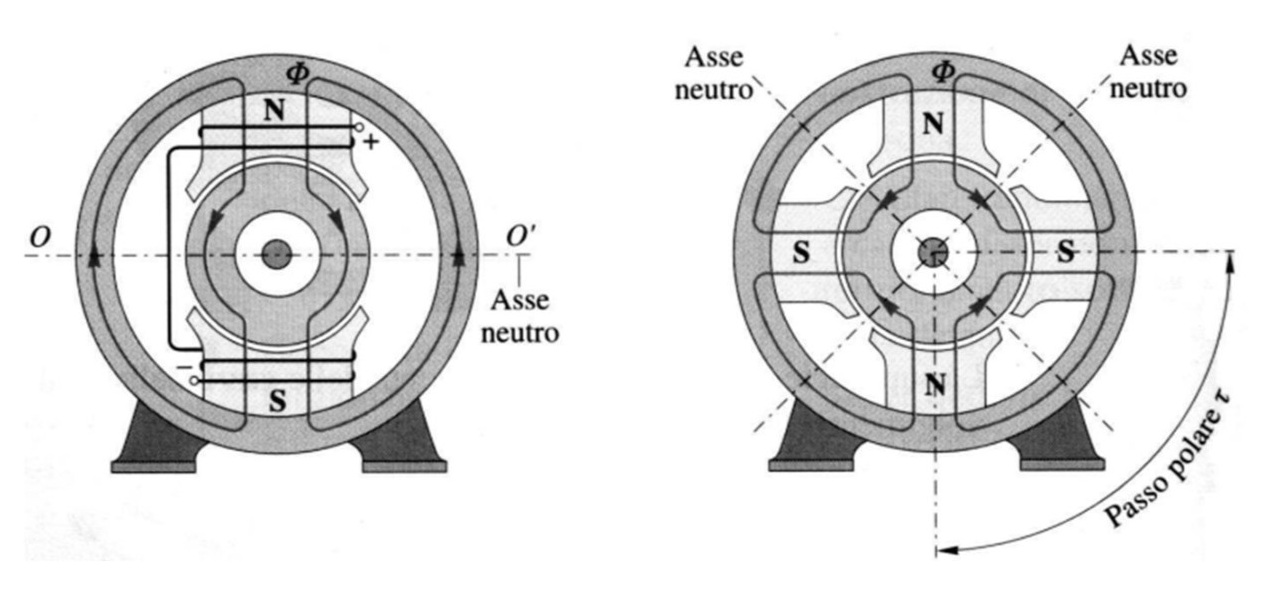
\includegraphics[width=0.55\textwidth]{StatorePoliDC.jpg}
    \caption{Sezione Trasversale Di Un Motore DC Con $p=1$ A Sinistra E Con $p=2$ A Destra, Con Asse Polare Diretto, Asse Neutro E Passo Polare $\tau_p$.}
\end{figure}
Dove:
\begin{itemize}
    \item \textbf{Asse Neutro:} Rappresenta il piano ortogonale all'asse polare delle espansioni polari. È il piano in cui il campo magnetico dello statore si annulla e cambia verso, e dove, idealmente, avviene la commutazione della corrente nelle spire
    \item \textbf{Passo Polare ($\tau_p$):} Rappresenta la distanza angolare espressa in gradi meccanici tra gli assi del baricentro di due poli contigui di segno opposto. In presenza di $2p$ poli, tale ampiezza è pari a:
    \[
        \tau_p = \frac{360^\circ}{2p} = \frac{180^\circ}{p}
    \]
    Per una macchina bipolare ($p=1$) si ha $\tau_p = 180^\circ$ meccanici, mentre per una tetrapolare ($p=2$) risulta $\tau_p = 90^\circ$ meccanici.
\end{itemize}
\newpage

\subsubsection{Rotore E Pacco Lamellare}
È la parte interna rotante vincolata meccanicamente alla struttura esterna mediante cuscinetti.\\
È coassiale allo statore e separata da questo da uno strato di aria di spessore millimetrico, detto \textbf{traferro} (\textit{air gap}). Il rotore è costituito da due componenti principali:
\begin{itemize}
    \item \textbf{Pacco Lamellare:} È il corpo cilindrico fissato sull'albero del rotore, formato da sottili lamine di acciaio al silicio, con spessore compreso tra $0.35\,\si{\milli\meter}$ e $0.5\,\si{\milli\meter}$, isolate elettricamente tra loro mediante strati di vernice o ossido e impilate a formare un cilidro coassiale all'albero. Questa struttura riduce le correnti parassite, limitando le perdite energetiche e il surriscaldamento del rotore.

    \item \textbf{Avvolgimento D'Indotto:} È formato da bobine in rame alloggiate nelle scanalature longitudinali, chiamate \textbf{cave}, ricavate sulla superficie esterna del pacco lamellare. Le bobine sono percorse dalla corrente di armatura $I_a$ che interagendo con il campo magnetico generato dallo statore, produce la forza elettromagnetica responsabile della coppia motrice del rotore.
\end{itemize}
% Immagine Chiarificativa Di Questa Struttura: IndustrialRobotics\Appunti Latex\Images\Lab\Spiegazione Visiva Rotore Brushless DC.png
\begin{figure}[H]
    \centering
    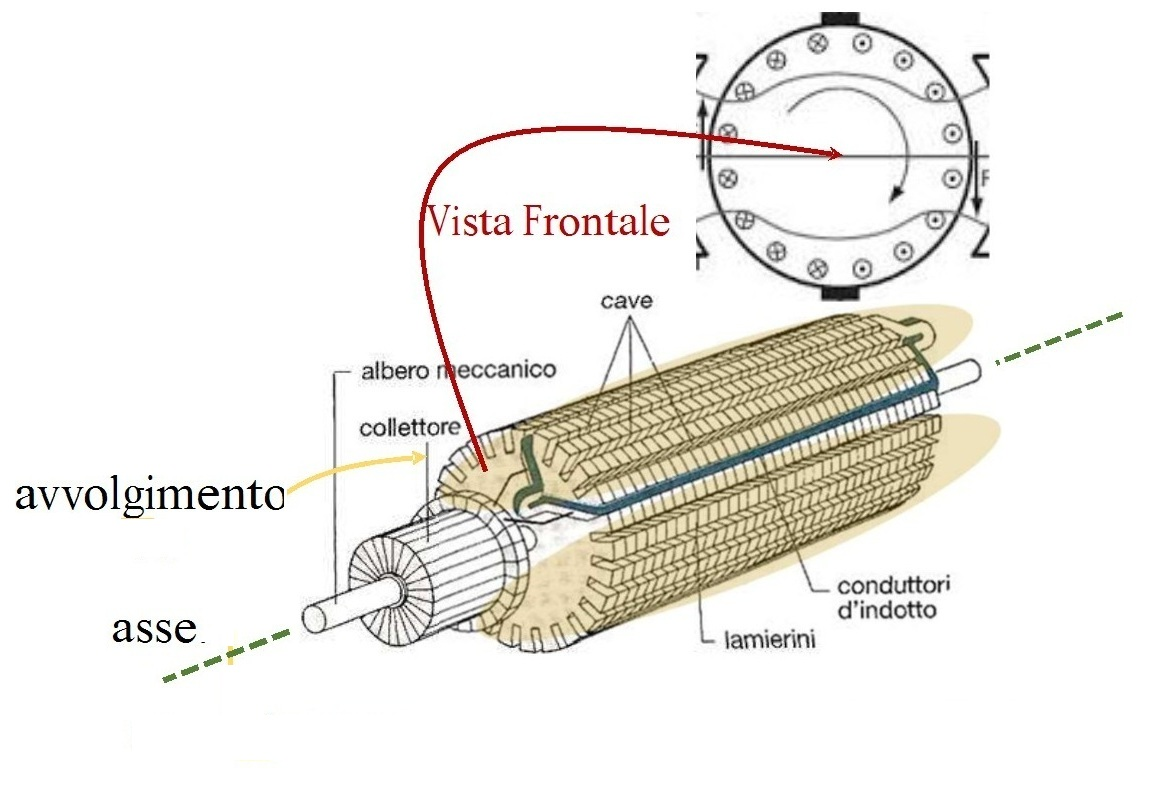
\includegraphics[width=0.35\textwidth]{Rotore.jpg}
    \caption{Pacco Rotorico Di Un Motore DC: Si Notano La Struttura Lamellare, Le Cave Longitudinali Destinate A Ospitare Gli Avvolgimenti Di Indotto E L'Albero Di Trasmissione.}
    \label{fig:rotore}
\end{figure}

\subsubsection{Sistema Collettore-Spazzole E Commutazione}
Il compito principale del sistema Collettore-Spazzole è quello di realizzare la \textbf{commutazione}, ovvero invertire periodicamente il verso della corrente negli avvolgimenti di indotto, in modo da mantenere la coppia sempre nello stesso verso. È costituito da due componenti principali:
\begin{itemize}
    \item \textbf{Collettore A Lamelle} (\textit{commutator}): È una struttura cilindrica fissata direttamente sull'albero del rotore, formata \textbf{lamelle} in rame isolate l'una dall'altra e ognuna collegata a un avvolgimento del rotore (un esempio la bobina $i$ è collegata a due lamelle differenti, da una entra la corrente da una esce)

    \item \textbf{Spazzole} (\textit{brushes}): Sono blocchetti realizzati in grafite o composti di rame e carbone, alloggiati in appositi portaspazzole solidali allo statore e collegate ai poli dell'alimentazione. Vengono premute contro la superficie esterna del collettore tramite molle calibrate, realizzando un contatto strisciante a bassa resistenza ohmica attraverso cui scorre la corrente di armatura $I_a$.
\end{itemize}

\begin{figure}[H]
    \centering
    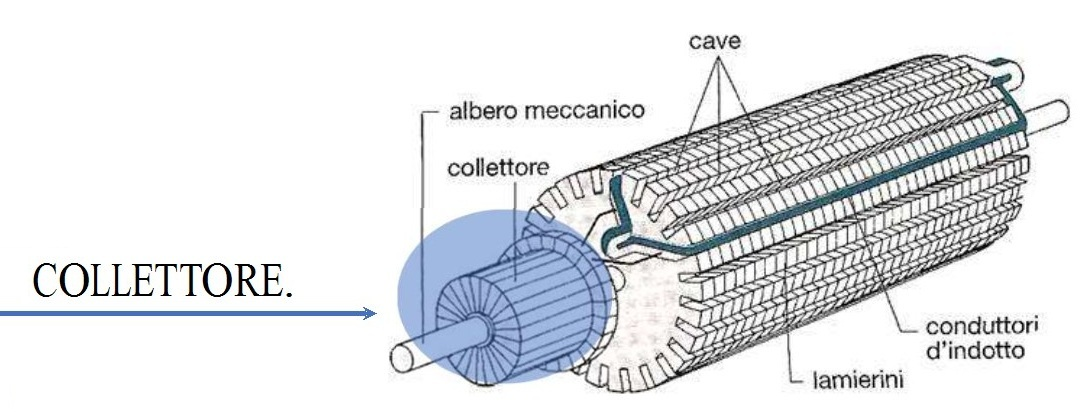
\includegraphics[width=0.4\textwidth]{Collettore.jpg}
    \caption{Dettaglio Del Collettore A Lamelle In Rame Montato Solidale All'Albero Rotante, Con Isolamento Interlamellare In Fogli Di Mica.}
    \label{fig:collettore}
\end{figure}
\newpage
Si utilizza un \textbf{collettore a lamelle}, collegato agli avvolgimenti d'indotto, per invertire periodicamente il verso della corrente nelle bobine del rotore e mantenere la coppia motrice nello stesso verso.

Essendo le lamelle fissate radialmente all'albero, quando l'albero gira, anche le lamelle girano. Ogni lamella è collegata a un estremità delle bobine del rotore. Le spazzole, invece, sono solidali allo statore e rimangono ferme, collegate ai poli dell'alimentazione.

Durante la rotazione del rotore, le spazzole entrano progressivamente in contatto con diverse lamelle, modificando la corrente all'interno del rotore. Quando una spira passa dal lato opposto dell'asse neutro, che idealmente rappresenta il piano in cui il campo magnetico si annulla e cambia verso, le spazzole entrano in contatto con lamelle collegate allo stesso avvolgimento, generando un cortocircuito temporaneo che comporta la \textbf{commutazione} della corrente. \\
A questo punto, la spira entrando nel campo magnetico opposto, avrà la corrente invertita e quindi la forza generata dall'interazione con il campo magnetico sarà nella direzione corretta e di conseguenza la coppia generata avrà il verso corretto per mantenere e non frenare la rotazione

\subsection{Principi Fisici E Modellazione Elettromeccanica}

\subsubsection{Generazione Della Coppia Motrice (Forza Di Lorentz)}
Nei motori \textit{brushed DC} la coppia si genera grazie alla \textbf{forza di Lorentz}. In pratica, considerando un conduttore di lunghezza infinitesima \(d\bm{\ell}\), percorso da una corrente \(I\) e immerso in un campo magnetico \(\bm{B}\), la forza elementare è:
\[
    d\bm{F} = I \, (d\bm{\ell} \times \bm{B})
\]
Per un conduttore rettilineo di lunghezza \(L\), immerso in un campo uniforme, il modulo della forza è:
\[
    F = I L B \sin(\alpha)
\]
dove \(\alpha\) è l'angolo tra la direzione della corrente e quella del campo magnetico.

La forma delle \textbf{espansioni polari} fa sì che, nel traferro, il campo magnetico sia prevalentemente radiale. Poiché i conduttori attivi del rotore sono paralleli all'asse dell'albero, la corrente risulta perpendicolare al campo magnetico, per cui \(\alpha \approx 90^\circ\). La forza assume quindi il valore massimo:
\[
    F = I L B
\]
Consideriamo una singola spira rettangolare del rotore, con lati attivi di lunghezza \(L\) posti a una distanza \(r\) dall'asse di rotazione. Nei due lati attivi le correnti hanno verso opposto e poiché ogni conduttore si trova in prossimità di uno dei poli è immerso in un campo magnetico (di versi opposti tra loro). Sono presenti anche le due testate (materiale conduttivo) che collegano i lati attivi, ma essendo parallele al campo magnetico non contribuiscono alla generazione della coppia.

\begin{figure}[H]
    \centering
    \begin{tikzpicture}[
        scale=1,
        font=\sffamily,
        >=Stealth,
        line width=1.1pt
    ]
        % --- PARAMETRI GEOMETRIA ---
        \def\R{2.0}
        \def\ang{35}

        % Polo Nord
        \draw[fill=poleN!12, draw=poleN, line width=1.3pt]
            (-4.2, -2.1) rectangle (-3.3, 2.1);
        \node[font=\bfseries\small, text=poleN, rotate=90]
            at (-3.75, 0) {POLO N};

        % Polo Sud
        \draw[fill=poleS!12, draw=poleS, line width=1.3pt]
            (3.3, -2.1) rectangle (4.2, 2.1);
        \node[font=\bfseries\small, text=poleS, rotate=-90]
            at (3.75, 0) {POLO S};

        % Campo magnetico nel traferro
        \foreach \y in {-1.2, 0, 1.2} {
            \draw[->, draw=bField, dashed, line width=0.8pt]
                (-3.3, \y) -- (3.3, \y);
        }
        \node[above, font=\footnotesize\bfseries, text=bField]
            at (0, 1.25) {$\bm{B}$};

        % Rotore e assi
        \draw[fill=rotorFill, draw=black!75, line width=1.2pt]
            (0,0) circle (\R);
        \draw[draw=black!35, dashed, line width=0.7pt]
            (-\R-0.3, 0) -- (\R+0.3, 0);
        \draw[draw=black!35, dashed, line width=0.7pt]
            (0, -\R-0.3) -- (0, \R+0.3);

        % Posizioni dei conduttori
        \coordinate (C1) at (\ang:\R);
        \coordinate (C2) at ({180+\ang}:\R);

        % Collegamento schematico della spira
        \draw[draw=black!85, line width=1.4pt] (C2) -- (C1);

        % Raggio e angolo
        \node[above left=1pt, font=\small\bfseries]
            at (\ang:1.0) {$r$};
        \draw[->, draw=black, line width=1pt]
            (0:1.2) arc (0:\ang:1.2);
        \node[right=2pt, font=\small\bfseries]
            at (\ang/2:1.35) {$\theta$};

        % Albero centrale
        \filldraw[fill=black!15, draw=black, line width=1.2pt]
            (0,0) circle (0.32);
        \fill[black] (0,0) circle (2pt);

        % Coppia motrice indicata schematicamente
        \draw[->, line width=1.3pt, draw=black]
            (100:0.6) arc (100:-30:0.6)
            node[pos=0.85, below right=1pt, font=\small\bfseries]
            {$\tau_m$};

        % Conduttore destro: corrente entrante nel piano
        \filldraw[fill=white, draw=black, line width=1.3pt]
            (C1) circle (0.22);
        \draw[line width=1.1pt]
            ([shift={(-0.1,-0.1)}]C1) --
            ([shift={(0.1,0.1)}]C1);
        \draw[line width=1.1pt]
            ([shift={(-0.1,0.1)}]C1) --
            ([shift={(0.1,-0.1)}]C1);
        \node[above right=3pt, font=\small\bfseries]
            at (C1) {$I_a\,(\otimes)$};
        \draw[->, line width=1.8pt, draw=forceColor]
            (C1) -- ++({\ang-90}:1.3)
            node[below right=1pt, font=\bfseries] {$\bm{F}$};

        % Conduttore sinistro: corrente uscente dal piano
        \filldraw[fill=white, draw=black, line width=1.3pt]
            (C2) circle (0.22);
        \fill[black] (C2) circle (2.6pt);
        \node[below left=3pt, font=\small\bfseries]
            at (C2) {$I_a\,(\odot)$};
        \draw[->, line width=1.8pt, draw=forceColor]
            (C2) -- ++({180+\ang-90}:1.3)
            node[above left=1pt, font=\bfseries] {$\bm{F}$};

    \end{tikzpicture}
    \caption{Rappresentazione schematica delle forze agenti sui due lati attivi della spira.}
\end{figure}
\newpage
Applicando il prodotto vettoriale, le forze di Lorentz risultano opposte tra loro e tangenti alla traiettoria circolare. Entrambe producono un momento nello stesso verso rispetto all'asse di rotazione e di consenguenza, la \textbf{coppia totale} generata dalla spira è:
\[
    \tau(\theta) = 2rF\sin(\theta)
\]
Sostituendo \(F = I_a L B\), si ottiene:
\[
    \boxed{\tau(\theta) = 2r I_a L B \sin(\theta)}
\]
dove \(\alpha\) è l'angolo tra la direzione della corrente e quella del campo magnetico. Il fattore \(\sin(\theta)\) descrive la variazione del braccio delle forze durante la rotazione. In particolare:
\begin{itemize}
    \item \textbf{Coppia Massima (\(\theta = 90^\circ\)):} Il braccio delle forze è massimo e vale \(r\).
    \item \textbf{Coppia Nulla (\(\theta = 0^\circ\)):} Il braccio è nullo e le forze non generano un momento risultante attorno all'asse.
\end{itemize}
Una singola spira alimentata in corrente continua sviluppa quindi una coppia che varia con l'angolo di rotazione e presenta posizioni in cui la coppia è nulla. Se il rotore si arresta esattamente in una di queste posizioni, la sola spira potrebbe non generare una coppia iniziale sufficiente a riavviarlo.

Nei motori reali tale discontinuità viene superata adottando commutatori a elevato numero di lamelle (tipicamente $12 \div 48$) e facendo in modo che le spazzole alimentino istante per istante soltanto le bobine che transitano nell'intervallo angolare a rendimento massimo ($\theta \approx 90^\circ$). La coppia complessiva $\tau_m$, risultante dalla sovrapposizione di molteplici contributi sfalsati nello spazio, presenta un profilo temporale quasi costante, riducendo al minimo l'ondulazione residua (\textbf{ripple di coppia}).

\subsubsection{Forza Contro-Elettromotrice E Bilancio Di Armatura}
Quando il rotore è in movimento, i conduttori dell'avvolgimento di indotto ruotano all'interno del campo magnetico generato dallo statore. In base alla \textbf{legge di Faraday-Neumann-Lenz}, questo moto relativo con velocità angolare meccanica $\omega_m$ ($\si{\radian\per\second}$) provoca una variazione nel tempo del flusso magnetico concatenato con le bobine, inducendo una tensione interna nei conduttori.

Questa tensione prende il nome di \textbf{forza contro-elettromotrice (FCEM)}, indicata con $E_a$, poiché, per la legge di Lenz, ha una polarità che si oppone alla tensione di alimentazione esterna $V_a$ che ha generato il movimento. Il valore medio della forza contro-elettromotrice ai morsetti del motore è dato da:
\[
    E_a = K_e \Phi \omega_m
\]
dove:
\begin{itemize}
    \item \textbf{Flusso Magnetico ($\Phi$):} È il flusso magnetico utile per polo presente nel traferro, espresso in Weber ($\si{\weber} = \si{\volt\second}$).
    \item \textbf{Velocità Angolare ($\omega_m$):} È la velocità di rotazione meccanica dell'albero, espressa in $\si{\radian\per\second}$.
    \item \textbf{Costante Elettrica ($K_e$):} È una costante costruttiva che dipende dalla geometria degli avvolgimenti:
    \[
        K_e = \frac{p Z}{2\pi a}
    \]
    in cui $p$ è il numero di coppie polari, $Z$ è il numero totale di conduttori attivi del rotore e $2a$ indica il numero di vie di corrente in parallelo formate dall'avvolgimento.
\end{itemize}

Per descrivere il comportamento elettrico del motore a regime stazionario, possiamo scrivere l'equazione di bilancio delle tensioni nel circuito di armatura. Trascurando la piccola caduta di tensione dovuta al contatto sulle spazzole (solitamente intorno a $1 \div 2\,\si{\volt}$), la tensione continua di alimentazione $V_a$ ($\si{\volt}$) si ripartisce tra la caduta resistiva sugli avvolgimenti e la forza contro-elettromotrice:
\[
    V_a = R_a I_a + E_a
\]
dove $R_a$ ($\si{\ohm}$) rappresenta la resistenza ohmica complessiva degli avvolgimenti di indotto. Esplicitando la corrente di armatura $I_a$, si ottiene:
\[
    \boxed{I_a = \frac{V_a - E_a}{R_a} = \frac{V_a - K_e \Phi \omega_m}{R_a}}
\]
Questa relazione mostra chiaramente come il motore possieda una sorta di \textbf{autoregolazione naturale} che lega la parte meccanica a quella elettrica. In particolare, si possono distinguere tre situazioni tipiche:
\begin{itemize}
    \item \textbf{Condizione Di Avviamento ($\omega_m = 0$):} All'istante iniziale il rotore è fermo, quindi non c'è variazione di flusso e la forza contro-elettromotrice è nulla ($E_a = 0$). La corrente assorbita, detta \textbf{corrente di spunto}, è limitata unicamente dalla resistenza degli avvolgimenti:
    \[
        I_{\text{spunto}} = \frac{V_a}{R_a}
    \]
    Poiché nei motori la resistenza $R_a$ è progettata per essere molto bassa (spesso inferiore a $1\,\si{\ohm}$ per ridurre le perdite per effetto Joule), la corrente di spunto può raggiungere valori da $5$ a $10$ volte superiori alla corrente nominale. Per questo motivo è spesso necessario utilizzare sistemi di controllo che applichino la tensione gradualmente durante l'avvio.

    \item \textbf{Funzionamento A Regime ($\omega_m > 0$):} Man mano che il rotore accelera, la velocità $\omega_m$ aumenta e con essa cresce anche la tensione $E_a$. Di conseguenza, la differenza di potenziale netta $(V_a - E_a)$ diminuisce, facendo scendere progressivamente la corrente $I_a$. Il motore accelera fino a raggiungere una velocità di equilibrio, in cui la coppia generata dal rotore è uguale alla coppia generata dal carico.

    \item \textbf{Variazione Del Carico Meccanico:} Se durante il funzionamento viene applicato un carico maggiore all'albero, il rotore tende inizialmente a rallentare. La diminuzione della velocità $\omega_m$ fa abbassare subito la forza contro-elettromotrice $E_a$, facendo aumentare la differenza $(V_a - E_a)$ e, di conseguenza, la corrente $I_a$ che circola nel rotore. L'aumento di corrente permette al motore di sviluppare spontaneamente una coppia motrice più elevata, necessaria per contrastare il nuovo carico e stabilizzarsi su un nuovo punto di equilibrio.
\end{itemize}

\subsubsection{Bilancio Di Potenza Ed Equivalenza Delle Costanti \texorpdfstring{$K_e$}{Ke} E \texorpdfstring{$K_t$}{Kt}}
La coppia totale $\tau_m$ ($\si{\newton\meter}$) sviluppata dal rotore è direttamente proporzionale al flusso magnetico $\Phi$ e alla corrente di armatura $I_a$:
\[
    \tau_m = K_t \Phi I_a
\]
dove $K_t$ prende il nome di \textbf{costante di coppia} del motore.

Supponendo un contesto ideale, ovvero senza attriti e perdite, in regime stazionario tutta la potenza elettromagnetica viene convertita in potenza meccanica all'albero. In questo contesto quindi, si può uguagliare la potenza elettromagnetica $P_{\text{em}}$ con la potenza meccanica $P_{\text{mec}}$:
\begin{align*}
    P_{\text{em}} &= P_{\text{mec}}\\
    E_{a} I_{a} &= \tau_{m} \omega_{m}\\
    (K_e \Phi \omega_m) I_a &= (K_t \Phi I_a) \omega_m
\end{align*}
Semplificando in entrambi i membri i termini comuni $(\Phi I_a \omega_m)$, si giunge a una relazione fondamentale:
\[
    \boxed{K_e = K_t} \quad \left[\si{\volt\second\per\radian} \equiv \si{\newton\meter\per\ampere}\right]
\]
Questo risultato dimostra che, esprimendo la velocità angolare in $\si{\radian\per\second}$, \textbf{la costante elettrica e la costante di coppia assumono esattamente lo stesso valore numerico} e sono dimensionalmente equivalenti.

Nella pratica industriale, tuttavia, i cataloghi dei costruttori esprimono spesso la costante $K_e$ in unità pratiche non appartenenti al Sistema Internazionale, come i $\si{\milli\volt}$ per giro al minuto ($\si{\milli\volt\per\rpm}$). Per riportare il valore dei datasheet all'unità standard ($\si{\volt\second\per\radian}$), è sufficiente applicare il fattore di conversione legato alla velocità angolare:
\[
    K_e \left[\si{\volt\second\per\radian}\right] = \frac{30}{\pi \cdot 1000} \, K_e \left[\frac{\si{\milli\volt}}{\si{rpm}}\right]
\]
\newpage

\subsection{Configurazioni Circuitali E Caratteristiche Meccaniche}

\subsubsection{Servomotori A Magneti Permanenti}
Nei servomotori a \textbf{Magneti Permanenti}, il flusso magnetico $\Phi$ nel traferro è costante e quindi si può inglobare questo parametro nelle costanti globali di macchina definendo
\[
    K'_{E} = K_e \Phi \qquad K'_{T} = K_t \Phi
\]
E di conseguenza le equazioni di forza contro elettromotrice e di coppia del rotore diventano:
\begin{align*}
    E_a     &= K'_{E} \cdot \omega_m\\
    \tau_m  &= K'_{T} \cdot I_a
\end{align*}
Da questo risulta che la coppia $\tau_m$ dipende solo dalla corrente di armatura $I_{a}$ mentre la tensione regola solo la velocità angolare $\omega_m$

Nei \textbf{Motori A Eccitazione Separata}, i circuiti dello statore e del rotore dipendono da due alimentazioni indipendenti statorico e rotorico fanno capo a due alimentatori indipendenti a tensione $V_{\text{ecc}}$ e $V_a$.

Nei servomotori con \textbf{Avvolgimento Di Eccitazione}, la relazione tra la coppia e velocità angolare dipende dalla connessione tra il circuito dello statore e il circuito del rotore

\subsubsection{Motore Con Eccitazione In Parallelo (Shunt)}
Nel \textbf{Motore Shunt} (O Con Eccitazione In Derivazione) il circuito di eccitazione e il circuito di armatura sono collegati in parallelo.

\begin{figure}[H]
    \centering
    \scalebox{0.8}{%
        \begin{tikzpicture}[
            line width=1pt,
            font=\sffamily,
            terminal/.style={circle, draw=accent, fill=white, inner sep=1.8pt, line width=1.2pt},
            brush/.style={fill=accent, draw=accent, rounded corners=0.4pt},
            wire/.style={draw=accent, line cap=round, line join=round},
            junc/.style={circle, fill=accent, inner sep=1.5pt}
        ]

            % --- Coordinate Griglia (Identiche per entrambi gli schemi) ---
            \coordinate (VinTop) at (0, 2.8);
            \coordinate (VinBot) at (0, 0);
            \coordinate (JuncTop) at (2.6, 2.8);
            \coordinate (JuncBot) at (2.6, 0);
            \coordinate (F1) at (2.6, 2.15);
            \coordinate (F2) at (2.6, 0.65);
            \coordinate (ArmCenter) at (5.0, 1.4);

            % --- Morsetti Ingresso DC ---
            \node[terminal] (in+) at (VinTop) {};
            \node[terminal] (in-) at (VinBot) {};
            \node[left=3pt of in+, font=\bfseries] {$+$};
            \node[left=3pt of in-, font=\bfseries] {$-$};

            % Indicazione Tensione DC (spazio pulito, nessun contatto con le etichette)
            \draw[{Latex[length=3.5pt]}-{Latex[length=3.5pt]}, draw=subtext, dashed]
                ($(VinTop)+(0.45, -0.15)$) -- ($(VinBot)+(0.45, 0.15)$)
                node[midway, fill=white, inner sep=1.5pt, font=\scriptsize\bfseries, text=subtext] {$V_{\mathrm{DC}}$};

            % --- Ramo 1: Avvolgimento Statore (Shunt / Parallelo) ---
            \draw[wire] (in+) -- (5.0, 2.8);
            \draw[wire] (in-) -- (5.0, 0);

            \node[junc] at (JuncTop) {};
            \node[junc] at (JuncBot) {};
            \draw[wire] (JuncTop) -- (F1);
            \draw[wire] (F2) -- (JuncBot);

            % Spire Statore (4 archi ben raccordati)
            \draw[wire, line width=1.2pt, color=primary]
                (F1) arc[start angle=90, end angle=-90, radius=0.1875]
                    arc[start angle=90, end angle=-90, radius=0.1875]
                    arc[start angle=90, end angle=-90, radius=0.1875]
                    arc[start angle=90, end angle=-90, radius=0.1875] -- (F2);

            % Etichette Statore
            \node[right=4pt, text=accent, font=\scriptsize\bfseries, align=center] at (1, 1.4) {Avv.\\Statore};
            \node[left=3pt, text=subtext, font=\tiny\bfseries] at (F1) {F1};
            \node[left=3pt, text=subtext, font=\tiny\bfseries] at (F2) {F2};

            % --- Ramo 2: Rotore (Indotto) ---
            \draw[wire] (5.0, 2.8) -- ($(ArmCenter)+(0, 0.92)$);
            \draw[wire] ($(ArmCenter)+(0, -0.92)$) -- (5.0, 0);

            % Cerchio Rotore
            \draw[line width=1.3pt, draw=primary, fill=rotorFill]
                (ArmCenter) circle (0.75);
            \node[font=\large\bfseries, text=primary] at (ArmCenter) {A};

            % Spazzole
            \draw[brush] ($(ArmCenter)+(-0.18, 0.75)$) rectangle ($(ArmCenter)+(0.18, 0.92)$);
            \draw[brush] ($(ArmCenter)+(-0.18, -0.75)$) rectangle ($(ArmCenter)+(0.18, -0.92)$);

            % Morsetti Spazzole
            \node[left=4pt, text=subtext, font=\tiny\bfseries] at ($(ArmCenter)+(-0.18, 0.83)$) {A1};
            \node[left=4pt, text=subtext, font=\tiny\bfseries] at ($(ArmCenter)+(-0.18, -0.83)$) {A2};

            % Etichetta Rotore
            \node[right=4pt, text=accent, font=\scriptsize\bfseries, align=center] at (5.6, 1.4) {Avv.\\Rotore};

        \end{tikzpicture}%
    }
\end{figure}
Al fine di minimizzare la corrente assorbita per la generazione del campo magnetico dello statore, si deve avere che $I_{acc} \ll I_{a}$. Per questo motivo, per gli avvolgimenti, in questo caso, si utilizzano delle spire sottili e quindi che hanno una resistenza $R_{ecc}$ elevata, di conseguenza la corrente di eccitazione, data da $I_{\text{ecc}} = V / R_{\text{ecc}}$ sarà ridotta e produrrà un flusso magnetico costante e privo di oscillazioni.

Per ottenere la caratteristica meccanica a regime stazionario, si considera l'equazione alla maglia d'armatura $V = E_a + R_a I_a$. Andando a sostituire l'equazione della corrente ricavata tramite l'equazione della coppia $\tau_{m}$ si ottiene:
\[
    V = K_e \Phi \omega_m + R_a \left(\frac{\tau_m}{K_t \Phi}\right)
\]
Da cui, si ricava l'\textbf{equazione caratteristica del motore Shunt}
\begin{align*}
    K_e \Phi \omega_m &= V - \frac{R_a}{K_t \Phi} \tau_m\\
    \omega_m(\tau_m) &= \frac{V}{K_e \Phi} - \frac{R_a}{(K_t \Phi)(K_e \Phi)} \cdot \tau_m
\end{align*}
Questa equazione desrive una retta in funzione della coppia $\tau_{m}$ nel piano $(\tau_m, \omega_m)$. Si nota che
\begin{itemize}
    \item \textbf{Per $\tau_m = 0$:} Si ottiene la \textit{Velocità A Vuoto} che corrisponde alla velocità del motore senza il carico ed è:
    \[
        \omega_0 = \frac{V}{K_e \Phi}
    \]
    \item \textbf{Per $\tau_m \ne 0$:} Il valore della velocità dipende dal fattore $\frac{R_a}{(K_t \Phi)(K_e \Phi)}$, ma essendo la resistenza di armatura $R_{a}$ un valore non troppo elevato, questo valore non riduce di tanto il valore della velocità a vuoto
\end{itemize}
Per questi motivi, la caratteristica del motore Shunt è detta \textbf{rigida}, perchè il calo della velocità tra a vuoto e con carico è limitata (entro il $3\% \div 6\%$)
\newpage

\subsubsection{Motore Con Eccitazione In Serie}
Nel \textbf{Motore In Serie} il circuito di eccitazione e il circuito di armatura sono collegati in serie, e di conseguenza si ha che $I_{ecc} = I_{a} = I$

\begin{figure}[H]
    \centering
    \scalebox{0.8}{%
        \begin{tikzpicture}[
            line width=1.1pt,
            font=\sffamily,
            terminal/.style={circle, draw=accent, fill=white, inner sep=1.8pt, line width=1.2pt},
            brush/.style={fill=accent, draw=accent, rounded corners=0.4pt},
            wire/.style={draw=accent, line cap=round, line join=round}
        ]

            % --- Coordinate Griglia (Identiche allo Shunt) ---
            \coordinate (VinTop) at (0, 2.8);
            \coordinate (VinBot) at (0, 0);
            \coordinate (S1) at (1.6, 2.8);
            \coordinate (S2) at (3.6, 2.8);
            \coordinate (ArmCenter) at (5.0, 1.4);

            % --- Morsetti Ingresso DC ---
            \node[terminal] (in+) at (VinTop) {};
            \node[terminal] (in-) at (VinBot) {};
            \node[left=3pt of in+, font=\bfseries] {$+$};
            \node[left=3pt of in-, font=\bfseries] {$-$};

            % Indicazione Tensione DC
            \draw[{Latex[length=3.5pt]}-{Latex[length=3.5pt]}, draw=subtext, dashed]
                ($(VinTop)+(0.45, -0.15)$) -- ($(VinBot)+(0.45, 0.15)$)
                node[midway, fill=white, inner sep=1.5pt, font=\scriptsize\bfseries, text=subtext] {$V_{\mathrm{DC}}$};

            % --- Avvolgimento Statore (Serie) ---
            \draw[wire] (in+) -- (S1);

            \draw[wire, line width=1.2pt, color=primary]
                (S1) arc[start angle=180, end angle=0, radius=0.333]
                    arc[start angle=180, end angle=0, radius=0.333]
                    arc[start angle=180, end angle=0, radius=0.333] -- (S2);

            % Etichette Statore
            \node[right=4pt, text=accent, font=\scriptsize\bfseries, align=center] at (1.75, 3.5) {Avv.\\Statore};
            \node[below=3pt, text=subtext, font=\tiny\bfseries] at (S1) {S1};
            \node[below=3pt, text=subtext, font=\tiny\bfseries] at (S2) {S2};

            % --- Collegamento verso il Rotore ---
            \draw[wire] (S2) -- (5.0, 2.8) -- ($(ArmCenter)+(0, 0.92)$);
            \draw[wire] ($(ArmCenter)+(0, -0.92)$) -- (5.0, 0) -- (in-);

            % --- Cerchio Rotore (Identico allo Shunt) ---
            \draw[line width=1.3pt, draw=primary, fill=rotorFill]
                (ArmCenter) circle (0.75);
            \node[font=\large\bfseries, text=primary] at (ArmCenter) {A};

            % Spazzole
            \draw[brush] ($(ArmCenter)+(-0.18, 0.75)$) rectangle ($(ArmCenter)+(0.18, 0.92)$);
            \draw[brush] ($(ArmCenter)+(-0.18, -0.75)$) rectangle ($(ArmCenter)+(0.18, -0.92)$);

            % Morsetti Spazzole
            \node[left=4pt, text=subtext, font=\tiny\bfseries] at ($(ArmCenter)+(-0.18, 0.83)$) {A1};
            \node[left=4pt, text=subtext, font=\tiny\bfseries] at ($(ArmCenter)+(-0.18, -0.83)$) {A2};

            % Etichetta Rotore
            \node[right=4pt, text=accent, font=\scriptsize\bfseries, align=center] at (5.6, 1.4) {Avv.\\Rotore};

        \end{tikzpicture}%
    }
\end{figure}

poiché la corrente che scorre in entrambi i circuiti e uguale, si deve fare in modo che la corrente che nel circuito di generazione del campo magnetico non ci siano perdite e che $R_{ecc} \ll R_{a}$ e per questo motivo, le spire degli avvolgimenti dello statore hanno una sezione elevata per ridurre la resistenza

Per polo. il flusso magnetico risulta proporzionale alla corrente e quindi poiché la corrente che scorre in entrambi i circuiti è uguale:
\[
    \Phi = c_f \cdot I_a
\]
Dove $c_f$ è la costante di proporzionalità del circuito magnetico. Sostituendo nell'equazione della coppia $\tau_{m}$ si ottiene
\[
    \tau_m = K_t \cdot (c_f \cdot I_a) \cdot I_a = K_t \, c_f \cdot I_a^2
\]
Quindi, nel motore in serie \underline{la coppia del rotore è proporzionale al quadrato della corrente}, e isolando $I_{a}$ si ottiene:
\[
    I_a = \sqrt{\frac{\tau_m}{K_t c_f}}
\]
L'equazione di bilancio delle tensioni in questo caso sarà
\begin{align*}
    V &= E_a + (R_a + R_{\text{ecc}}) \cdot I_a =\\
    &= K_e (c_f I_a) \omega_m + (R_a + R_{\text{ecc}}) \cdot I_a
\end{align*}
Sostituendo $I_a$ si ottiene
\[
    V = K_e c_f \sqrt{\frac{\tau_m}{K_t c_f}} \cdot \omega_m + (R_a + R_{\text{ecc}}) \cdot \sqrt{\frac{\tau_m}{K_t c_f}}
\]
Isolando il termine dipendente da $\omega_m$:
\begin{align*}
    K_e c_f \sqrt{\frac{\tau_m}{K_t c_f}} \cdot \omega_m &= V - (R_a + R_{\text{ecc}}) \cdot \sqrt{\frac{\tau_m}{K_t c_f}}\\
    \omega_m &= \frac{V}{K_e c_f \sqrt{\frac{\tau_m}{K_t c_f}}} - \frac{(R_a + R_{\text{ecc}}) \cdot \sqrt{\frac{\tau_m}{K_t c_f}}}{K_e c_f \sqrt{\frac{\tau_m}{K_t c_f}}}\\
    \omega_m &= \frac{V}{K_e c_f \sqrt{\frac{\tau_m}{K_t c_f}}} - \frac{(R_a + R_{\text{ecc}})}{K_e c_f}
\end{align*}
Per quanto riguarda il primo termine:
\[
    \frac{V}{K_e c_f \sqrt{\frac{\tau_m}{K_t c_f}}} = \frac{V}{K_e c_f \frac{\sqrt{\tau_m}}{K_t c_f}} = \frac{V \sqrt{K_t c_f}}{K_e c_f \sqrt{\tau_m}}  = \frac{V \sqrt{K_t} \sqrt{c_f}}{K_e c_f \sqrt{\tau_m}}
\]
poiché, in condizioni ideali $K_{t} = K_{e}$ e la radice è uguale ad elevare a $\frac{1}{2}$, si ottiene
\[
    = \frac{V K_{e}^{\frac{1}{2}} c_{f}^{\frac{1}{2}}}{K_e c_f \sqrt{\tau_m}} = \frac{V K_{e}^{-\frac{1}{2}} c_{f}^{-\frac{1}{2}}}{ \sqrt{\tau_m}} = \frac{V}{\sqrt{K_e c_f}} \cdot \frac{1}{\sqrt{\tau_m}}
\]
E sostituendo nell'equazione di $\omega_{m}$ si ottiene l'\textbf{equazione caratteristica del motore in serie:}
\[
    \omega_m(\tau_m) = \frac{V}{\sqrt{K_e c_f}} \cdot \frac{1}{\sqrt{\tau_m}} - \frac{R_a + R_{\text{ecc}}}{K_e c_f}
    \label{eq:caratteristica_serie}
\]
Questa equazione descrive una curva iperbolica in funzione della coppia $\tau_{m}$ nel piano $(\tau_m, \omega_m)$. Si nota che

\begin{itemize}
    \item \textbf{Per $\omega_m = 0$:} Si ha un elevata coppia di spunto, poiché non essendoci forza contro elettromotrice, la corrente di armatura assume il valore massimo e si ottiene una coppia molto elevata
    \item \textbf{Per $\tau_{m} \approx 0$:} Si ha un elevata velocità angolare. Fisicamente quando diminuisce il carico, diminuisce anche la corrente di armatura $I_a$ e di conseguenza anche il flusso magnetico (che è proporzionale a quest'ultima) e quindi, per generare la forza contro elettromotrice necessaria a bilanciare la tensione di alimentazione, il motore deve per forza aumentare la velocità angolare, raggiungendo idealmente velocità infinite che possono causare danni fisici al motore. Per questo motivo, si deve evitare di avviare a vuoto i motori in serie, oppure prevedere delle contromisure per evitare che il motore si rompa
\end{itemize}

\subsubsection{Motore A Eccitazione Composta (Compound)}
Nel \textbf{Motore Compound} (o a eccitazione composta) si combinano le proprietà del \textit{motore Shunt} e del \textit{motore Serie}. In questa configurazione, su ciascuna \textbf{espansione polare} dello statore sono alloggiati due distinti avvolgimenti:
\begin{itemize}
    \item un avvolgimento a filo sottile con molte spire (avvolgimento derivato o \textit{shunt}), collegato in parallelo al circuito di armatura;
    \item un avvolgimento a filo di sezione elevata con poche spire (avvolgimento serie), collegato in serie al circuito di armatura.
\end{itemize}

\begin{figure}[H]
    \centering
    \scalebox{0.8}{%
        \begin{tikzpicture}[
            line width=1.1pt,
            font=\sffamily,
            terminal/.style={circle, draw=accent, fill=white, inner sep=1.8pt, line width=1.2pt},
            brush/.style={fill=accent, draw=accent, rounded corners=0.4pt},
            wire/.style={draw=accent, line cap=round, line join=round},
            junc/.style={circle, fill=accent, inner sep=1.5pt}
        ]

            % --- Coordinate Griglia (Distanziate per dare respiro a V_DC) ---
            \coordinate (VinTop) at (0, 2.8);
            \coordinate (VinBot) at (0, 0);
            \coordinate (JuncTop) at (2.4, 2.8);
            \coordinate (JuncBot) at (2.4, 0);
            \coordinate (F1) at (2.4, 2.15);
            \coordinate (F2) at (2.4, 0.65);
            \coordinate (S1) at (3.2, 2.8);
            \coordinate (S2) at (4.8, 2.8);
            \coordinate (ArmCenter) at (6.0, 1.4);

            % --- Morsetti Ingresso DC ---
            \node[terminal] (in+) at (VinTop) {};
            \node[terminal] (in-) at (VinBot) {};
            \node[left=3pt of in+, font=\bfseries] {$+$};
            \node[left=3pt of in-, font=\bfseries] {$-$};

            % Indicazione Tensione DC
            \draw[{Latex[length=3.5pt]}-{Latex[length=3.5pt]}, draw=subtext, dashed]
                ($(VinTop)+(0.45, -0.15)$) -- ($(VinBot)+(0.45, 0.15)$)
                node[midway, fill=white, inner sep=1.5pt, font=\scriptsize\bfseries, text=subtext] {$V_{\mathrm{DC}}$};

            % --- Bus Primario e Ramo Derivato (Shunt: F1-F2) ---
            \draw[wire] (in+) -- (S1);
            \draw[wire] (in-) -- (6.0, 0);

            \node[junc] at (JuncTop) {};
            \node[junc] at (JuncBot) {};
            \draw[wire] (JuncTop) -- (F1);
            \draw[wire] (F2) -- (JuncBot);

            % Spire Avvolgimento Shunt
            \draw[wire, line width=1.2pt, color=primary]
                (F1) arc[start angle=90, end angle=-90, radius=0.1875]
                    arc[start angle=90, end angle=-90, radius=0.1875]
                    arc[start angle=90, end angle=-90, radius=0.1875]
                    arc[start angle=90, end angle=-90, radius=0.1875] -- (F2);

            \node[left=3pt, text=subtext, font=\tiny\bfseries] at (F1) {F1};
            \node[left=3pt, text=subtext, font=\tiny\bfseries] at (F2) {F2};
            \node[left=6pt, text=accent, font=\scriptsize\bfseries, align=center] at (2.6, 1.4) {Avv.\\Shunt};

            % --- Ramo Serie (S1-S2) ---
            \draw[wire, line width=1.2pt, color=primary]
                (S1) arc[start angle=180, end angle=0, radius=0.266]
                    arc[start angle=180, end angle=0, radius=0.266]
                    arc[start angle=180, end angle=0, radius=0.266] -- (S2);

            \node[below=3pt, text=subtext, font=\tiny\bfseries] at (S1) {S1};
            \node[below=3pt, text=subtext, font=\tiny\bfseries] at (S2) {S2};
            \node[above=4pt, text=accent, font=\scriptsize\bfseries, align=center] at (4.0, 3.2) {Avv. Serie};

            % --- Ramo Rotore (Indotto) ---
            \draw[wire] (S2) -- (6.0, 2.8) -- ($(ArmCenter)+(0, 0.92)$);
            \draw[wire] ($(ArmCenter)+(0, -0.92)$) -- (6.0, 0);

            % Cerchio Rotore
            \draw[line width=1.3pt, draw=primary, fill=rotorFill]
                (ArmCenter) circle (0.75);
            \node[font=\large\bfseries, text=primary] at (ArmCenter) {A};

            % Spazzole
            \draw[brush] ($(ArmCenter)+(-0.18, 0.75)$) rectangle ($(ArmCenter)+(0.18, 0.92)$);
            \draw[brush] ($(ArmCenter)+(-0.18, -0.75)$) rectangle ($(ArmCenter)+(0.18, -0.92)$);

            % Morsetti Spazzole
            \node[left=4pt, text=subtext, font=\tiny\bfseries] at ($(ArmCenter)+(-0.18, 0.83)$) {A1};
            \node[left=4pt, text=subtext, font=\tiny\bfseries] at ($(ArmCenter)+(-0.18, -0.83)$) {A2};
            \node[right=4pt, text=accent, font=\scriptsize\bfseries, align=center] at (6.6, 1.4) {Avv.\\Rotore};

        \end{tikzpicture}%
    }
    \caption{Schema Circuitale Del Motore Dc A Eccitazione Composta (Compound).}
\end{figure}

Il flusso complessivo per polo è la somma (nella configurazione additiva standard) della quota costante $\Phi_{\text{sh}}$ prodotta dalla bobina shunt e della quota variabile $\Phi_{\text{se}} = c_s I_a$ prodotta dalla bobina serie:
\[
    \Phi_{\text{tot}} = \Phi_{\text{sh}} + c_s I_a
\]
In questo modo si ottiene un comportamento ottimizzato:
\begin{itemize}
    \item \textbf{All'avvio O Per Carichi Elevati:} La corrente di armatura $I_a$ che transita nella bobina serie incrementa notevolmente il flusso $\Phi_{\text{tot}}$, generando una coppia di spunto sensibilmente maggiore rispetto a un equivalente motore Shunt puro.
    \item \textbf{A vuoto O Per Distacco Improvviso Del Carico:} Al tendere di $\tau_m \to 0$, la corrente $I_a$ si azzera e il contributo serie svanisce, ma permane il flusso base $\Phi_{\text{sh}}$ imposto dall'avvolgimento in parallelo; la velocità a vuoto converge quindi stabilmente a un valore finito $\omega_0 = V / (K_e \Phi_{\text{sh}})$, eliminando alla radice il rischio di fuga e danneggiamento meccanico tipico del motore Serie.
\end{itemize}
\newpage

\subsubsection{Confronto Tra Configurazioni}
Il grafico confronta le caratteristiche meccaniche $\omega_m(\tau_m)$ delle tre configurazioni descritte.

\begin{figure}[H]
    \centering
    \scalebox{0.88}{%
        \begin{tikzpicture}[
            font=\sffamily,
            >=Stealth,
            line cap=round,
            line join=round
        ]
            % --- Griglia di Sfondo ---
            \draw[step=1cm, draw=subtext!20, line width=0.5pt] (0,0) grid (8.5, 5.5);

            % --- Assi Cartesiani ---
            \draw[->, line width=1.1pt, draw=accent] (0,0) -- (9.2,0)
                node[below=4pt, anchor=north east, font=\bfseries] {Coppia $\tau_m$ [$\mathrm{N\cdot m}$]};
            \draw[->, line width=1.1pt, draw=accent] (0,0) -- (0,5.8)
                node[above=4pt, anchor=south west, font=\bfseries] {Velocità $\omega_m$ [$\mathrm{rad/s}$]};

            \node[below left=2pt, font=\small\bfseries, text=subtext] at (0,0) {0};

            % --- 1. SHUNT (Caratteristica dura: retta a debole pendenza) ---
            \draw[line width=1.6pt, color=primary]
                (0, 4.3) -- (8.2, 3.4);

            % --- 2. COMPOUND (Caratteristica intermedia) ---
            \draw[line width=1.6pt, color=measGreen]
                plot[domain=0:8.2, samples=80, smooth] (\x, {4.9 - 0.45*\x - 0.012*\x^2});

            % --- 3. SERIE (Caratteristica elastica: iperbolica) ---
            \draw[line width=1.6pt, color=actRed]
                plot[domain=0.55:8.2, samples=100, smooth] (\x, {0.35 + 2.75/(\x^0.8)});

            % Punti a vuoto
            \fill[primary] (0, 4.3) circle (2.2pt) node[left=3pt, font=\footnotesize\bfseries] {$\omega_{0,\text{sh}}$};
            \fill[measGreen] (0, 4.9) circle (2.2pt) node[left=3pt, font=\footnotesize\bfseries] {$\omega_{0,\text{comp}}$};

            % Fuga a vuoto Serie
            \draw[->, line width=1pt, draw=actRed, dashed]
                (0.65, 4.7) -- (0.65, 5.6)
                node[right=3pt, font=\scriptsize\bfseries, text=actRed, align=left] {Pericolo di fuga\\a vuoto ($\tau_m \to 0$)};

            % --- Legenda Esterna a Destra Fuori dal Piano Cartesiano ---
            \node[draw=subtext!35, fill=white, rounded corners=3pt, inner sep=7pt, anchor=west]
                at (9.6, 3.2) {
                \begin{tabular}{l l}
                    \tikz\draw[line width=1.6pt, color=primary] (0,0) -- (0.55,0); & \textbf{\textcolor{primary}{Shunt}} (Rigida) \\[4pt]
                    \tikz\draw[line width=1.6pt, color=measGreen] (0,0) -- (0.55,0); & \textbf{\textcolor{measGreen}{Compound}} (Intermedia) \\[4pt]
                    \tikz\draw[line width=1.6pt, color=actRed] (0,0) -- (0.55,0); & \textbf{\textcolor{actRed}{Serie}} (Elastica)
                \end{tabular}
            };
        \end{tikzpicture}%
    }
    \caption{Confronto Caratteristiche Meccaniche $\omega_m(\tau_m)$ Per Motori Dc Con Eccitazione Shunt, Compound E Serie.}
\end{figure}

Nella tabella vengono riassunti i parametri analitici e le proprietà operative fondamentali delle tre tipologie di motore a corrente continua.

\begin{table}[H]
    \centering
    \renewcommand{\arraystretch}{1.5}
    \scalebox{0.75}{%
    \begin{tabular}{l l l l}
        \toprule
        \textbf{Configurazione} &
        \textbf{Equazione Caratteristica $\bm{\omega_m(\tau_m)}$} &
        \textbf{Coppia Di Spunto} &
        \textbf{Velocità A Vuoto $\bm{\omega_0}$} \\ % <-- Mancava questo \\
        \midrule
        \textbf{\textcolor{primary}{Shunt}} (Parallelo) &
        $\displaystyle \omega_m = \frac{V}{K_e \Phi} - \frac{R_a}{K_t K_e \Phi^2}\,\tau_m$ &
        Media ($\tau_m \propto I_a$) &
        $\displaystyle \frac{V}{K_e \Phi}$ (Finita) \\
        \addlinespace[10pt]
        \textbf{\textcolor{measGreen}{Compound}} (Composto) &
        $\displaystyle \omega_m \approx \frac{V}{K_e \Phi_{\text{tot}}} - \frac{R_a + R_{\text{se}}}{K_t K_e \Phi_{\text{tot}}^2}\,\tau_m$ &
        Elevata &
        $\displaystyle \frac{V}{K_e \Phi_{\text{sh}}}$ (Finita e sicura) \\
        \addlinespace[10pt]
        \textbf{\textcolor{actRed}{Serie}} &
        $\displaystyle \omega_m = \frac{V}{\sqrt{K_e K_t c_f}}\,\frac{1}{\sqrt{\tau_m}} - \frac{R_a + R_{\text{se}}}{K_e K_t c_f}$ &
        Molto Elevata ($\tau_m \propto I_a^2$) &
        $\to \infty$ \textbf{\textcolor{bad}{(Fuga a vuoto)}} \\
        \bottomrule
    \end{tabular}%
    }
\end{table}

\newpage



\newpage
% AA Parte 4 - Trasmissioni Meccaniche E Riduttori Di Precisione
\addtocontents{toc}{\protect\clearpage}

\section{Il Servomotore Elettrico DC Senza Spazzole (BLDC)}

\subsection{Architettura E Principio Di Funzionamento}
Il servomotore elettrico a corrente continua senza spazzole (\textbf{BLDC}, \textit{BrushLess Direct Current}) è un dispositivo ampiamente impiegato nelle catene cinematiche dei robot industriali, dove sostituisce il motore DC tradizionale grazie all'\textbf{eliminazione dei contatti meccanici striscianti}. In questa tipologia di attuatori, l'inversione periodica delle correnti di fase non è affidata a un collettore meccanico, ma viene realizzata da un ponte di commutazione elettronico a semiconduttori, coordinato in tempo reale da un microprocessore.\\
Dal punto di vista costruttivo, rispetto al motore DC con spazzole, la topologia della macchina risulta \textbf{invertita}, pur mantenendo i due componenti principali coassiali: \textbf{Statore} e \textbf{Rotore}.

\subsubsection{Statore E Smaltimento Termico}
Lo statore costituisce la parte esterna fissa del motore (armatura esterna) e ha la funzione di generare un \textbf{campo magnetico rotante nello spazio}. È formato da un pacco lamellare in acciaio ferromagnetico a basse perdite nel ferro, sulla cui superficie interna sono ricavate le scanalature longitudinali, chiamate \textbf{cave}. All'interno delle cave vengono alloggiati gli \textbf{avvolgimenti di fase} in rame (tipicamente tre, indicati con le lettere U, V, W).\\
Questa disposizione costruttiva ottimizza notevolmente lo smaltimento termico della macchina:
\begin{itemize}
    \item \textbf{Nei Motori Con Spazzole:} Le correnti di carico percorrono gli avvolgimenti situati sul rotore interno; di conseguenza, il calore generato per effetto Joule ($R_a I_a^2$) può essere dissipato verso l'esterno unicamente attraversando l'aria del traferro e l'albero meccanico, limitando la densità di corrente ammissibile.
    \item \textbf{Nei Motori BLDC:} La dissipazione termica avviene direttamente sullo statore esterno. Ciò facilita l'estrazione del calore per conduzione diretta verso la carcassa del manipolatore robotico, la quale può essere agevolmente supportata da alette di raffreddamento o da circuiti di scambio termico a liquido.
\end{itemize}

\subsubsection{Rotore A Magneti Permanenti E Inerzia Meccanica}
È la parte interna rotante del motore, vincolata all'albero di trasmissione mediante cuscinetti e separata dallo statore dal \textbf{traferro} (\textit{air gap}). A differenza del motore tradizionale, il rotore è completamente passivo dal punto di vista elettrico ed è costituito da \textbf{Magneti Permanenti} sinterizzati in materiali magnetici avanzati, i quali generano densità di flusso magnetico al traferro comprese tra $0.8\,\si{\tesla}$ e $1.2\,\si{\tesla}$.

\begin{figure}[H]
    \centering
    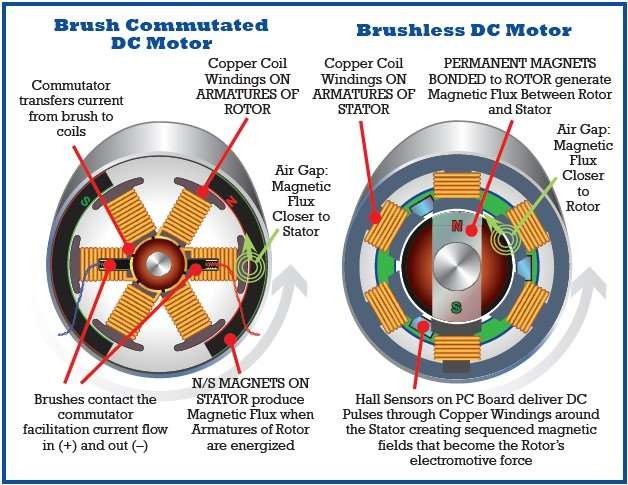
\includegraphics[width=0.5\textwidth]{BLDCBrushedComparison.jpg}
    \caption{Confronto Morfologico Tra Motore DC Con Spazzole (A Sinistra) E Motore BLDC (A Destra)}
\end{figure}
Come mostrato in figura, l'assenza degli avvolgimenti in rame e del collettore a lamelle sul rotore consente di ridurne sensibilmente le dimensioni radiali e la massa complessiva.\\
Ciò comporta una drastica riduzione del \textbf{Momento D'Inerzia $J_m$}, permettendo al servomotore di raggiungere accelerazioni angolari molto elevate ($> 10^4\,\si{\radian\per\second\squared}$), requisito fondamentale nei cicli operativi di \textit{pick-and-place} ad alta cadenza.

\subsubsection{Commutazione Elettronica E Trasduttori Di Posizione}
Il compito principale del sistema di commutazione elettronica è quello di sostituire l'azione del sistema collettore-spazzole. Poiché l'assenza del collettore meccanico elimina l'accoppiamento cinematico diretto tra la posizione geometrica dell'albero e l'alimentazione delle bobine, il controllore elettronico deve rilevare istante per istante la \textbf{posizione angolare del rotore} $\theta_m$.\\
Grazie a questa misura, l'unità di controllo può alimentare la corretta coppia di fasi statoriche al momento opportuno, mantenendo il vettore del campo magnetico di statore sempre in quadratura (ovvero sfasato di $90^\circ$ elettrici) rispetto al flusso magnetico del rotore, in modo da massimizzare la coppia motrice erogata e mantenerne costante il verso.

A seconda della precisione richiesta dal controllo, i trasduttori di posizione impiegati si dividono in tre categorie:
\begin{itemize}
    \item \textbf{Sensori A Effetto Hall Digitali:} Sono costituiti da tre elementi a semiconduttore solidali allo statore, disposti lungo la circonferenza e reciprocamente sfasati di $120^\circ$ (oppure $60^\circ$) elettrici. Al transito dei poli magnetici del rotore, ciascun sensore commuta la propria uscita tra i livelli logici $0$ e $1$. La combinazione binaria delle tre uscite permette di individuare $6$ settori angolari di $60^\circ$ elettrici ciascuno, fornendo la risoluzione discreta necessaria per realizzare la \textbf{commutazione a sei stati} (\textit{six-step trapezoidal commutation}).

    \item \textbf{Encoder Ottici O Magnetici:} Sono trasduttori digitali ad alta risoluzione calettati direttamente sull'albero del motore. Gli \textit{encoder incrementali} (dotati di due canali in quadratura A, B e di una tacca di riferimento di zero Z) offrono risoluzioni che variano da $1000$ a oltre $100\,000$ impulsi per giro. Negli assi dei robot industriali si impiegano prevalentemente \textbf{encoder assoluti monogiro e multigiro} (interfacciati tramite bus seriali sincroni quali EnDat, BiSS o SSI), i quali mantengono l'informazione sulla posizione angolare anche a motore spento, eliminando la necessità di eseguire la procedura di azzeramento (\textit{homing}) all'avvio.

    \item \textbf{Resolver:} Sono trasformatori rotativi di tipo analogico composti da uno statore, provvisto di due avvolgimenti secondari disposti ortogonalmente, e da un rotore eccitato in alta frequenza. Durante la rotazione, il dispositivo restituisce due segnali sinusoidali modulati in ampiezza, proporzionali rispettivamente al seno e al coseno dell'angolo meccanico $\theta_m$. Essendo privi di componenti elettronici delicati a bordo, i resolver risultano immuni a forti disturbi elettromagnetici, temperature elevate ($> 150\,\si{\celsius}$), polveri e vibrazioni meccaniche, trovando largo impiego in fonderie e in ambito aerospaziale.
\end{itemize}

\subsubsection{Vantaggi E Svantaggi Operativi}
Rispetto ai motori DC tradizionali con spazzole, l'architettura costruttiva dei servomotori BLDC offre i seguenti \textbf{vantaggi}:
\begin{enumerate}
    \item \textbf{Efficienza Energetica Superiore:} L'assenza di contatti meccanici striscianti annulla le perdite per attrito radiale e le cadute di tensione elettriche localizzate all'interfaccia spazzola-lamella.
    \item \textbf{Vita Operativa E Ridotta Manutenzione (MTBF Elevato):} L'eliminazione dell'usura meccanica delle spazzole e dell'erosione elettrica del collettore limita il degrado della macchina alla sola durata meccanica dei cuscinetti volventi (generalmente superiore a $20\,000 \div 40\,000$ ore di servizio).
    \item \textbf{Assenza Di Scintillio:} La commutazione statica tramite semiconduttori impedisce l'innesco di archi voltaici, consentendo l'impiego del motore in camere bianche (nessuna emissione di polvere di grafite nell'ambiente) o in atmosfere potenzialmente esplosive e infiammabili.
    \item \textbf{Elevate Velocità Di Rotazione:} L'eliminazione dei limiti meccanici legati alla forza centrifuga agente sulle lamelle del collettore permette di raggiungere velocità di rotazione comprese tra $10\,000$ e oltre $50\,000\,\si{rpm}$.
    \item \textbf{Eccellente Dinamica Di Risposta:} L'elevato rapporto tra coppia motrice erogabile e momento d'inerzia rotorico ($\tau_m / J_m$) assicura un'elevata prontezza di risposta durante i transitori rapidi.
\end{enumerate}

Di contro, l'adozione di questa tecnologia comporta alcuni \textbf{svantaggi}:
\begin{enumerate}
    \item \textbf{Costo Economico Dell'Hardware:} L'impiego di magneti permanenti sinterizzati in terre rare ad alto prodotto d'energia $(BH)_{\max}$ incide sensibilmente sul costo di fabbricazione del motore.
    \item \textbf{Complessità Dell'Elettronica Di Pilotaggio:} Il motore non può essere collegato direttamente a una sorgente in corrente continua, ma richiede obbligatoriamente un azionamento elettronico dedicato, provvisto di microcontrollore o DSP, sensori di corrente, stadi di isolamento galvanico/ottico e un inverter trifase a semiconduttori di potenza.
\end{enumerate}
\newpage

\subsection{Il Motore BLDC Trifase E Il Circuito Di Pilotaggio Ad Inverter}

\subsubsection{Configurazione Trifase E Relazioni Elettromeccaniche}
I servomotori BLDC impiegati in ambito robotico adottano tipicamente una configurazione di tipo \textbf{trifase sincrono}, in cui lo statore ospita tre avvolgimenti indipendenti sfasati geometricamente nello spazio di $120^\circ$ elettrici.\\
Indicando con $p$ il \textbf{numero di coppie polari} del rotore, un giro meccanico completo ($360^\circ$ meccanici) corrisponde a $p$ cicli completi del campo magnetico ($p \cdot 360^\circ$ elettrici). Di conseguenza, il legame tra l'angolo meccanico del rotore $\theta_m$ e l'angolo elettrico $\theta_e$ è espresso dalla relazione:
\[
    \theta_e = p \cdot \theta_m
\]
Derivando rispetto al tempo, si ottiene che la pulsazione elettrica $\omega_e$ delle correnti statoriche è direttamente proporzionale alla velocità angolare meccanica $\omega_m$ dell'albero:
\[
    \omega_e = p \cdot \omega_m
\]

\subsubsection{Architettura Dell'Inverter A Ponte Trifase}
Il controllo dell'ampiezza, della frequenza e del verso delle correnti che attraversano gli avvolgimenti di fase è affidato a un convertitore statico di potenza, denominato \textbf{inverter trifase a ponte intero}.

\begin{figure}[H]
    \centering
    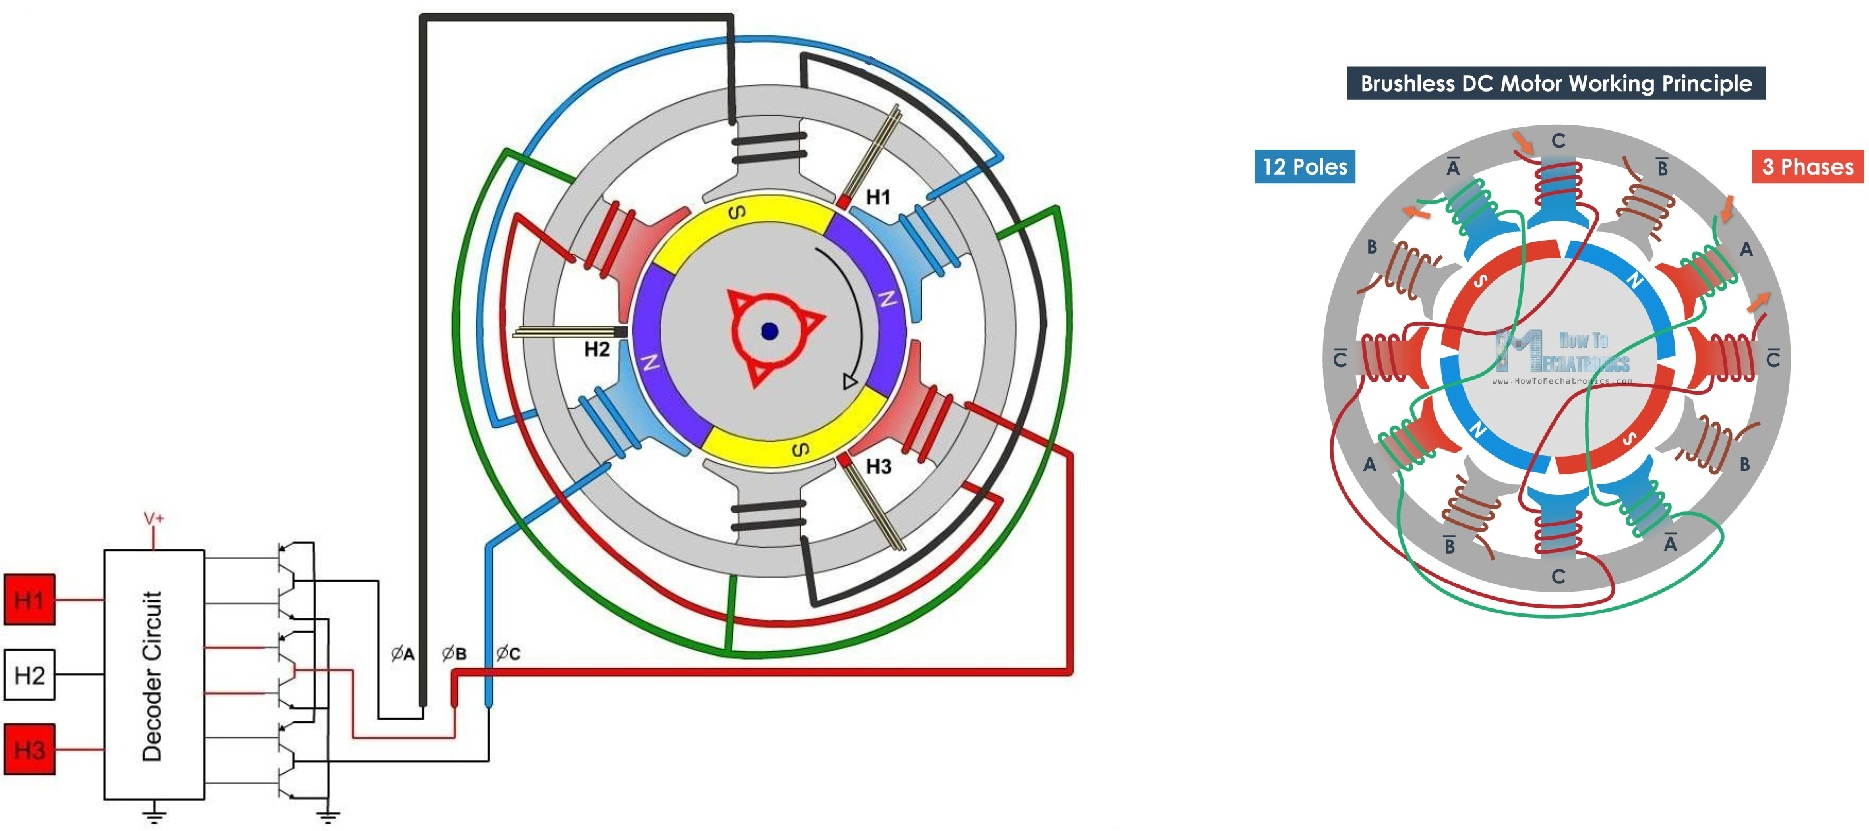
\includegraphics[width=0.8\textwidth]{BLDCHBridgeDriver.jpg}
    \caption{Schema Elettrico Di Un Inverter A Ponte Trifase A 6 Interruttori (MOSFET O IGBT) Per Il Pilotaggio Di Un Servomotore BLDC Con Avvolgimenti Collegati A Stella E Centro-Stella Non Accessibile.}
    \label{fig:bldc_inverter}
\end{figure}

Come illustrato in figura, il circuito viene alimentato da un bus in tensione continua $V_{DC}$, ottenuto mediante il raddrizzamento e il successivo livellamento capacitivo della tensione alternata di rete. La struttura del ponte si compone di tre rami in parallelo (\textit{legs}), ciascuno associato a una delle tre fasi statoriche (U, V, W):
\begin{itemize}
    \item \textbf{Ramo Della Fase U:} Costituito dall'interruttore superiore $Q_1$ (\textit{High-Side}), collegato al polo positivo $+V_{DC}$, e dall'interruttore inferiore $Q_2$ (\textit{Low-Side}), collegato al riferimento di massa.
    \item \textbf{Ramo Della Fase V:} Costituito dall'interruttore superiore $Q_3$ (\textit{High-Side}) e dall'interruttore inferiore $Q_4$ (\textit{Low-Side}).
    \item \textbf{Ramo Della Fase W:} Costituito dall'interruttore superiore $Q_5$ (\textit{High-Side}) e dall'interruttore inferiore $Q_6$ (\textit{Low-Side}).
\end{itemize}
Gli interruttori elettronici vengono realizzati mediante transistor MOSFET di potenza per tensioni di bus inferiori a $100\,\si{\volt}$, oppure tramite IGBT per livelli di tensione e potenza superiori. Ciascun transistor è affiancato da un diodo collegato in antiparallelo, detto \textbf{diodo di ricircolo} (\textit{freewheeling diode}), che offre una via di continuità alle correnti induttive di fase durante le fasi di interdizione degli interruttori.\\
Inoltre, per evitare che entrambi i transistor appartenenti allo stesso ramo conducano simultaneamente generando un cortocircuito netto sul bus di alimentazione (fenomeno di \textit{shoot-through}), i segnali di comando per l'apertura e la chiusura degli interruttori complementari vengono separati da un breve intervallo di sicurezza, denominato \textbf{tempo morto} (\textit{dead-time}).
\newpage

\subsubsection{Logica Di Commutazione A Sei Passi (Six-Step Control)}
Nella tecnica di pilotaggio trapezoidale a sei passi (\textit{Six-Step Control}), il periodo elettrico completo di $360^\circ$ viene suddiviso in sei settori angolari discreti, ciascuno di ampiezza pari a $60^\circ$ elettrici.\\
All'interno di ogni singolo settore, solamente due delle tre fasi statoriche vengono connesse attivamente al bus di alimentazione: un interruttore superiore (\textit{High-Side}) viene chiuso per iniettare corrente dal terminale $+V_{DC}$ verso un primo avvolgimento di fase, mentre un interruttore inferiore (\textit{Low-Side}) appartenente a un altro ramo viene chiuso per permettere il ritorno della corrente verso massa attraverso un secondo avvolgimento. Contemporaneamente, la terza fase non viene alimentata e rimane elettricamente flottante (\textit{floating}).

Durante la rotazione dell'albero, i tre sensori a effetto Hall rilevano il passaggio dei poli rotorici da un settore al successivo. La decodifica logica della parola binaria a 3 bit generata dai sensori ($100_2 \to 110_2 \to 010_2 \dots$) permette al microcontrollore di comandare l'accensione sincronizzata dei gate dei transistor secondo la seguente sequenza ciclica:
\begin{align*}
    \text{Settore 1: } & Q_1 \text{ ON (Fase U a } +V_{DC}\text{)}, & Q_4 \text{ ON (Fase V a massa)}, \quad & \text{Fase W scollegata} \\
    \text{Settore 2: } & Q_1 \text{ ON (Fase U a } +V_{DC}\text{)}, & Q_6 \text{ ON (Fase W a massa)}, \quad & \text{Fase V scollegata} \\
    \text{Settore 3: } & Q_3 \text{ ON (Fase V a } +V_{DC}\text{)}, & Q_6 \text{ ON (Fase W a massa)}, \quad & \text{Fase U scollegata} \\
    \text{Settore 4: } & Q_3 \text{ ON (Fase V a } +V_{DC}\text{)}, & Q_2 \text{ ON (Fase U a massa)}, \quad & \text{Fase W scollegata} \\
    \text{Settore 5: } & Q_5 \text{ ON (Fase W a } +V_{DC}\text{)}, & Q_2 \text{ ON (Fase U a massa)}, \quad & \text{Fase V scollegata} \\
    \text{Settore 6: } & Q_5 \text{ ON (Fase W a } +V_{DC}\text{)}, & Q_4 \text{ ON (Fase V a massa)}, \quad & \text{Fase U scollegata}
\end{align*}

L'esecuzione continua di questa sequenza genera all'interno dello statore un campo magnetico che ruota nello spazio a passi discreti di $60^\circ$ elettrici. Poiché la commutazione è vincolata alla posizione istantanea del rotore, i poli magnetici rotorici vengono costantemente attratti dal campo statorico, trascinando l'albero in rotazione sincrona.\\
Infine, per regolare la velocità e la coppia del motore, agli interruttori attivi (tipicamente gli \textit{High-Side}) non viene applicato un comando di chiusura fisso, bensì un segnale modulato ad alta frequenza ($10 \div 20\,\si{\kilo\hertz}$) tramite tecnica \textbf{PWM} (\textit{Pulse Width Modulation}). Variando il \textit{duty-cycle} della modulazione PWM si controlla la tensione media applicata agli avvolgimenti e, di conseguenza, l'intensità della corrente di fase $I_a$, permettendo di governare con precisione la coppia motrice erogata e il profilo cinematico del giunto robotico.

\section{La Trasmissione Meccanica Nei Sistemi Robotici}

Nell'architettura di un robot industriale, la \textbf{trasmissione meccanica} collega l'albero d'uscita dell'attuatore (tipicamente un servomotore rotativo) al rispettivo giunto (\textit{joint}) del braccio rigido (\textit{link}). L'azionamento diretto (\textit{direct-drive}) è limitato ad applicazioni specifiche a causa della ridotta densità di coppia dei motori elettrici e del loro riscaldamento per effetto Joule a basse velocità.

L'interposizione della trasmissione risponde a tre esigenze:

\begin{enumerate}
    \item \textbf{Adattamento Meccanico E Moltiplicazione Della Coppia (\textit{Impedance Matching})}: I servomotori elettrici (sia \textit{brushless} sia in corrente continua) erogano la massima densità di potenza ad alte velocità ($2\,000 \div 6\,000\,\si{rpm}$, ovvero $\omega_m \approx 200 \div 600\,\si{\radian\per\second}$) con coppie nominali continuative contenute (da frazioni a pochi $\si{\newton\meter}$). I giunti di un manipolatore seriale richiedono invece basse velocità ($30 \div 60\,\si{rpm}$, ovvero $\omega_L \approx 3 \div 6\,\si{\radian\per\second}$) ed elevate coppie statiche e dinamiche (da decine a migliaia di $\si{\newton\meter}$) per contrastare carichi gravitazionali $\bm{g}(\bm{q})$, forze centrifughe e di Coriolis $\bm{C}(\bm{q},\dot{\bm{q}})\dot{\bm{q}}$, e accelerare le inerzie $\bm{M}(\bm{q})\ddot{\bm{q}}$. Il riduttore meccanico riduce la velocità angolare amplificando contestualmente la coppia erogata in base al \textbf{rapporto di riduzione}. Inoltre, l'inerzia del carico $J_L$ riflessa all'asse motore scala quadraticamente ($J_L' = \tau^2 J_L$), favorendo stabilità e controllabilità.

    \item \textbf{Conversione Della Morfologia Del Moto}: Converte il moto puramente rotatorio dell'attuatore nello spostamento traslatorio richiesto da giunti prismatici (carrelli lineari o assi verticali di robot cartesiani).

    \item \textbf{Ottimizzazione Della Distribuzione Delle Masse E Delle Prestazioni Dinamiche}: In catene seriali a sbalzo, montare ciascun motore sul rispettivo giunto appesantisce i membri a monte, accrescendone momento flettente e coppie necessarie. Trasmissioni remote (cinghie dentate, alberi coassiali o catene) consentono di collocare i motori in prossimità del basamento, riducendo le inerzie mobili a vantaggio delle accelerazioni, del tempo di ciclo e dell'accuratezza di inseguimento.
\end{enumerate}

\subsection{Panoramica Delle Principali Tecnologie Di Trasmissione}

Le trasmissioni impiegate nella robotica industriale differiscono per accoppiamento, rendimento, rigidezza elastica e accuratezza di posizionamento:

\noindent
\begin{minipage}[t]{0.48\textwidth}
    \textbf{Ingranaggi Dentati Cilindrici e Conici}
    \par\vspace{0.2cm}
    Trasmettono moto tra assi adiacenti, variando rapporto di velocità, coppia, senso di rotazione e orientamento spaziale (da paralleli a concorrenti). Presentano rigidezza torsionale finita sotto carichi ciclici elevati e \textbf{gioco angolare} (\textit{backlash}), sorgente di zona morta (\textit{deadband}) critica nelle inversioni di moto retroazionate.
    \begin{figure}[H]
        \centering
        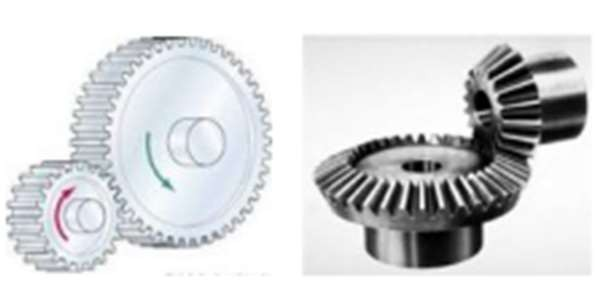
\includegraphics[width=0.6\linewidth]{IngranaggiDentati.jpg}
        \caption{Coppia Di Ruote Dentate Cilindriche Ad Assi Paralleli.}
    \end{figure}
\end{minipage}
\hfill
\begin{minipage}[t]{0.48\textwidth}
    \textbf{Viti A Ricircolo Di Sfere E Viti Senza Fine}
    \par\vspace{0.2cm}
    Convertono il moto rotativo in traslatorio nei giunti prismatici. Le viti a ricircolo di sfere sostituiscono il contatto radente delle madreviti convenzionali con l'attrito volvente, assicurando rendimenti superiori al $90\%$, elevata rigidezza assiale e annullamento del gioco mediante precarico. Le viti a strisciamento presentano invece rendimenti inferiori e usura progressiva.
    \begin{figure}[H]
        \centering
        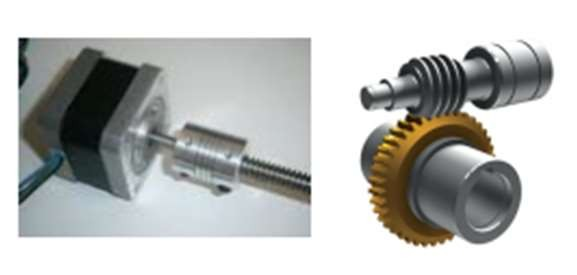
\includegraphics[width=0.6\linewidth]{RicircoloViti.jpg}
        \caption{Chiocciola A Ricircolo Di Sfere Per Attuazione Lineare.}
        \label{fig:ricircolo_viti}
    \end{figure}
\end{minipage}

\newpage

\noindent
\begin{minipage}[t]{0.48\textwidth}
    \textbf{Cinghie Dentate E Catene Di Trasmissione}
    \par\vspace{0.2cm}
    Trasmettono potenza tra assi paralleli distanziati, svincolando la posizione del motore da quella del giunto. Le cinghie sincrone dentate in elastomero con armature in acciaio garantiscono silenziosità, assenza di lubrificazione e isolamento elettrico, ma introducono cedevolezza elastica longitudinale che abbassa le risonanze strutturali. Le catene metalliche sostengono carichi superiori, ma la massa rilevante induce forze d'inerzia e vibrazioni ad alti regimi.
    \begin{figure}[H]
        \centering
        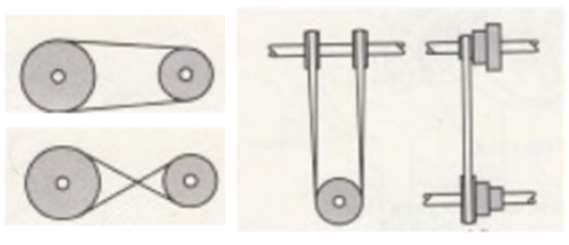
\includegraphics[width=0.6\linewidth]{CinghieCatene.jpg}
        \caption{Trasmissione Flessibile A Cinghia Sincrona Dentata.}
    \end{figure}
\end{minipage}
\hfill
\begin{minipage}[t]{0.48\textwidth}
    \textbf{Riduttori Armonici (\textit{Harmonic Drives})}
    \par\vspace{0.2cm}
    Impiegati nei giunti di robot antropomorfi, cobot e manipolatori di precisione. Sfruttando la deformazione elastica ciclica di una boccola metallica flessibile, ottengono elevati rapporti di riduzione (da $30:1$ a oltre $160:1$) in un singolo stadio coassiale compatto, privo di gioco angolare (\textit{zero-backlash}). Richiedono tuttavia compensazione della cedevolezza torsionale distribuita a livello di controllo.
    \begin{figure}[H]
        \centering
        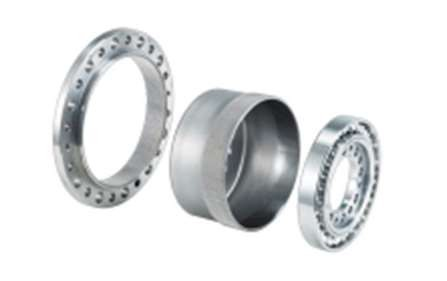
\includegraphics[width=0.6\linewidth]{HarmonicDrives.jpg}
        \caption{Gruppo Riduttore Armonico Coassiale Integrato.}
    \end{figure}
\end{minipage}

\newpage

\section{Teoria Meccanica Dei Rotismi E Delle Ruote Dentate}

Un \textbf{ingranaggio} trasmette moto e potenza mediante contatto di forma tra denti, senza slittamento macroscopico. Una sequenza di due o più ruote dentate vincolate costituisce un \textbf{rotismo} (o treno di ingranaggi).

\subsection{Accoppiamento Cinematica E Geometria Degli Assi}

La conformazione delle ruote dipende dalla disposizione reciproca degli assi di ingresso e uscita:

\begin{enumerate}
    \item \textbf{Assi Paralleli}: Si impiegano \textbf{ingranaggi cilindrici}, le cui superfici primitive sono cilindri retti a rotolamento puro. Le dentature possono essere diritte (semplici, prive di spinte assiali, ma rumorose ad alta velocità) o elicoidali (ingranamento progressivo, maggiore capacità di carico e silenziosità, con insorgenza di una spinta assiale che richiede supporti reggispinta).
    \item \textbf{Assi Concorrenti (o Incidenti)}: Quando gli assi sono complanari e incidenti (tipicamente a $90^\circ$, come nei polsi robotici), si adottano \textbf{ingranaggi conici}. Le superfici primitive sono tronchi di cono con vertice coincidente nel punto d'intersezione degli assi. I denti possono essere diritti o spiroidali (es. profilo Gleason).
    \item \textbf{Assi Sghembi}: In assenza di complanarità e intersezione, la trasmissione avviene mediante ruote elicoidali per assi sghembi, ingranaggi ipoidi o coppie \textbf{vite senza fine e ruota elicoidale}. Queste ultime offrono rapporti elevati in ingombri ridotti e consentono l'\textit{irreversibilità meccanica} (trasmissione possibile unicamente dalla vite alla ruota), garantendo l'arresto statico del carico a motore disalimentato.
\end{enumerate}

Le figure seguenti illustrano le geometrie e i diagrammi funzionali corrispondenti.

\begin{figure}[H]
    \centering
    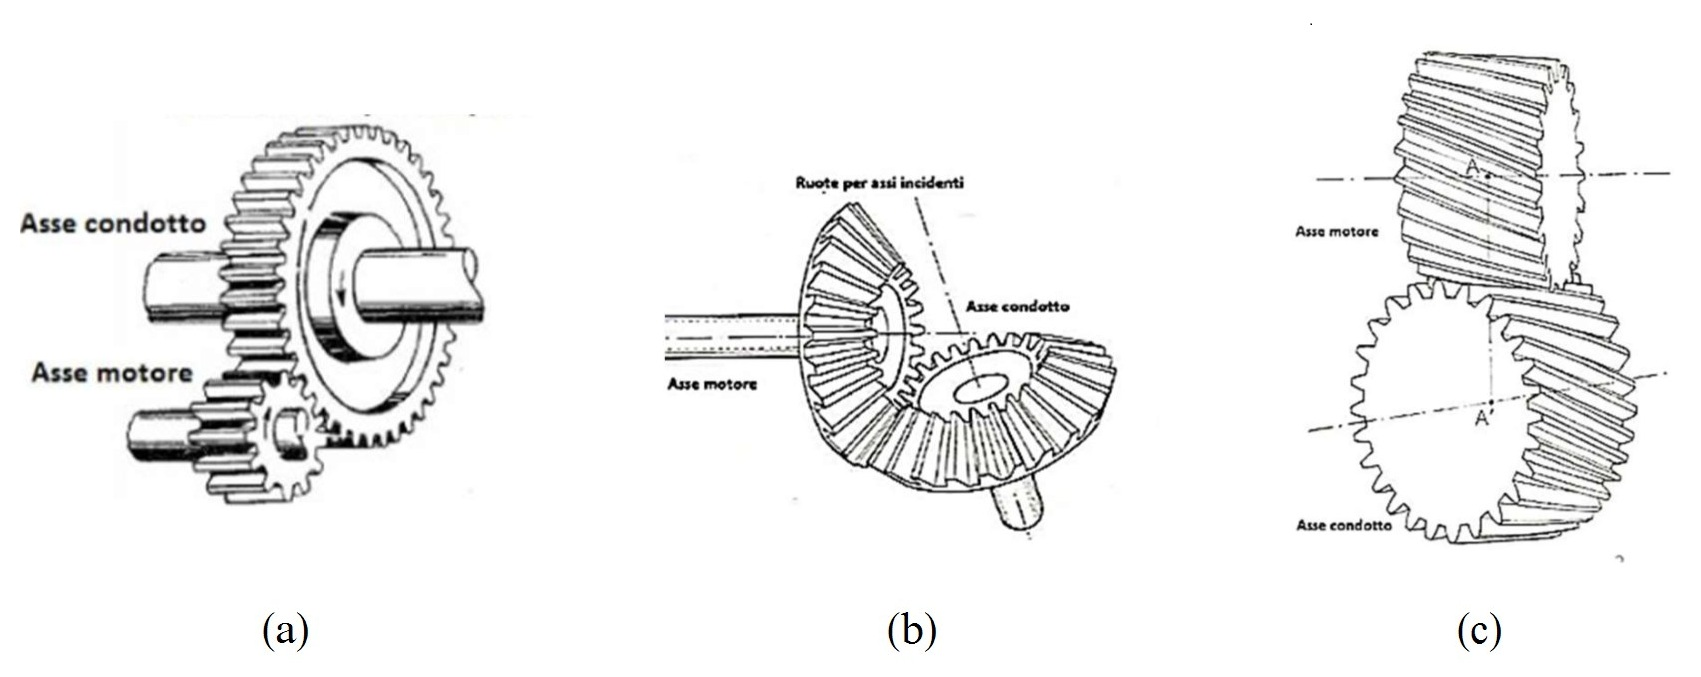
\includegraphics[width=0.6\linewidth]{Ingranaggi.jpeg}
    \caption{Classificazione Geometrica Dei Componenti Dentati: (a) Ingranaggio Cilindrico A Denti Diritti Per Assi Paralleli, (b) Ingranaggio Conico A Denti Diritti Per Assi Concorrenti, (c) Ingranaggi Elicoidali E Vite Senza Fine Per Assi Sghembi.}
\end{figure}

\begin{figure}[H]
    \centering
    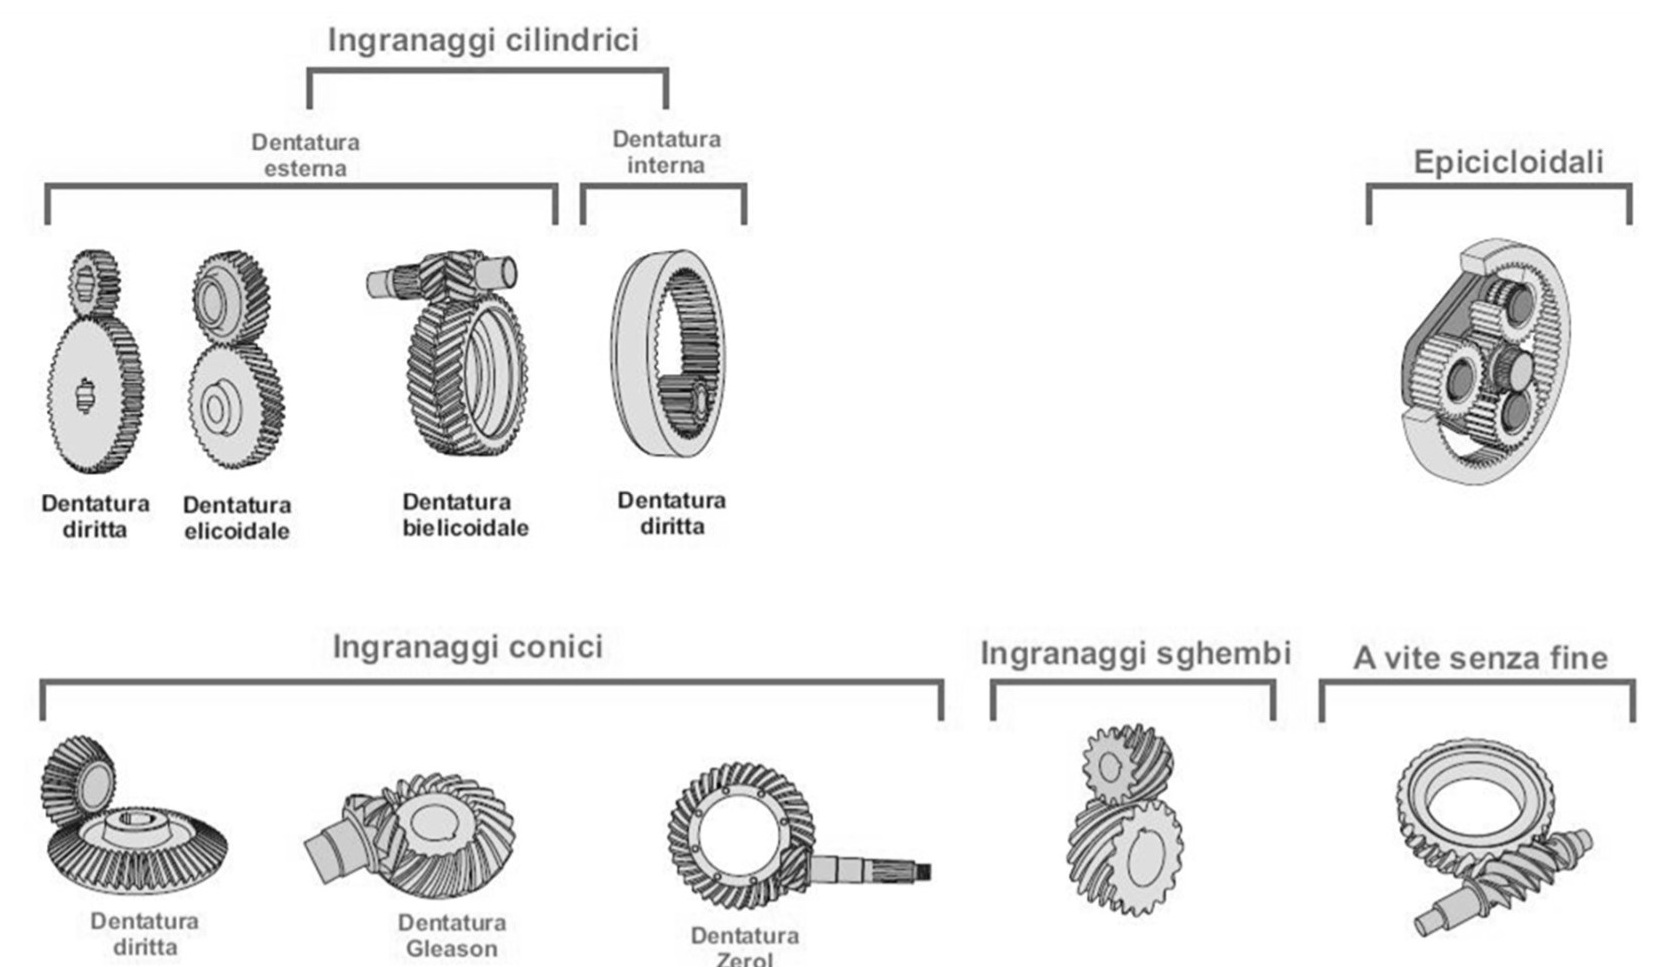
\includegraphics[width=0.6\linewidth]{SchemaIngranaggi.jpeg}
    \caption{Schematizzazione Funzionale E Tracciato Delle Forze Di Contatto Nelle Principali Geometrie Di Ruote Dentate.}
\end{figure}

\newpage

\subsection{Classificazione Meccanica Dei Rotismi}

In base alla cinematica degli assi e alla struttura dell'alberaggio, i rotismi si classificano in:

\begin{itemize}
    \item \textbf{Rotismo Piano:} Assi reciprocamente paralleli; le traiettorie dei punti giacciono su piani ortogonali agli assi.
    \item \textbf{Rotismo Sferico:} Assi concorrenti in un punto fisso; le traiettorie descrivono archi su superfici sferiche concentriche.
    \item \textbf{Rotismo Ordinario:} Assi di rotazione tutti \textbf{fissi rispetto al telaio}. Si articola in:
    \begin{itemize}
        \item \textbf{Rotismo Semplice}: Ciascun albero porta un'unica ruota dentata.
        \item \textbf{Rotismo Composto}: Almeno un albero intermedio porta calettate due o più ruote dentate solidali, aventi la medesima velocità angolare.
    \end{itemize}
    \item \textbf{Rotismo Epicicloidale (o Planetario):} Almeno un asse di rotazione (ruota satellite o pianeta) \textbf{è mobile nello spazio}, muovendosi lungo una traiettoria circolare guidata da un braccio portasatelliti imperniato sull'asse principale.
\end{itemize}

\begin{figure}[H]
    \centering
    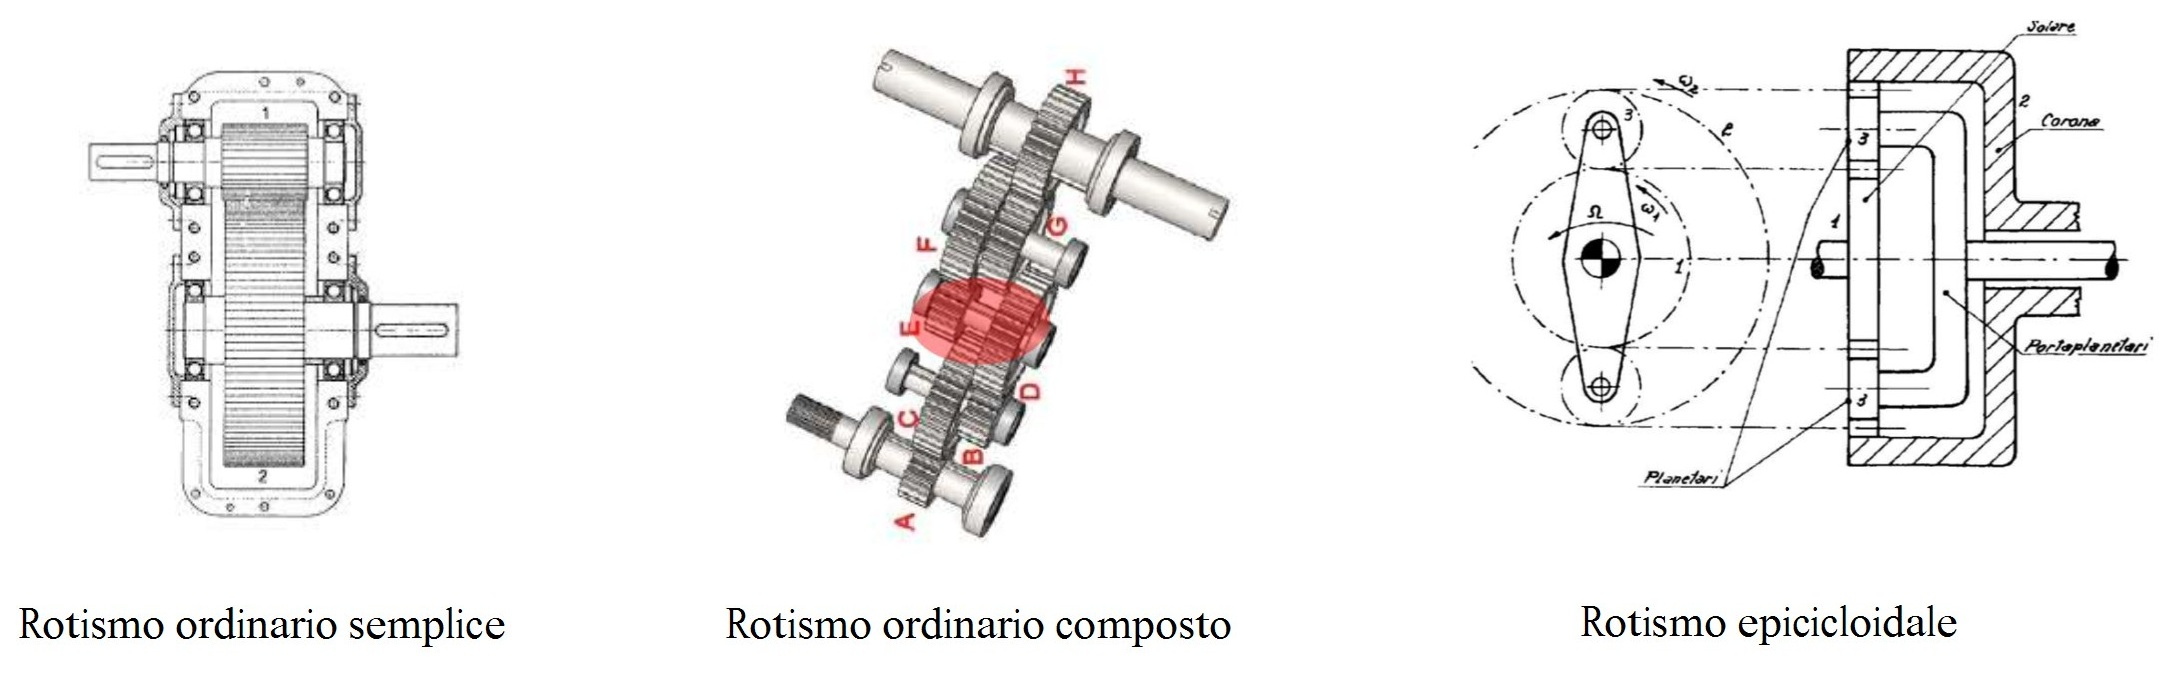
\includegraphics[width=0.8\linewidth]{EsempiRotismo.jpeg}
    \caption{Tipologie Strutturali Di Rotismi: Confronto Tra Rotismi Ordinari A Cascata (Semplici E Composti) E Rotismi Epicicloidali Ad Assi Planetari Mobili.}
\end{figure}

\subsection{Rapporto Di Trasmissione: Analisi Cinematica E Statica}

Il \textbf{rapporto di trasmissione} (o di velocità) $\tau$ è il rapporto algebrico tra la velocità angolare d'uscita ($\omega_{\text{out}}$) e quella d'ingresso ($\omega_{\text{in}}$):
\[
    \tau = \frac{\omega_{\text{out}}}{\omega_{\text{in}}}
    \label{eq:def_tau}
\]
Il rapporto di riduzione $i$ è definito come il reciproco $i = 1/\tau = \omega_{\text{in}}/\omega_{\text{out}}$. Nel seguito si adotta la convenzione $\tau = \omega_{\text{out}}/\omega_{\text{in}}$, per cui un riduttore di velocità soddisfa $|\tau| < 1$.

\subsubsection{Ingranaggio Singolo Elementare Ad Assi Paralleli}
Date due ruote $a$ e $b$ montate su perni fissi paralleli, con dentature $z_a, z_b$ e raggi primitivi $r_a, r_b$, l'ingranamento richiede il medesimo \textbf{modulo normale} $m$ (in $\si{\milli\meter}$), definito come rapporto tra diametro primitivo $d = 2r$ e numero di denti $z$:
\[
    m = \frac{d_a}{z_a} = \frac{d_b}{z_b} \implies r_a = \frac{m z_a}{2}, \quad r_b = \frac{m z_b}{2}
\]
Il passo primitivo è $p = \pi m$. Poiché nel punto di contatto primitivo $C$ vi è rotolamento puro senza strisciamento tangenziale, le velocità periferiche coincidono:
\[
    v_c = \omega_a r_a = -\omega_b r_b
\]
dove il segno negativo indica che per dentature esterne le rotazioni hanno versi opposti.\\
Sostituendo $r_a$ e $r_b$
\[
    \tau_{a,b} = \frac{\omega_b}{\omega_a} = -\frac{r_a}{r_b} = -\frac{z_a}{z_b}
    \label{eq:rapporto_singolo}
\]
In presenza di dentatura interna, i membri ruotano concordemente: $\tau = +z_a/z_b$.
\newpage

\subsubsection{Rotismo Composto A Cascata}
Poiché rapporti di riduzione elevati ($|\tau| \ll 1$) a singolo stadio richiederebbero ingombri radiali inaccettabili ($z_b = z_a / |\tau|$), si ricorre al \textbf{rotismo composto}, ripartendo la riduzione su più stadi in serie. Per una catena ordinaria di $k$ coppie in cascata tra l'albero movente $1$ e il cedente $n$, il rapporto di trasmissione globale $\tau$ è il prodotto dei rapporti delle singole coppie:
\[
    \tau = \frac{\omega_n}{\omega_1} = \prod_{i=1}^{k} \tau_{i} = (-1)^{p_{\text{est}}} \frac{\prod z_{\text{motrici}}}{\prod z_{\text{condotte}}}
    \label{eq:formula_generale_rotismo}
\]
dove $p_{\text{est}}$ indica il numero di contatti a dentatura esterna lungo la catena, ciascuno determinante un'inversione del verso di rotazione.

\subsubsection*{Esempio Analitico Svolto: Rotismo Composto A Due Stadi}

Si consideri il rotismo in figura: la ruota motrice $a$ aziona la ruota $b$; solidale e coassiale a $b$ è montata la ruota $c$ ($\omega_c \equiv \omega_b$); la ruota $c$ aziona infine la ruota d'uscita $d$.

\noindent
\begin{minipage}[c]{0.48\textwidth}
    \begin{figure}[H]
        \centering
        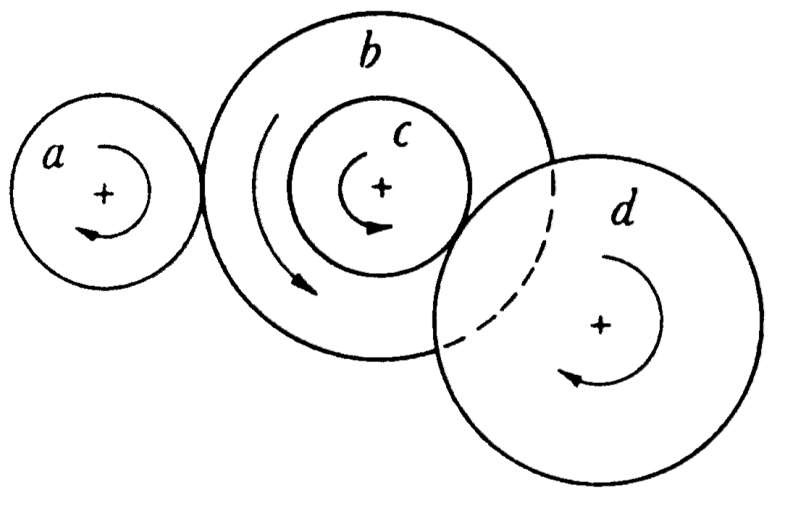
\includegraphics[width=0.7\linewidth]{EsempioAnalisi.jpg}
        \caption{Schema Cinematico Del Rotismo Composto A 4 Ruote Dentate ($a, b, c, d$).}
    \end{figure}
\end{minipage}
\hfill
\begin{minipage}[c]{0.48\textwidth}
    I rapporti di trasmissione per le due coppie ad assi fissi valgono:
    \begin{align}
        \tau_{a,b} &= \frac{\omega_b}{\omega_a} = -\frac{z_a}{z_b}\\
        \tau_{c,d} &= \frac{\omega_d}{\omega_c} = -\frac{z_c}{z_d}
    \end{align}
\end{minipage}

\vspace{0.3cm}
\noindent
Essendo $\omega_c = \omega_b$, il rapporto globale $\tau_{a,d}$ tra uscita $d$ e ingresso $a$ si espande mediante la regola della catena:
\[
    \tau_{a,d} = \frac{\omega_d}{\omega_a} = \frac{\omega_d}{\omega_c} \cdot \frac{\omega_b}{\omega_a} = \tau_{c,d} \cdot \tau_{a,b}
\]
Sostituendo le equazioni di $\tau_{a,b}$ e di $\tau_{c,d}$
\[
    \tau_{a,d} = \left(-\frac{z_c}{z_d}\right) \cdot \left(-\frac{z_a}{z_b}\right) = +\frac{z_a z_c}{z_b z_d}
\]
La presenza di due contatti esterni consecutivi rende positivo il rapporto ($\tau_{a,d} > 0$): l'uscita $d$ ruota nello stesso verso dell'ingresso $a$.

\subsubsection{Bilancio Di Potenza Ed Equilibrio Delle Coppie}
In regime stazionario ($\dot{\omega} = 0$) e in condizioni ideali a \textbf{rendimento unitario} ($\eta = 1$), in assenza di perdite per attrito di strisciamento e nei supporti, la conservazione dell'energia impone $P_{\text{in}} = P_{\text{out}}$:
\[
    P_{\text{in}} = P_{\text{out}} \implies C_m \cdot \omega_m = C_r \cdot \omega_r
    \label{eq:conservazione_potenza}
\]
Dove:
\begin{itemize}
    \item $C_m$ è la coppia motrice all'albero d'ingresso [$\si{\newton\meter}$];
    \item $\omega_m = \omega_{\text{in}}$ è la velocità angolare motrice [$\si{\radian\per\second}$];
    \item $C_r$ è la coppia utile al carico all'albero d'uscita [$\si{\newton\meter}$];
    \item $\omega_r = \omega_{\text{out}}$ è la velocità angolare resistente d'uscita [$\si{\radian\per\second}$].
\end{itemize}

Sostituendo $\tau = \omega_r / \omega_m$ nell'equazione precedente, si ottiene il bilancio delle coppie:
\[
    \frac{C_r}{C_m} = \frac{\omega_m}{\omega_r} = \frac{1}{\tau} \implies C_r = \frac{1}{\tau} \cdot C_m
\]
Quest'equazione mostra che un riduttore di velocità ($|\tau| < 1$) moltiplica idealmente la coppia motrice di un fattore $1/|\tau|$.

\paragraph{Caso Reale Con Rendimento Meccanico e Dinamica delle Masse}
Nel caso reale, attriti di contatto, sbattimento del lubrificante (\textit{churning losses}) e rotolamento nei supporti determinano un \textbf{rendimento meccanico} $\eta < 1$ ($\eta \approx 0.95 \div 0.98$ per singolo stadio cilindrico di precisione):
\[
    P_{\text{out}} = \eta \cdot P_{\text{in}} \implies C_r \omega_r = \eta \cdot (C_m \omega_m) \implies C_r = \eta \cdot \frac{C_m}{\tau}
\]
Durante i transitori di accelerazione ($\dot{\omega} \neq 0$), l'equazione del moto all'albero motore, comprensiva dell'inerzia del rotore $J_m$, del riduttore $J_{\text{rid}}$ e del link $J_L$, assume la forma:
\[
    C_m - \tau \cdot \frac{C_{\text{ext}}}{\eta} = \left( J_m + J_{\text{rid}} + \frac{\tau^2}{\eta} J_L \right) \dot{\omega}_m + \beta_m \omega_m
    \label{eq:dinamica_motore_riduttore}
\]
dove $\beta_m$ è il coefficiente d'attrito viscoso e $C_{\text{ext}}$ la coppia esterna applicata al link. L'inerzia del carico riflessa scala con $\tau^2$: per $\tau = 0.01$ (riduzione $1:100$), $J_L$ riflessa all'asse motore risulta attenuata di un fattore $10^{-4}$, disaccoppiando la dinamica del rotore dalle variazioni di carico.

\subsection{La Ruota Dentata Oziosa}

Nei rotismi ordinari semplici ad assi paralleli, la \textbf{ruota oziosa} (\textit{idler gear}) è una ruota intermedia montata su perno fisso che ingrana simultaneamente con la ruota motrice e con la ruota condotta.

\noindent
\begin{minipage}[c]{0.48\textwidth}
    \begin{figure}[H]
        \centering
        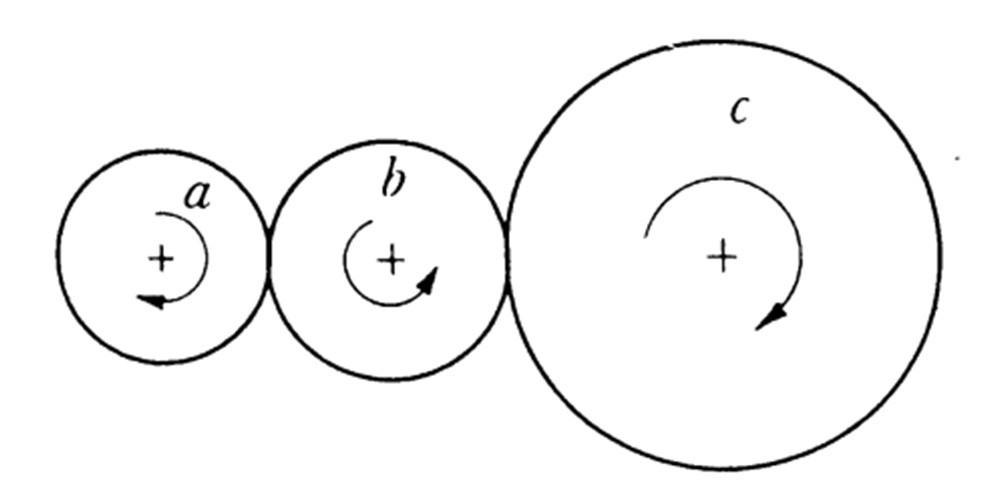
\includegraphics[width=0.7\linewidth]{EsempioRuotaOziosa.jpg}
        \caption{Rotismo Semplice A Tre Ruote Con Ruota Intermedia Oziosa $b$.}
    \end{figure}
\end{minipage}
\hfill
\begin{minipage}[c]{0.48\textwidth}
    Per le coppie adiacenti di Figura~\ref{fig:ruota_oziosa}, con ruota motrice $a$, oziosa $b$ e condotta $c$:
    \[
        \tau_{a,b} = \frac{\omega_b}{\omega_a} = -\frac{z_a}{z_b}
    \]
    \[
        \tau_{b,c} = \frac{\omega_c}{\omega_b} = -\frac{z_b}{z_c}
    \]
\end{minipage}

\vspace{0.3cm}
\noindent
Il rapporto globale tra ruota condotta $c$ e motrice $a$ è:
\[
    \tau_{a,c} = \frac{\omega_c}{\omega_a} = \tau_{b,c} \cdot \tau_{a,b} = \left(-\frac{z_b}{z_c}\right) \cdot \left(-\frac{z_a}{z_b}\right) = +\frac{z_a}{z_c}
    \label{eq:semplificazione_oziosa}
\]
Il parametro $z_b$ si semplifica algebricamente: il rapporto di velocità è indipendente dalle dimensioni della ruota oziosa. La ruota oziosa assolve a due funzioni:
\begin{enumerate}
    \item \textbf{Inversione Del Verso Di Rotazione}: L'accoppiamento diretto $a$-$c$ imporrebbe rotazione contraria ($\tau = -z_a/z_c$), mentre l'inserimento dell'oziosa garantisce rotazione concorde ($\tau > 0$).
    \item \textbf{Superamento Di Distanze Meccaniche}: Collega assi distanziati senza impiegare ruote di raggio primitivo elevato, limitando gli ingombri.
\end{enumerate}

\newpage

\subsection{Caso Particolare: Meccanismo Pignone E Cremagliera}

Il sistema \textbf{pignone e cremagliera} (\textit{rack and pinion}) rappresenta la configurazione limite di una coppia di ruote cilindriche in cui il raggio primitivo di una ruota tende all'infinito ($r_c \to \infty$), degenerando in un'asta dentata rettilinea (\textbf{cremagliera}). Il sistema opera come convertitore bidirezionale tra rotazione e traslazione:
\begin{itemize}
    \item Posto in rotazione il pignone di raggio primitivo $r_p$ alla velocità $\omega_p$ su perno fisso, la cremagliera trasla a velocità:
    \[
        v_c = \omega_p \cdot r_p = \omega_p \cdot \frac{m z_p}{2}
    \]
    \item Imponendo una traslazione alla cremagliera, le forze tangenziali sui denti trascinano in rotazione il pignone.
\end{itemize}

\begin{figure}[H]
    \centering
    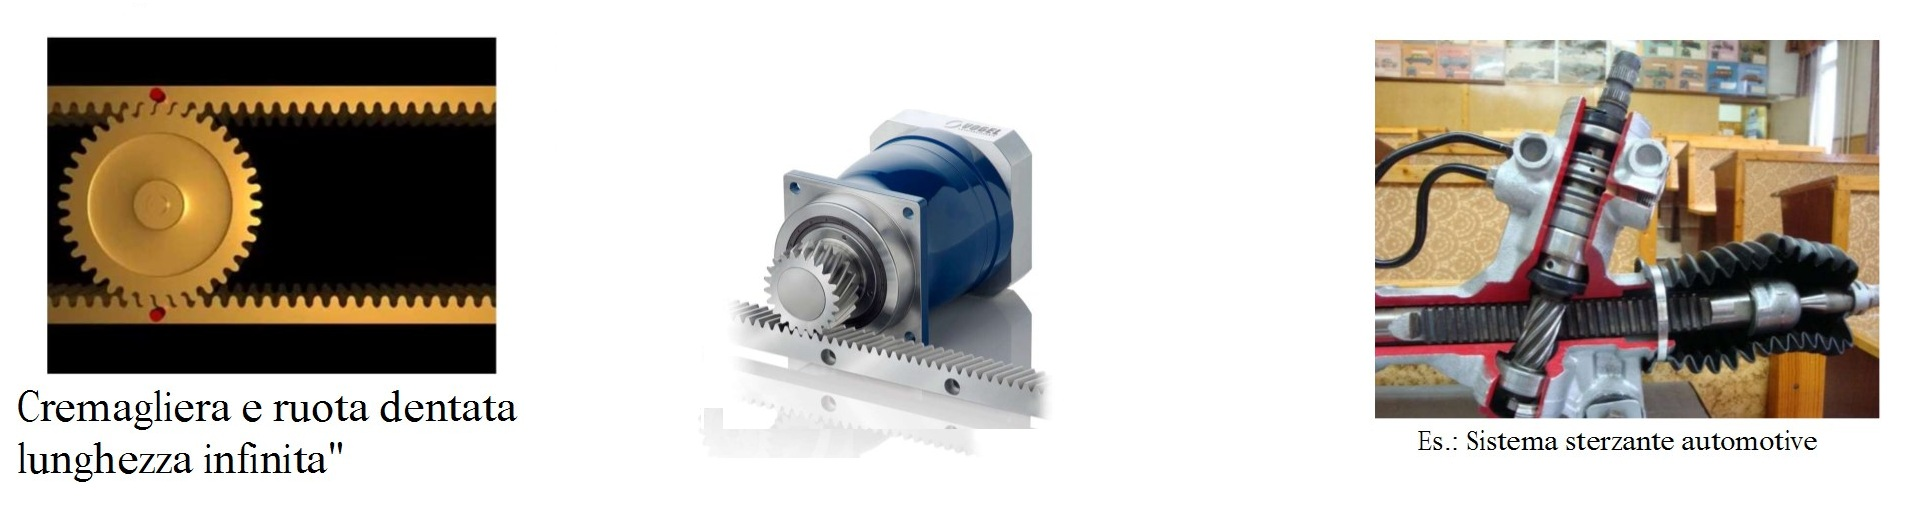
\includegraphics[width=0.75\linewidth]{CremaglieraPignone.jpeg}
    \caption{Cinematica Del Sistema Pignone-Cremagliera: Conversione Tra Velocità Angolare $\omega_p$ E Velocità Traslatoria Uniforme $v_c$.}
\end{figure}
Il meccanismo è impiegato nei gruppi sterzo e nel \textbf{settimo asse di scorrimento} (\textit{runway track}) di robot industriali, ove lunghezze di corsa elevate impediscono l'adozione di viti a ricircolo di sfere a causa dell'inflessione e dell'innesco di velocità critiche flessionali.

\newpage

\section{Rotismi Epicicloidali (O Planetari)}
Un \textbf{rotismo epicicloidale} (o riduttore planetario, \textit{planetary gear}) è una catena cinematica di ruote dentate in cui gli assi di una o più ruote \textbf{orbitano nello spazio} attorno all'asse principale anziché essere fissi rispetto al telaio.

Questa topologia presenta tre vantaggi principali:
\begin{itemize}
    \item \textbf{Rapporti Di Riduzione Elevati:} Da $3:1$ a $10:1$ per stadio singolo, oltre $1\,000:1$ in stadi multipli integrati entro un carter coassiale a simmetria cilindrica;
    \item \textbf{Elevatissima Densità di Coppia}: Ripartizione della coppia d'ingresso su più satelliti (tipicamente 3, 4 o 5), con conseguente riduzione delle pressioni di contatto hertziane;
    \item \textbf{Bilanciamento Intrinseco Delle Forze} radiali sull'albero centrale, che annulla le reazioni vincolari flettenti sui cuscinetti del motore.
\end{itemize}

\subsection{Componenti Funzionali Dell'Architettura Epicicloidale}

Come illustrato nello schema seguente, un rotismo epicicloidale a un grado di libertà è costituito da quattro sottosistemi coassiali:

\begin{figure}[H]
    \centering
    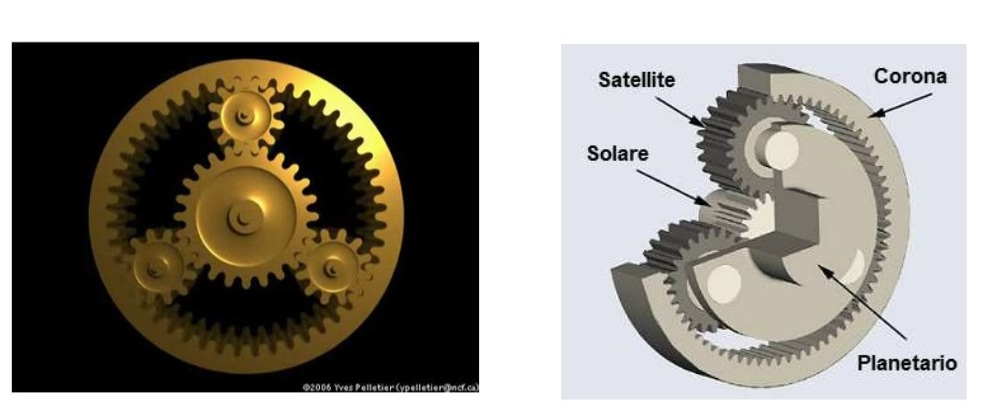
\includegraphics[width=0.6\linewidth]{Epicicloidale.jpeg}
    \caption{Architettura Costruttiva Di Un Riduttore Epicicloidale: Solare Centrale ($s$), Terna Di Satelliti Intermedi ($p$), Portasatelliti O Planetario ($c$) E Corona Circolare Esterna A Dentatura Interna ($r$).}
\end{figure}

\begin{enumerate}
    \item \textbf{Solare (\textit{Sun Gear}, $s$)}: Ruota dentata cilindrica centrale a dentatura esterna montata sull'albero d'ingresso, con $z_s$ denti e velocità angolare $\omega_s$.
    \item \textbf{Satelliti (\textit{Planet Gears}, $p$)}: $n_p \ge 3$ ruote dentate identiche con $z_p$ denti, equispaziate angolarmente a $360^\circ/n_p$, che ingranano simultaneamente con il solare all'interno e con la corona all'esterno.
    \item \textbf{Portasatelliti o Planetario (\textit{Planet Carrier}, $c$)}: Braccio strutturale imperniato sull'albero principale con velocità angolare $\omega_c$, recante i perni su cui ruotano liberamente i satelliti tramite cuscinetti a rullini.
    \item \textbf{Corona (\textit{Ring Gear}, $r$)}: Anello rigido a \textbf{dentatura interna} concentrico al solare, con $z_r$ denti e velocità angolare $\omega_r$, entro cui alloggiano i satelliti.
\end{enumerate}

La congruenza geometrica dei diametri primitivi a parità di modulo $m$ ($d_r = d_s + 2d_p$) impone il vincolo sui numeri di denti:
\[
    z_r = z_s + 2 z_p
\]
\newpage
\subsection{Formalizzazione Analitica: La Formula Di Willis}

La mobilità degli assi dei satelliti impedisce l'applicazione diretta delle relazioni per rotismi ordinari. Si ricorre quindi al \textbf{metodo di inversione cinematica di Willis}, imponendo al sistema la velocità angolare virtuale $-\omega_c$. Nel sistema relativo solidale al portasatelliti ($\omega_c' = \omega_c - \omega_c = 0$), il meccanismo opera come un rotismo ordinario ad assi fissi.

Il \textbf{rapporto fondamentale di Willis} $p_0$ è definito dal rapporto tra le velocità relative della corona e del solare rispetto al portasatelliti:
\[
    p_0 = \frac{\omega_r - \omega_c}{\omega_s - \omega_c}
    \label{eq:willis_fondamentale}
\]
Nel rotismo a portasatelliti fermo, il contatto esterno tra solare e satelliti introduce un'inversione di polarità, mentre l'ingranamento interno tra satelliti e corona conserva il verso; l'accoppiamento globale presenta quindi una singola inversione di segno:
\[
    p_0 = -\frac{z_s}{z_r}
    \label{eq:rapporto_willis_denti}
\]
Uguagliando le equazioni precedenti si ricava la \textbf{Formula di Willis}:
\[
    \omega_r - \omega_c = -\frac{z_s}{z_r} \cdot (\omega_s - \omega_c) \implies z_r \omega_r + z_s \omega_s = (z_r + z_s) \omega_c
    \label{eq:formula_willis_risolta}
\]
Quest'equazione evidenzia che il rotismo possiede \textbf{due gradi di libertà cinematici}. Per funzionare con un singolo ingresso e una singola uscita, uno dei tre membri ($s, c, r$) deve essere bloccato a telaio ($\omega = 0$).

\subsection{Configurazioni Operative Dei Rotismi Epicicloidali}

A seconda del membro vincolato e della scelta degli assi di ingresso e uscita, si definiscono tre regimi operativi:

\begin{figure}[H]
    \centering
    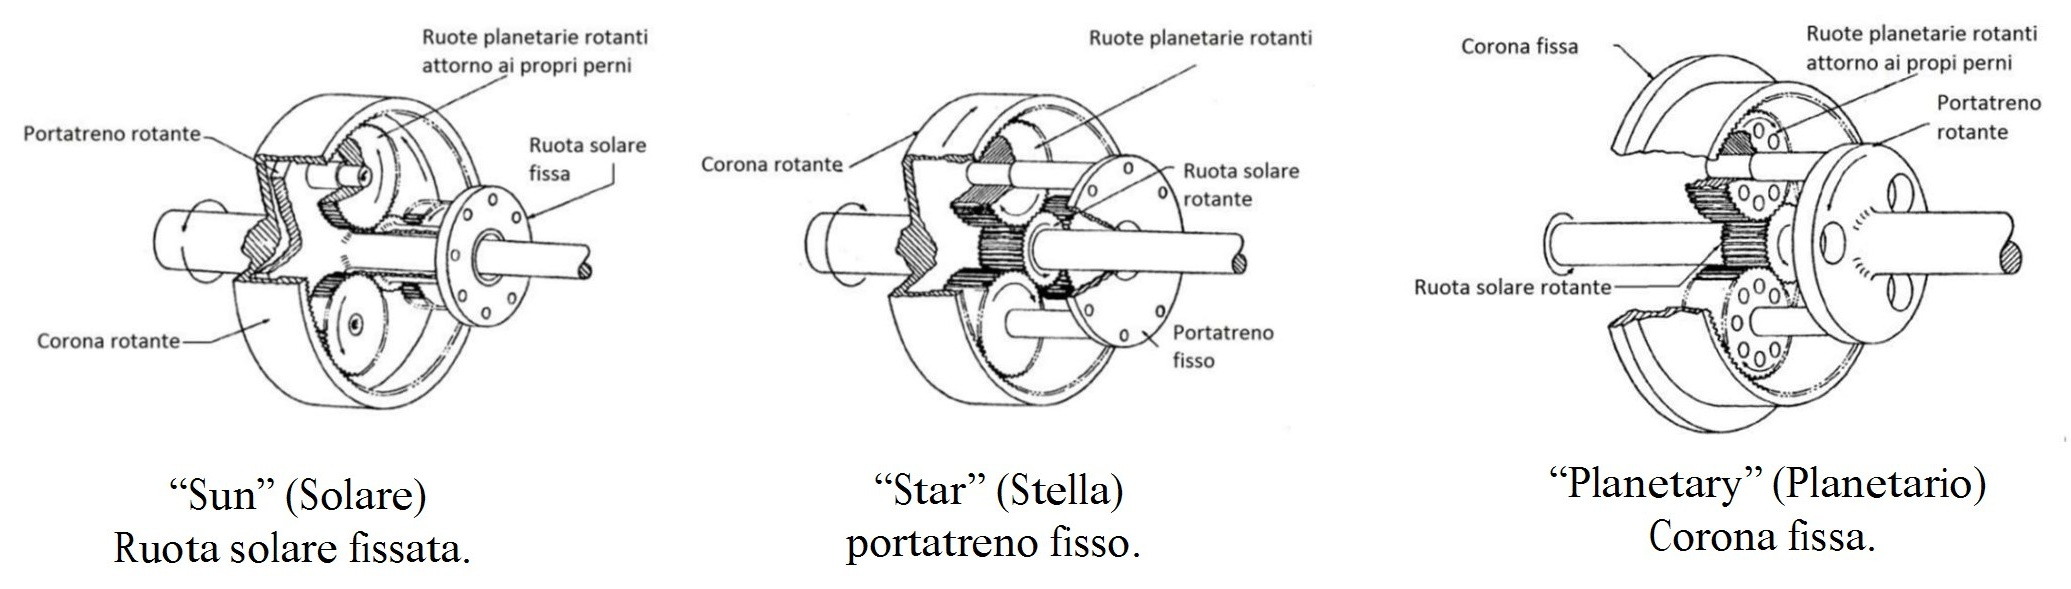
\includegraphics[width=0.65\linewidth]{ConfigEpicicloidale.jpeg}
    \caption{Le Tre Configurazioni Operative Fondamentali: (a) Configurazione Planetaria Con Corona Fissa, (b) Configurazione Solare Con Solare Bloccato, (c) Configurazione A Stella Con Portasatelliti Fisso.}
    \label{fig:config_epicicloidale}
\end{figure}

\begin{description}
    \item[1. Configurazione ``Planetary'' (Corona Fissa):]
    Configurazione primaria nei riduttori per robotica. Corona bloccata a telaio ($\omega_r = 0$), ingresso sul solare ($\omega_{\text{in}} = \omega_s$) e uscita sul portasatelliti collegato al link ($\omega_{\text{out}} = \omega_c$). Ponendo $\omega_r = 0$ in Eq.~\eqref{eq:formula_willis_risolta}:
    \[
        z_s \omega_s = (z_r + z_s) \omega_c \implies \tau = \frac{\omega_{\text{out}}}{\omega_{\text{in}}} = \frac{\omega_c}{\omega_s} = \frac{z_s}{z_s + z_r} = \frac{1}{1 + \frac{z_r}{z_s}}
        \label{eq:tau_planetary}
    \]
    Essendo $z_r > z_s$, si ottiene $\tau > 0$ (rotazione equiversa), con valori tipicamente compresi tra $1/3$ e $1/10$.

    \item[2. Configurazione ``Solar'' (Solare Fisso):]
    Solare vincolato a terra ($\omega_s = 0$), ingresso sulla corona ($\omega_{\text{in}} = \omega_r$) e uscita sul portasatelliti ($\omega_{\text{out}} = \omega_c$). Dall'Eq.~\eqref{eq:formula_willis_risolta}:
    \[
        z_r \omega_r = (z_r + z_s) \omega_c \implies \tau = \frac{\omega_c}{\omega_r} = \frac{z_r}{z_r + z_s} = \frac{1}{1 + \frac{z_s}{z_r}}
    \]
    Il rapporto di riduzione risultante è contenuto ($\tau \approx 0.7 \div 0.9$); trova impiego come moltiplicatore di velocità o ripartitore di coppia.

    \item[3. Configurazione ``Star'' o a Stella (Portasatelliti Fisso):]
    Portasatelliti bloccato a telaio ($\omega_c = 0$). I perni non orbitano e il sistema si comporta come un rotismo ordinario ad assi fissi, con i satelliti operanti da ruote oziose. L'ingresso è sul solare ($\omega_{\text{in}} = \omega_s$) e l'uscita sulla corona ($\omega_{\text{out}} = \omega_r$). Ponendo $\omega_c = 0$ in Eq.~\eqref{eq:formula_willis_risolta}:
    \[
        z_r \omega_r + z_s \omega_s = 0 \implies \tau = \frac{\omega_r}{\omega_s} = -\frac{z_s}{z_r}
    \]
    Il senso di rotazione risulta invertito ($\tau < 0$), con rapporti compresi tra $-1/2$ e $-1/6$.
\end{description}

\subsection{Riduttori Speciali Ad Alta Precisione: L'Harmonic Drive}

I riduttori a onda di deformazione elastica (\textbf{Harmonic Drive} o \textit{strain wave gears}), brevettati da C. Walton Musser nel 1955, costituiscono la soluzione dominante per l'azionamento dei giunti rotoidali in robot antropomorfi, cobot e sistemi avionici o aerospaziali.

\subsubsection{Costituzione Meccanica Ed Elementi Costitutivi}

Il meccanismo è articolato su tre componenti coassiali (Figura~\ref{fig:harmonic_drive_detail}):

\begin{figure}[H]
    \centering
    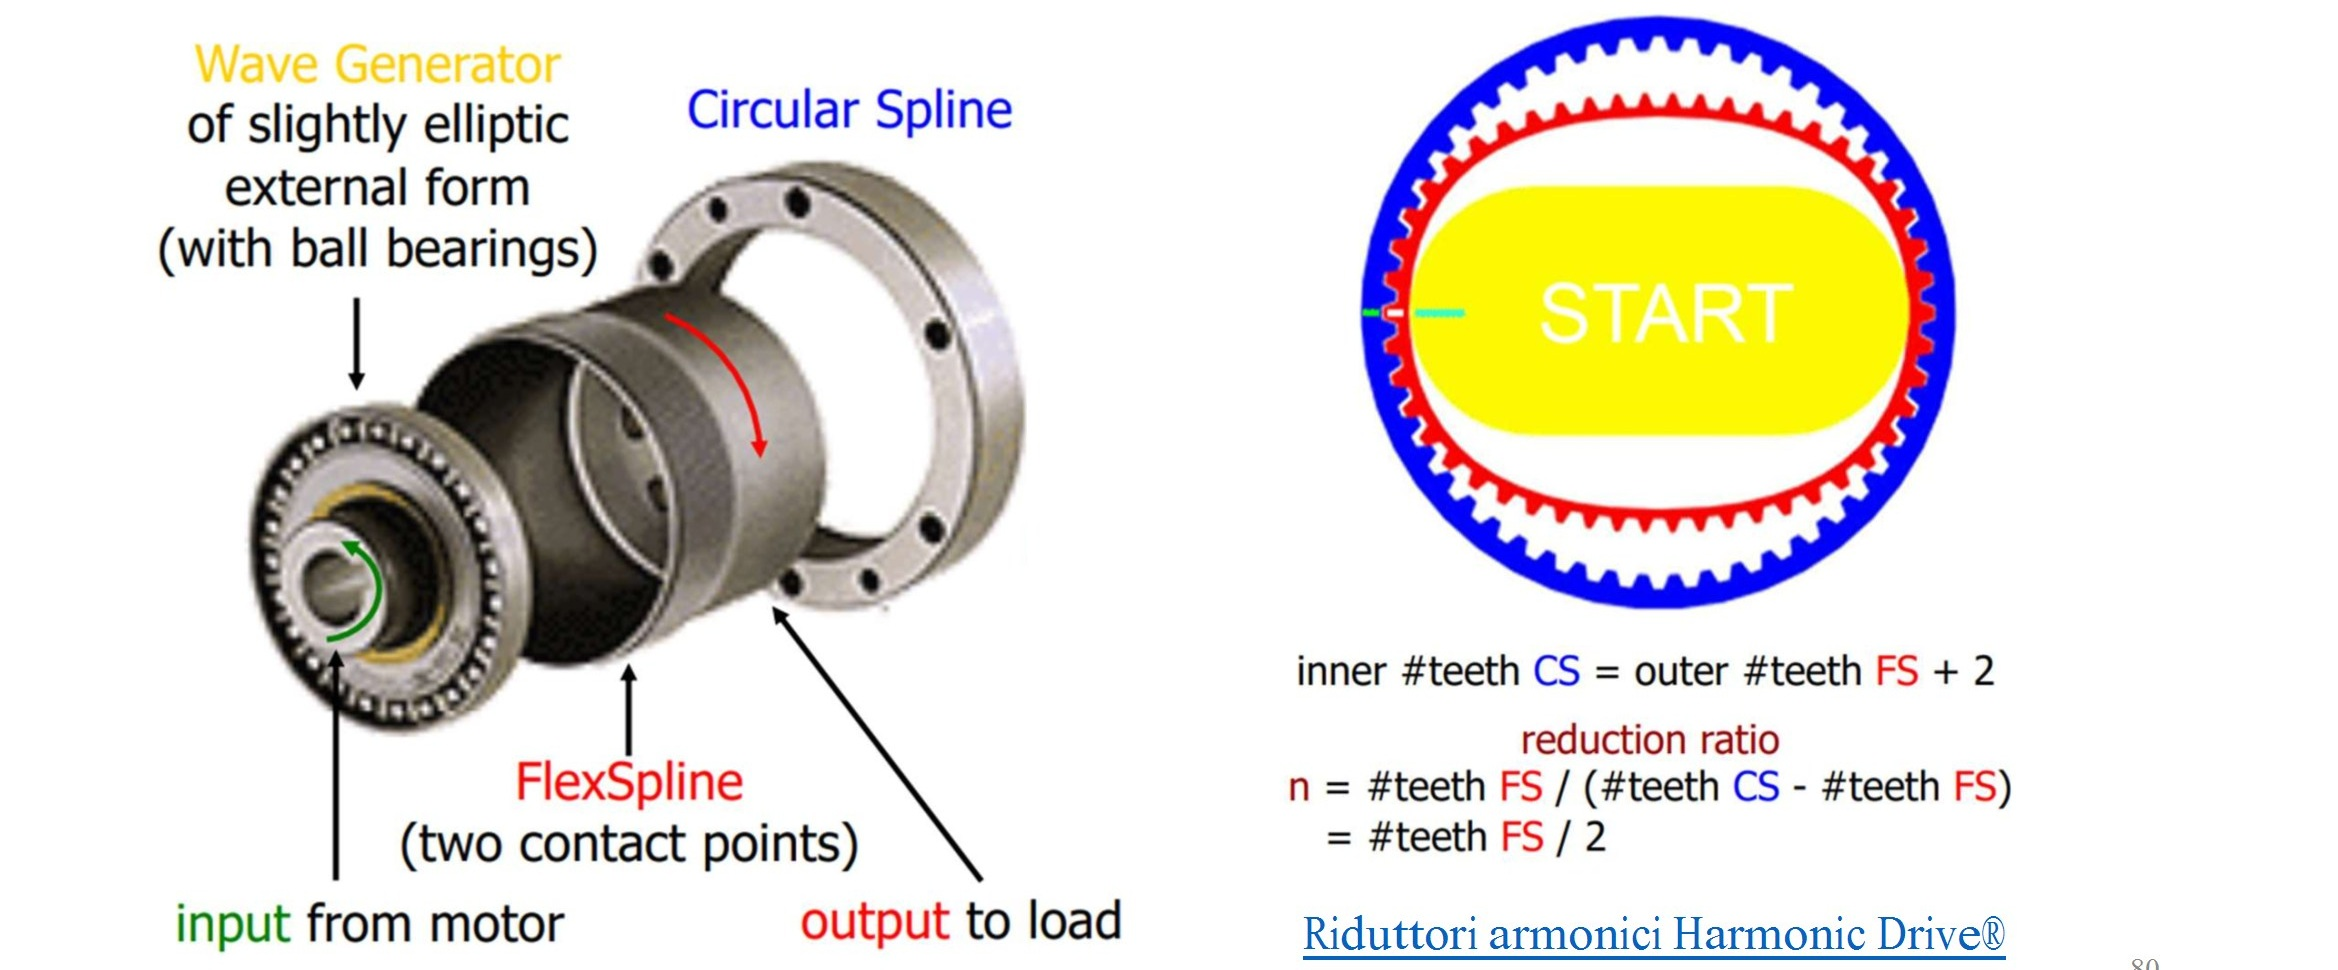
\includegraphics[width=0.75\linewidth]{HarmonicDrive.jpeg}
    \caption{Componenti Dell'Harmonic Drive: (1) Wave Generator Ellittico, (2) FlexSpline Deformabile A Tazza Con Dentatura Esterna, (3) Circular Spline Rigida A Dentatura Interna.}
    \label{fig:harmonic_drive_detail}
\end{figure}

\begin{enumerate}
    \item \textbf{Wave Generator (Generatore d'Onda, WG)}: Elemento d'ingresso calettato sull'albero motore, composto da una camma a profilo \textbf{ellittico} inserita forzatamente in un cuscinetto a sfere deformabile a parete sottile; la sua rotazione genera un'onda radiale viaggiante.
    \item \textbf{FlexSpline (Boccola Deformabile Flessibile, FS)}: Tazza cilindrica a parete sottile in acciaio legato ad alto limite di fatica. L'estremità aperta presenta una \textbf{dentatura esterna}, mentre la base chiusa è collegata all'albero d'uscita del giunto. L'alloggiamento del Wave Generator impone all'estremità aperta la sagoma ellittica della camma.
    \item \textbf{Circular Spline (Corona Circolare Rigida, CS)}: Anello rigido solidale alla struttura, provvisto di \textbf{dentatura interna} con modulo e passo identici a quelli del FlexSpline.
\end{enumerate}

\newpage

\subsubsection{Principio Cinematico Di Funzionamento E Derivazione Del Rapporto Di Riduzione}

Il principio cinematico si fonda sulla differenza del numero di denti tra i due elementi ingrananti:
\[
    z_{\text{CS}} - z_{\text{FS}} = 2
    \label{eq:differenza_denti_hd}
\]
La Circular Spline possiede due denti in più rispetto al FlexSpline.

Con il Wave Generator posizionato all'interno del FlexSpline:
\begin{itemize}
    \item In corrispondenza dell'\textbf{asse maggiore dell'ellisse}, l'eccentricità porta i denti del FlexSpline a ingranare nei vani della Circular Spline per circa il $30\%$ della dentatura complessiva;
    \item In corrispondenza dell'\textbf{asse minore dell'ellisse}, la contrazione radiale disimpegna totalmente le dentature, escludendo il contatto.
\end{itemize}

La rotazione oraria del Wave Generator propaga le due zone di presa. A seguito di una rotazione completa di $360^\circ$ del Wave Generator, il vincolo con la Circular Spline fissa ($z_{\text{FS}} = z_{\text{CS}} - 2$) impone al FlexSpline un arretramento relativo di 2 passi polari.

Con Circular Spline fissa, ingresso su Wave Generator e uscita su FlexSpline, il rapporto di trasmissione risulta:
\[
    \tau_{\text{HD}} = \frac{\omega_{\text{out}}}{\omega_{\text{in}}} = \frac{\omega_{\text{FS}}}{\omega_{\text{WG}}} = -\frac{z_{\text{CS}} - z_{\text{FS}}}{z_{\text{FS}}} = -\frac{2}{z_{\text{FS}}}
    \label{eq:formula_hd}
\]
Il segno negativo indica che il FlexSpline d'uscita ruota in verso opposto a quello del motore.

\paragraph{Esempio Numerico di Calcolo}
Per un'unità con $z_{\text{FS}} = 200$ denti e $z_{\text{CS}} = 202$ denti, l'Eq.~\eqref{eq:formula_hd} fornisce:
\[
    \tau_{\text{HD}} = -\frac{2}{200} = -\frac{1}{100} = -0.01
\]
Il gruppo realizza un rapporto di riduzione di $100:1$ in un solo stadio, moltiplicando la coppia dell'albero motore di un fattore $100$ al netto delle perdite di rendimento.

\subsubsection{Pregi E Limiti Progettuali}

Le proprietà funzionali caratteristiche comprendono:
\begin{itemize}
    \item \textbf{Assenza Strutturale di Gioco Angolare (\textit{Zero Backlash})}: Il precarico radiale lungo l'asse maggiore assicura l'ingranamento simultaneo su entrambi i fianchi dei denti, eliminando il gioco d'inversione e garantendo ripetibilità nell'ordine dell'arco di secondo ($\text{arcsec}$).
    \item \textbf{Ingombri Assiali e Radiali Minimi}: La conformazione a tazza cava consente il passaggio coassiale di linee di segnale e potenza (\textit{hollow shaft design}).
    \item \textbf{Compromesso: Cedevolezza Torsionale}: La flessibilità del FlexSpline introduce un comportamento da molla torsionale non lineare di rigidezza $k_{\text{tor}}$, con risonanze a bassa frequenza ($10 \div 30\,\si{\hertz}$) durante interazioni dinamiche rapide. Il loro smorzamento richiede l'adozione di doppi encoder (a monte e a valle del giunto) nell'anello di controllo.
\end{itemize}

\newpage

% AA Parte 5 - Attuazione Cedevole E Soft Robotics

\section{Attuazione Cedevole E Soft Robotics}

La robotica industriale convenzionale si basa sul principio della \textbf{massima rigidezza strutturale} per assicurare accuratezze centesimali a carichi massimi, impiegando leghe rigide e azionamenti ad elevata impedenza meccanica. Tuttavia, in contesti di interazione fisica diretta con operatori umani (\textit{physical Human-Robot Interaction}, pHRI) o manipolazione di oggetti fragili in ambienti non strutturati, tale rigidezza presenta vincoli critici di sicurezza.

La \textbf{Soft Robotics} supera tali limiti integrando meccanismi deformabili, viscoelastici e a cedevolezza passiva calibrata, sulla base di tre motivazioni:

\begin{enumerate}
    \item \textbf{Sicurezza Intrinseca Passiva (\textit{Intrinsic Safety})}: In caso di avaria sensoriale o di controllo, un attuatore a cedevolezza intrinseca dissipa l'energia dell'urto per deformazione strutturale passiva prima dell'intervento dei sistemi elettronici di arresto, prevenendo lo scarico di forze distruttive.
    \item \textbf{Resilienza e Filtraggio Meccanico dei Sovraccarichi d'Urto}: Nelle collisioni rigide, le decelerazioni generano carichi impulsivi ($F = \Delta p / \Delta t \to \infty$) sui denti dei riduttori. La cedevolezza strutturale opera come filtro passa-basso meccanico, prolungando la durata $\Delta t$ dell'impatto e riducendo il picco di forza trasmesso all'azionamento.
    \item \textbf{Accumulo e Restituzione ciclica di Energia Elastica}: Ispirandosi all'azione muscolo-tendinea biologica, gli attuatori cedevoli immagazzinano energia potenziale $E = \frac{1}{2} k \Delta x^2$ durante le decelerazioni e la rilasciano nelle accelerazioni, riducendo i consumi di picco e permettendo movimenti esplosivi (salti, lanci) con potenze istantanee superiori a quella nominale del motore.
\end{enumerate}

\subsection{Muscoli Pneumatici Artificiali (PAM - Pneumatic Artificial Muscles)}

Tra i trasduttori cedevoli figurano i \textbf{Muscoli Pneumatici Artificiali} (\textit{PAM}), noti principalmente come \textbf{muscoli di McKibben}, ideati da Joseph L. McKibben negli anni '50 come dispositivi protesici.

\begin{figure}[H]
    \centering
    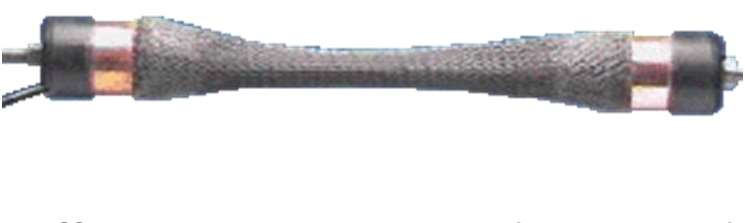
\includegraphics[width=0.4\linewidth]{McKibbenMuscle.jpg}
    \caption{Muscolo Pneumatico Di McKibben}
\end{figure}

\subsubsection{Costruzione E Cinematica Di Contrazione}
Il muscolo di McKibben è costituito da:
\begin{itemize}
    \item Una \textbf{membrana tubolare interna} pneumatica in elastomero siliconico o lattice;
    \item Una \textbf{guaina esterna intrecciata a maglia di losanga} in fili polimerici (nylon, Kevlar) o metallici \textbf{inestensibili}.
\end{itemize}

L'iniezione di aria a pressione relativa $p$ induce la dilatazione radiale della membrana elastomerica. Poiché i fili della guaina sono inestensibili e mutano il loro angolo d'intreccio $\theta_b$, la dilatazione radiale impone la \textbf{contrazione assiale} della struttura; il trasduttore eroga dunque unicamente \textbf{forza di richiamo tensile}.

La forza traente $F$ dipende dalla pressione $p$ e dalla deformazione assiale adimensionale $\epsilon = (l_0 - l)/l_0$, dove $l_0$ è la lunghezza a riposo e $l$ la lunghezza istantanea:
\[
    F(p, \epsilon) = \frac{p \cdot d_0^2 \cdot \pi}{4} \cdot \left[ \frac{3 \cos^2(\theta_b) - 1}{\sin^2(\theta_{b0})} \right]
    \label{eq:forza_mckibben}
\]
dove $\theta_b$ è l'angolo di intreccio istantaneo. All'angolo di equilibrio $\theta_b \approx 54^\circ 44'$, il termine tra parentesi si annulla e la forza tensile decade a zero indipendentemente dal valore di $p$. La massima contrazione assiale utile risulta compresa tra il $20\%$ e il $30\%$ di $l_0$.

\subsubsection{Regimi Operativi Fondamentali}

Il comportamento dell'attuatore si articola in due modalità operative:

\noindent
\begin{minipage}[t]{0.48\textwidth}
    \textbf{Operatività a Carico Costante}
    \par\vspace{0.2cm}
    Applicata una massa gravante $\bm{M}$, per $p=0$ il muscolo si estende alla lunghezza massima $l_{\text{max}}$. All'aumentare della pressione ($p_2 > p_1$), il diametro si dilata e la lunghezza si riduce ($l_2 < l_1 < l_{\text{max}}$), sollevando il carico di un'altezza corrispondente alla variazione assiale.
    \begin{figure}[H]
        \centering
        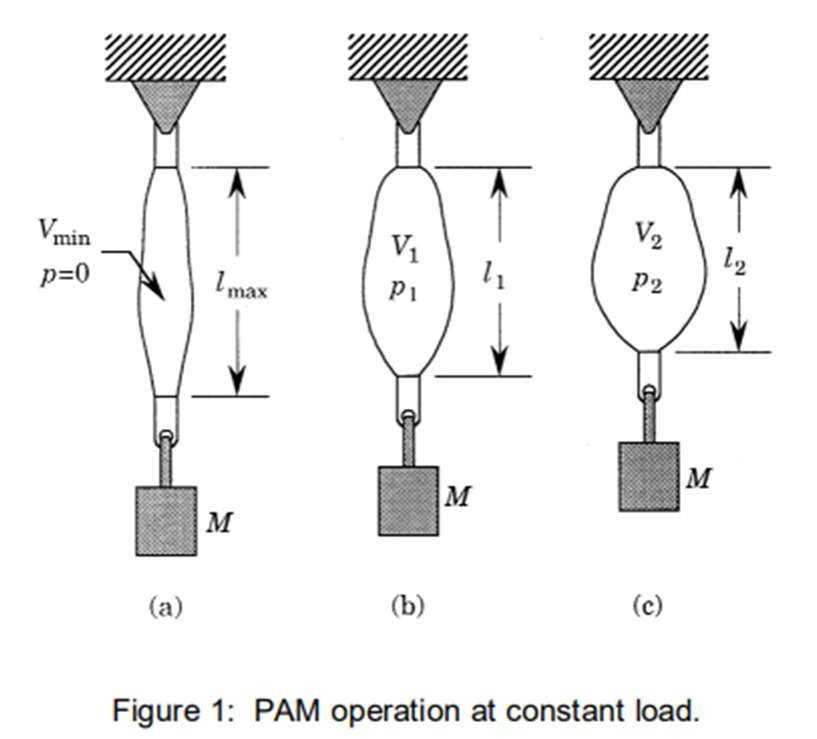
\includegraphics[width=0.75\linewidth]{CaricoCostante.jpg}
        \caption{Risposta a carico costante: contrazione all'aumentare della pressione.}
        \label{fig:carico_costante}
    \end{figure}
\end{minipage}
\hfill
\begin{minipage}[t]{0.48\textwidth}
    \textbf{Operatività a Pressione Costante}
    \par\vspace{0.2cm}
    A pressione $p$ costante, diminuendo il carico applicato da $\bm{M}_1$ a $\bm{M}_2$, la pressione interna incrementa il diametro della calza, inducendo un accorciamento fino al nuovo equilibrio; per $\bm{M}=0$ si ottiene la minima lunghezza $l_{\text{min}}$.
    \begin{figure}[H]
        \centering
        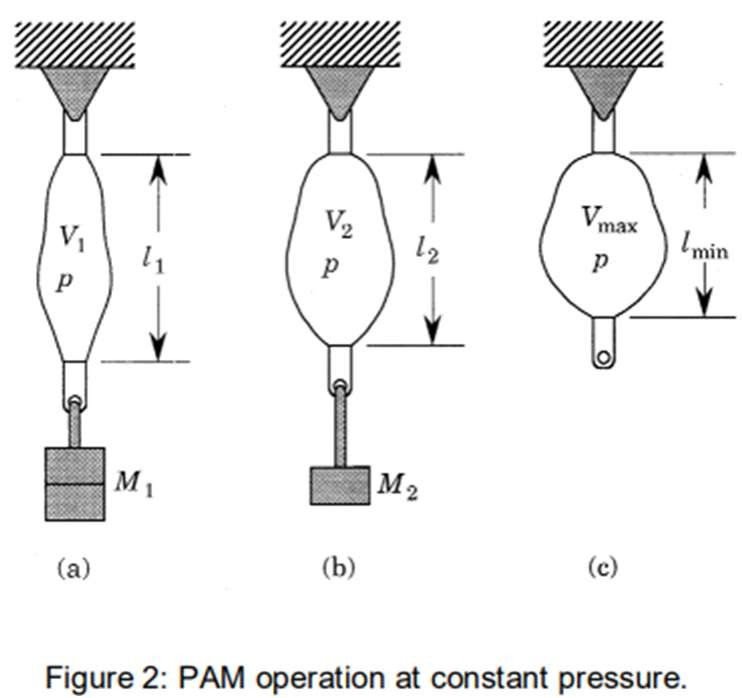
\includegraphics[width=0.75\linewidth]{PressioneCostante.jpg}
        \caption{Risposta a pressione costante: contrazione al diminuire del carico.}
        \label{fig:pressione_costante}
    \end{figure}
\end{minipage}

\subsubsection{Attuazione Antagonistica E Controllo Disaccoppiato Di Rigidità}

Poiché i PAM esercitano \textbf{esclusivamente trazione}, la movimentazione bidirezionale di un giunto rotante richiede una configurazione a \textbf{coppia antagonista}, analoga al funzionamento dei muscoli scheletrici bicipite-tricipite.

\begin{figure}[H]
    \centering
    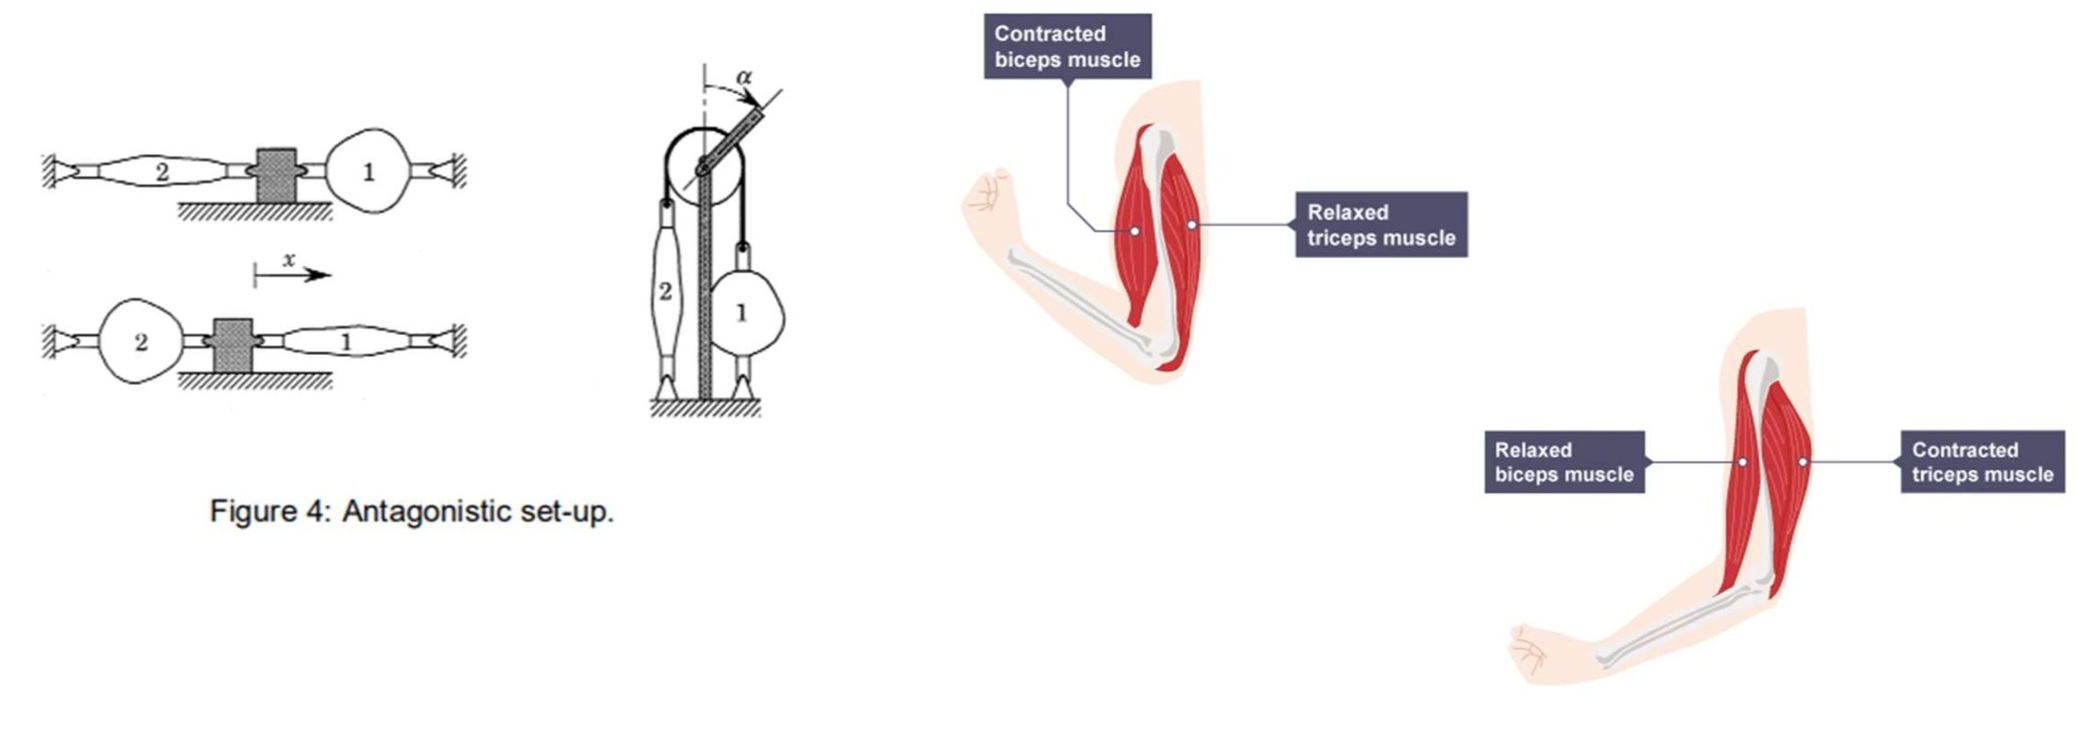
\includegraphics[width=0.7\linewidth]{FunzAntag.jpeg}
    \caption{Configurazione antagonista di due muscoli PAM: regolazione simultanea dell'angolo di equilibrio $\theta_j$ del giunto e della rigidezza torsionale $K_{\text{joint}}$.}
    \label{fig:funz_antag}
\end{figure}

Due muscoli PAM ($M_1$ e $M_2$) sono collegati a una puleggia solidale all'asse del giunto (Figura~\ref{fig:funz_antag}). Le pressioni di alimentazione $p_1$ e $p_2$ determinano due parametri indipendenti:
\begin{itemize}
    \item \textbf{Pressione Differenziale ($\Delta p = p_1 - p_2$)}: Produce un momento torcente netto, determinando l'\textbf{angolo di posizione del giunto} $\theta_j$;
    \item \textbf{Pressione Comune o di Co-attivazione ($p_c = \frac{p_1 + p_2}{2}$)}: Determina il precarico interno. Poiché la rigidezza meccanica della camera d'aria aumenta con la pressione assoluta, incrementare $p_c$ lascia invariata la posizione e \textbf{aumenta la rigidezza torsionale passiva} del giunto ($K_{\text{joint}}$), permettendo di passare da elevata cedevolezza per pHRI ad elevata rigidezza per lavorazioni seriali.
\end{itemize}

\newpage

\subsection{Attuatori Con Elementi Elastici Intenzionali: SEA E VSA}

Nei manipolatori rigidi tradizionali il controllo di forza viene eseguito tramite anelli di impedenza attiva su celle di carico a flangia, con prestazioni limitate negli urti ad alta frequenza da ritardi d'attuazione e larghezza di banda finita. Nel 1995 Gill Pratt e Matthew Williamson proposero quindi l'integrazione di \textbf{elementi elastici calibrati all'interno della catena cinematica}.

\subsubsection{Attuatori Elastici Seriali (SEA - Serial Elastic Actuators)}

Un \textbf{Attuatore Elastico Seriale} (SEA) incorpora un elemento elastico a rigidezza nota $k$ (molla torsionale o molle a tazza) disposto in serie tra riduttore e carico.

\begin{figure}[H]
    \centering
    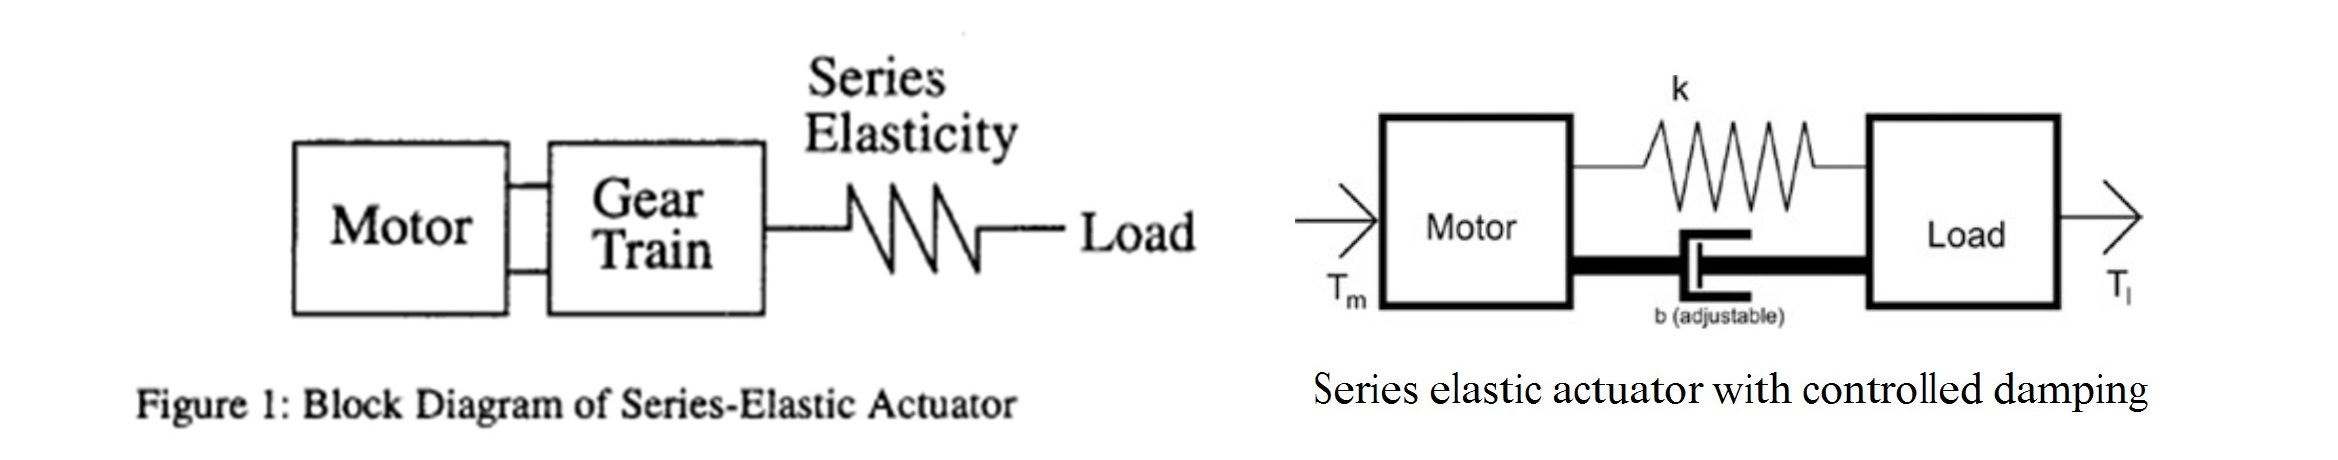
\includegraphics[width=0.85\textwidth]{SEA.jpeg}
    \caption{Schema Concettuale A Blocchi Di Un Attuatore Elastico Seriale (SEA): Motore E Riduttore Azionano La Molla In Serie, La Cui Deflessione Elastica Comanda Il Moto Del Carico.}
    \label{fig:sea_concept}
\end{figure}

L'interposizione della molla introduce tre proprietà funzionali:
\begin{enumerate}
    \item \textbf{Trasformazione del Controllo di Forza in Controllo di Posizione}: La forza (o coppia) $\tau$ trasmessa al carico è correlata alla deformazione elastica dalla legge di Hooke:
    \[
        F = k \cdot (x_{\text{mot}} - x_{\text{load}}) = k \cdot \Delta x
        \label{eq:hooke_sea}
    \]
    La misura della deflessione differenziale $\Delta x$ tra i capi della molla tramite encoder di posizione fornisce una stima della forza priva del rumore ad alta frequenza tipico di sensori piezoelettrici o estensimetrici.
    \item \textbf{Tolleranza Strutturale ai Sovraccarichi d'Urto}: La molla isola meccanicamente i denti del riduttore dai carichi impulsivi esterni.
    \item \textbf{Compromesso sulla Banda Passante}: La presenza dell'elasticità introduce poli complessi coniugati nella funzione di trasferimento, limitando la banda passante in posizione alla frequenza naturale $\omega_n = \sqrt{k/J_L}$.
\end{enumerate}

\paragraph{Architettura Elettromeccanica di un SEA Commerciale}
La figura riporta l'architettura costruttiva di un attuatore lineare SEA basato sullo schema originale di Pratt e Williamson.

\noindent
\begin{minipage}[t]{0.48\textwidth}
    La catena cinematica comprende:
    \begin{enumerate}
        \item Servomotore in corrente continua con riduttore planetario (\textbf{DC motor with gearbox});
        \item Vite a ricircolo di sfere (\textbf{ball screw}) e chiocciola flangiata (\textbf{ball nut plate}) per la conversione rotazione-traslazione;
        \item Carrello mobile (\textbf{moving sub-assembly}) scorrevole lungo aste rettificate di guida (\textbf{guide rods});
        \item Due molle elicoidali in acciaio precaricate e contrapposte (\textbf{springs}), interposte tra chiocciola e asta d'uscita;
        \item Asta di spinta d'uscita (\textbf{moving rod}) provvista di terminale per la connessione al carico (\textbf{load connection terminal}).
    \end{enumerate}
\end{minipage}
\hfill
\begin{minipage}[t]{0.48\textwidth}
    \begin{figure}[H]
        \centering
        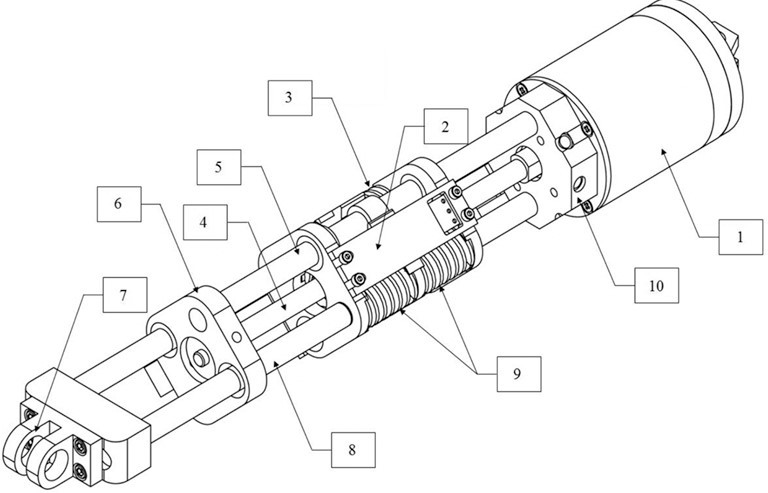
\includegraphics[width=0.99\linewidth]{SEAStruct.jpg}
        \caption{Spaccato Costruttivo Di Un Attuatore Lineare SEA A Vite Con Molle Di Richiamo Contrapposte.}
    \end{figure}
\end{minipage}

\newpage

\subsubsection{Attuatori A Rigidità Variabile (VSA - Variable Stiffness Actuators)}

A differenza dei SEA, in cui la rigidezza $k$ è costante, gli \textbf{Attuatori a Rigidità Variabile} (\textit{VSA}) consentono di regolare la rigidezza passiva $k_{\text{var}}$ indipendentemente dalla posizione del giunto.

\begin{figure}[H]
    \centering
    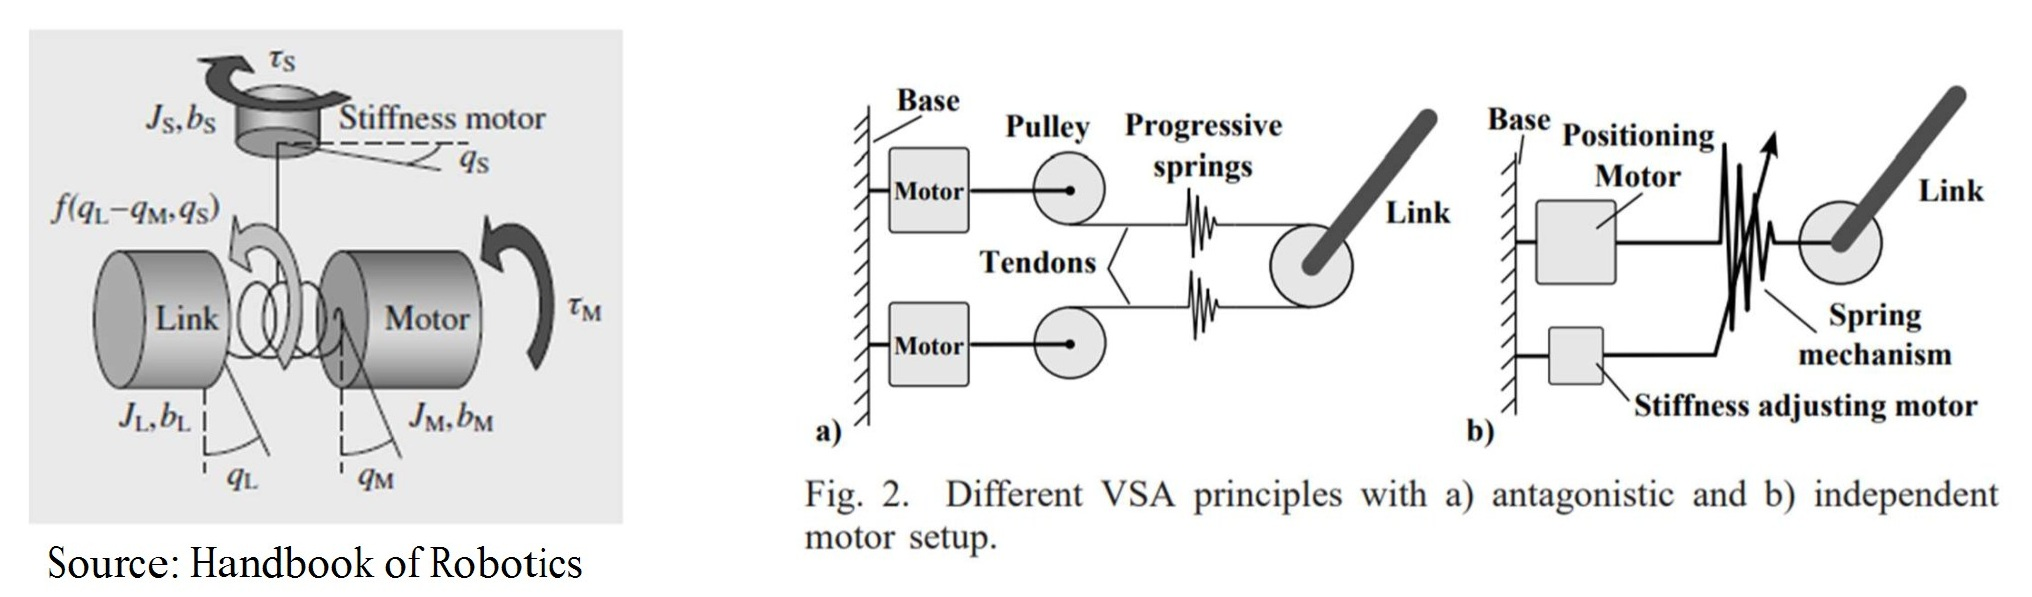
\includegraphics[width=0.85\textwidth]{VSA.jpeg}
    \caption{Schema Concettuale Di Un Attuatore A Rigidità Variabile (VSA): Un Loop Indipendente Regola L'Angolo Di Equilibrio $\Theta$, Mentre Un Secondo Sottosistema Modula La Rigidità Passiva $\Sigma$.}
    \label{fig:vsa_concept}
\end{figure}
Un attuatore VSA dispone di \textbf{due gradi di libertà cinematici interni} gestiti da attuatori indipendenti:
\begin{enumerate}
    \item Il primo attuatore comanda la \textbf{posizione angolare di equilibrio} $\theta_d$;
    \item Il secondo modula la \textbf{rigidità passiva} $\sigma = \frac{\partial \tau}{\partial \theta}$.
\end{enumerate}
La variazione di rigidezza è realizzata prevalentemente mediante due schemi costruttivi:
\begin{itemize}
    \item \textbf{Architettura Antagonista Non Lineare}: Due motori azionano il medesimo giunto tramite molle a rigidezza progressiva non lineare (es. $F \propto x^3$). La rotazione concorde comanda la posa del giunto, mentre la rotazione discorde precarica le molle aumentandone la rigidezza tangenziale locale senza alterare l'angolo dell'articolazione.
    \item \textbf{Architettura a Modulazione Meccanica Parametrica}: Un motore primario (\textit{positioning motor}) aziona la catena cinematica, mentre un motore ausiliario di regolazione (\textit{stiffness motor}) interviene sulla geometria dell'elemento elastico, traslando il fulcro di una leva, variando il precarico di una molla a spirale o alterando la lunghezza libera di una lamina flessibile.
\end{itemize}

\subsection{Panoramica Tassonomica Su Altre Tecnologie Di Attuazione Morbida}

Oltre alle soluzioni a fluido (PAM) e con molle meccaniche (SEA/VSA), la Soft Robotics e la microrobotica impiegano trasduttori basati su \textbf{materiali attivi} (\textit{smart materials}):

\begin{itemize}
    \item \textbf{Attuatori Elettrostatici ed Elettromagnetici}: Basati su forze coulombiane o di Lorentz su microscala; impiegati in dispositivi MEMS (\textit{Micro-Electro-Mechanical Systems}) con tempi di risposta sub-millisecondo e corse microscopiche.
    \item \textbf{Attuatori Piezoelettrici}: Cristalli ceramici (es. Titanato Zirconato di Piombo, PZT) a deformazione proporzionale al campo elettrico applicato; sviluppano forze elevate ad alta frequenza ($\si{\kilo\hertz}$), indicati per microposizionamento e smorzamento attivo di vibrazioni.
    \item \textbf{Materiali Elettrostrittivi e Magnetostrittivi}: Leghe (es. Terfenol-D) con deformazione proporzionale al quadrato del campo magnetico o di polarizzazione dielettrica.
    \item \textbf{Leghe a Memoria di Forma (SMA - Shape Memory Alloys)}: Leghe metalliche binarie (tipicamente Nitinol, Nichel-Titanio) a transizione di fase termomeccanica martensitica reversibile. Il riscaldamento per effetto Joule induce il passaggio dalla fase martensitica a bassa temperatura a quella austenitica ad alta temperatura, ripristinando la geometria originaria con forze specifiche elevate. Presentano rendimento energetico contenuto ($< 2\%$) e tempi di raffreddamento prolungati.
    \newpage
    \item \textbf{Polimeri Elettroattivi (EAP - Electroactive Polymers)}: Membrane elastomeriche dielettriche interposte tra elettrodi deformabili. L'applicazione di tensioni elevate ($> \SI{1}{\kilo\volt}$) produce una pressione elettrostatica (pressione di Maxwell) che assottiglia il dielettrico inducendone la dilatazione superficiale, con deformazioni utili del $30 \div 50\%$.
    \item \textbf{Attuatori a Nanotubi di Carbonio (CNT)}: Basati sull'iniezione elettrochimica di cariche in fogli di grafene, garantiscono elevata resistenza a trazione e compatibilità con ambienti biologici.
    \item \textbf{Smorzatori Magnetoreologici (MR) e a Dissipazione Controllata}: Dispositivi contenenti microparticelle ferrose sospese in oli minerali. Sotto l'azione di un campo magnetico variabile generato da un solenoide, l'allineamento a dipolo delle particelle muta la viscosità da fluida a semisolida, modulando il coefficiente di smorzamento meccanico per la dissipazione degli impatti.
\end{itemize}

\end{document}
